%%%%%%%%%%%%%%%%%%%%%%%%%%%%%%%%%%%%%%%%%%%%%%%%%%%%
% Document type, global settings, and packages
%%%%%%%%%%%%%%%%%%%%%%%%%%%%%%%%%%%%%%%%%%%%%%%%%%%%

\documentclass[12pt]{report}   %12 point font for Times New Roman
\usepackage{graphicx}  %for images and plots
\usepackage[letterpaper, left=1.5in, right=1in, top=1in, bottom=1in]{geometry}
\usepackage[doublespacing]{setspace}  %use this package to set linespacing as desired
\usepackage{times}  %set Times New Roman as the font
\usepackage[explicit]{titlesec}  %title control and formatting
\usepackage[titles]{tocloft}  %table of contents control and formatting
%\usepackage[backend=bibtex, sorting=none]{biblatex}  %reference manager
\usepackage[bookmarks=true, hidelinks]{hyperref}
\usepackage[page]{appendix}  %for appendices
\usepackage{rotating}  %for rotated, landscape images

\usepackage[round]{natbib}


\usepackage{enumitem}
%\usepackage{listings}
%\usepackage{comment}
\usepackage{color,soul}
%\usepackage{placeins}
\usepackage{float}
\usepackage{multirow}
\usepackage{graphicx}
%\soulregister\cite7
%\soulregister\ref7
%\soulregister\pageref7
%\usepackage{arydshln}
\usepackage{amsmath}

\usepackage{algorithm}
\usepackage[noend]{algpseudocode}

\usepackage[english]{babel}
\usepackage[T1]{fontenc}
\usepackage[utf8]{inputenc}
\usepackage{relsize}
%%%%%%%%%%%%%%%%%%%%%%%%%%%%%
\usepackage{minitoc}
\usepackage{times} 
\usepackage[T1]{fontenc}         
\usepackage{pslatex}

\usepackage{times}
\usepackage{url}
\usepackage{latexsym}
%\usepackage{multibib}
%\usepackage{biblatex}

%included by me
\usepackage{enumitem}
\usepackage{comment}
\usepackage{color,soul}
\usepackage{placeins}
\usepackage{float}
\usepackage{multirow}
\usepackage{graphicx}
\soulregister\cite7
\soulregister\ref7
\soulregister\pageref7
\usepackage{amsmath}
\usepackage{titlesec}
\usepackage[english]{babel}
\usepackage{titlesec}
\usepackage{hyperref}
\usepackage{amssymb}

\usepackage{lastpage}
\usepackage{xcolor}


\setcounter{secnumdepth}{4}
\setcounter{tocdepth}{4}



% \usepackage[latin1]{inputenc}
% \usepackage[T1]{fontenc}
% \usepackage{lmodern}
% \usepackage[rgb]{xcolor}
% \usepackage[author={Atreyee}]{pdfcomment}

\newcommand{\etal}{\textit{et al}.}

\newcommand{\hlcyan}[1]{{\sethlcolor{cyan}\hl{#1}}}
\newcommand{\ignore}[1]{}
\newcommand{\atrcomments}[1]{\textcolor{red}{\textbf{\textit{\underline{#1}}}}}
%\newcommand{\blue}[1]{\textcolor{blue}{#1}}
\newcommand{\blue}[1]{{\leavevmode\color{blue}{#1}}}
\newcommand\myquestions[1]{\textcolor{yellow}{#1}}

%%%%%%%%%%%%%%%%%%%%%%%%%
%\usepackage{enumerate}
%\usepackage{url}
%\usepackage{latexsym}


%algo packages

\usepackage{algorithm}
\usepackage[noend]{algpseudocode}
\usepackage{todonotes}

%%%%%%%%%%%%%%%%%%%%%%%%%%%%%%%%%%%
% Bibliography
%%%%%%%%%%%%%%%%%%%%%%%%%%%%%%%%%%%



%Add your bibliography file here




%\bibliography{references}
% % prevent certain fields in references from printing in bibliography
% \AtEveryBibitem{\clearfield{issn}}
% \AtEveryBibitem{\clearlist{issn}}

% \AtEveryBibitem{\clearfield{language}}
% \AtEveryBibitem{\clearlist{language}}

% \AtEveryBibitem{\clearfield{doi}}
% \AtEveryBibitem{\clearlist{doi}}

% \AtEveryBibitem{\clearfield{url}}
% \AtEveryBibitem{\clearlist{url}}

% \AtEveryBibitem{%
%   \ifentrytype{online}
%     {}
%     {\clearfield{urlyear}\clearfield{urlmonth}\clearfield{urlday}}}

%%%%%%%%%%%%%%%%%%%%%%
% Start of Document
%%%%%%%%%%%%%%%%%%%%%%

\begin{document}
%\doublespacing  %set line spacing

%%%%%%%%%%%%%%%%%%%%%%%%%%%%%%%%%%%%%
% Title Page
%%%%%%%%%%%%%%%%%%%%%%%%%%%%%%%%%%%%%
\currentpdfbookmark{Title Page}{titlePage}  %add PDF bookmark for this page
%% Define your thesis title, your name, your school, and your month and year of graduation here

\newcommand{\thesisTitle}{Towards Effective Domain Adaptation of Dependency Parsing}
\newcommand{\yourName}{Atreyee Mukherjee}
\newcommand{\yourDepartment}{School of Informatics, Computing and Engineering}
\newcommand{\yourSchool}{Indiana University}
\newcommand{\yourMonth}{}
\newcommand{\yourYear}{}

%%%%%%%%%%%%%%%%%%%%%%%%%%%%%%%%%%%%%%%%%%%%%%%%%%%%%%%%%
% Do not edit these lines unless you wish to customize
% the template
%%%%%%%%%%%%%%%%%%%%%%%%%%%%%%%%%%%%%%%%%%%%%%%%%%%%%%%%%



\begin{titlepage}
\newgeometry{top=2in}
\begin{center}

{\large \MakeUppercase{\thesisTitle}}\\
\vspace{7\baselineskip}
\yourName\\
\vfill
Submitted to the faculty of the University Graduate School\\
in partial fulfillment of the requirements\\
for the degree\\
Doctor of Philosophy\\
in the Department of \yourDepartment,\\
\yourSchool\\
\yourMonth{} \yourYear{}

\end{center}
\restoregeometry
\end{titlepage}


%%%%%%%%%%%%%%%%%%%%%%%%%%%%%%%%%%%%%
% Approval Page
%%%%%%%%%%%%%%%%%%%%%%%%%%%%%%%%%%%%%
\pagenumbering{roman}
\setcounter{page}{2} % set the page number appropriately based on the number of intro pages
\newpage
%% Define your committee members. If you have less than 6, simple delete/comment the unused lines

\newcommand{\committeeChairpersonTypedName}{Sandra K{\"u}bler}
\newcommand{\committeeChairpersonPostNominalInitials}{PhD}

\newcommand{\committeeMemberTwoTypedName}{David Crandall}
\newcommand{\committeeMemberTwoPostNominalInitials}{PhD}

\newcommand{\committeeMemberThreeTypedName}{David Leake}
\newcommand{\committeeMemberThreePostNominalInitials}{PhD}

\newcommand{\committeeMemberFourTypedName}{Donald Williamson}
\newcommand{\committeeMemberFourPostNominalInitials}{PhD}

% Uncomment to add another committee member
%\newcommand{\committeeMemberFiveTypedName}{Name}
%\newcommand{\committeeMemberFivePostNominalInitials}{Post-Nominal Initials}

\newcommand{\myRule}{\rule{0.5\textwidth}{0.4pt}}

\newcommand{\approvalDay}{04}
\newcommand{\approvalMonth}{07}
\newcommand{\approvalYear}{2019}

%%%%%%%%%%%%%%%%%%%%%%%%%%%%%%%%%%%%%%%%%%%%%%%%%%%%%%%%%
% Do not edit these lines unless you wish to customize
% the template
%%%%%%%%%%%%%%%%%%%%%%%%%%%%%%%%%%%%%%%%%%%%%%%%%%%%%%%%%


\newgeometry{left=1in}

\begin{center}
 
Accepted by the Graduate Faculty, Indiana University, in partial fulfillment of the requirements for the degree of Doctor of Philosophy.

\end{center}

\vspace{2\baselineskip}

\ifdefined\committeeMemberFourTypedName
Doctoral Committee\\

\null\hfill \myRule\\
\null\hfill \committeeChairpersonTypedName, \committeeChairpersonPostNominalInitials\\
\null\hfill \myRule\\
\null\hfill \committeeMemberTwoTypedName, \committeeMemberTwoPostNominalInitials\\
\null\hfill \myRule\\
\null\hfill \committeeMemberThreeTypedName, \committeeMemberThreePostNominalInitials\\
\null\hfill \myRule\\
\null\hfill \committeeMemberFourTypedName, \committeeMemberFourPostNominalInitials\\

\ifdefined\committeeMemberFiveTypedName
\null\hfill \myRule\\
\null\hfill \committeeMemberFiveTypedName, \committeeMemberFivePostNominalInitials\\
\fi

\fi
\vfill
Date of Defense: \approvalMonth/\approvalDay/\approvalYear
\restoregeometry


%%%%%%%%%%%%%%%%%%%%%%%%%%%%%%%%%%%%%
% Copyright
%%%%%%%%%%%%%%%%%%%%%%%%%%%%%%%%%%%%%
\newpage
%%%%%%%%%%%%%%%%%%%%%%%%%%%%%%%%%%%%%%%%%%%%%%%%%%%%%%%%%
% Do not edit these lines unless you wish to customize
% the template
%%%%%%%%%%%%%%%%%%%%%%%%%%%%%%%%%%%%%%%%%%%%%%%%%%%%%%%%%

\clearpage
\begin{center}

\vspace*{\fill}
Copyright \copyright{} \yourYear{}\\
\yourName
\vspace*{\fill}

\end{center}
\clearpage


%%%%%%%%%%%%%%%%%%%%%%%%%%%%%%%%%%%%%
% Dedication
%%%%%%%%%%%%%%%%%%%%%%%%%%%%%%%%%%%%%
\newpage
% Define your dedication statement here

\newcommand{\yourDedication}{A great dedication goes here.}

%%%%%%%%%%%%%%%%%%%%%%%%%%%%%%%%%%%%%%%%%%%%%%%%%%%%%%%%%
% Do not edit these lines unless you wish to customize
% the template
%%%%%%%%%%%%%%%%%%%%%%%%%%%%%%%%%%%%%%%%%%%%%%%%%%%%%%%%%

\begin{center}

\vspace*{\fill}
\yourDedication\\
\vspace*{\fill}

\end{center}

%%%%%%%%%%%%%%%%%%%%%%%%%%%%%%%%%%%%%
% Acknowledgments
%%%%%%%%%%%%%%%%%%%%%%%%%%%%%%%%%%%%%
\newpage
\phantomsection
\addcontentsline{toc}{chapter}{Acknowledgements}
\begin{centering}
\textbf{ACKNOWLEDGEMENTS}\\
\vspace{\baselineskip}
\end{centering}

%Insert your dedication text here



%%%%%%%%%%%%%%%%%%%%%%%%%%%%%%%%%%%%%
% Abstract
%%%%%%%%%%%%%%%%%%%%%%%%%%%%%%%%%%%%%
\newpage
\phantomsection
\addcontentsline{toc}{chapter}{Abstract}
%%%%%%%%%%%%%%%%%%%%%%%%%%%%%%%%%%%%%%%%%%%%%%%%%%%%%%%%%
% Do not edit these lines unless you wish to customize
% the template
%%%%%%%%%%%%%%%%%%%%%%%%%%%%%%%%%%%%%%%%%%%%%%%%%%%%%%%%%
\newgeometry{left=1in}

\begin{center}

\yourName\\
\MakeUppercase{\thesisTitle}

\end{center}

\vspace{1.5\baselineskip}

%Insert your abstract here
abstract?


\ifdefined\committeeMemberFourTypedName

\null\hfill \myRule\\
\null\hfill \committeeChairpersonTypedName, \committeeChairpersonPostNominalInitials\\
\null\hfill \myRule\\
\null\hfill \committeeMemberTwoTypedName, \committeeMemberTwoPostNominalInitials\\
\null\hfill \myRule\\
\null\hfill \committeeMemberThreeTypedName, \committeeMemberThreePostNominalInitials\\
\null\hfill \myRule\\
\null\hfill \committeeMemberFourTypedName, \committeeMemberFourPostNominalInitials\\

\ifdefined\committeeMemberFiveTypedName
\null\hfill \myRule\\
\null\hfill \committeeMemberFiveTypedName, \committeeMemberFivePostNominalInitials\\
\fi

\fi
\restoregeometry




%%%%%%%%%%%%%%%%%%%%%%%%%%%%%%%%%%%%%
% Table of Contents
%%%%%%%%%%%%%%%%%%%%%%%%%%%%%%%%%%%%%

% Format for Table of Contents
\renewcommand{\cftchapdotsep}{\cftdotsep}  %add dot separators
\renewcommand{\cftchapfont}{\bfseries}  %set title font weight
\renewcommand{\cftchappagefont}{}  %set page number font weight
\renewcommand{\cftchappresnum}{Chapter }
\renewcommand{\cftchapaftersnum}{:}
\renewcommand{\cftchapnumwidth}{5em}
\renewcommand{\cftchapafterpnum}{\vskip\baselineskip} %set correct spacing for entries in single space environment
\renewcommand{\cftsecafterpnum}{\vskip\baselineskip}  %set correct spacing for entries in single space environment
\renewcommand{\cftsubsecafterpnum}{\vskip\baselineskip} %set correct spacing for entries in single space environment
\renewcommand{\cftsubsubsecafterpnum}{\vskip\baselineskip} %set correct spacing for entries in single space environment

%format title font size and position (this also applys to list of figures and list of tables)
\titleformat{\chapter}[display]
{\normalfont\bfseries\filcenter}{\chaptertitlename\ \thechapter}{0pt}{\MakeUppercase{#1}}

\renewcommand\contentsname{Table of Contents}
\currentpdfbookmark{Table of Contents}{TOC}
\begin{singlespace}
\tableofcontents
\end{singlespace}


\clearpage

%%%%%%%%%%%%%%%%%%%%%%%%%%%%%%%%%%%%%
% List of figures and tables
%%%%%%%%%%%%%%%%%%%%%%%%%%%%%%%%%%%%%
\phantomsection
\addcontentsline{toc}{chapter}{List of Tables}
\begin{singlespace}
\setlength\cftbeforetabskip{\baselineskip}  %manually set spacing between entries
\listoftables
\end{singlespace}

\clearpage

\phantomsection
\addcontentsline{toc}{chapter}{List of Figures}
\begin{singlespace}
\setlength\cftbeforefigskip{\baselineskip}  %manually set spacing between entries
\listoffigures
\end{singlespace}

\clearpage

%%%%%%%%%%%%%%%%%%%%%%%%%%%%
%
% Chapters
%
%%%%%%%%%%%%%%%%%%%%%%%%%%%%

%%%%%%%%%%%%%%%%%%%%%%
% formatting
%%%%%%%%%%%%%%%%%%%%%%

% resume page numbering for rest of document
\clearpage
\pagenumbering{arabic}
\setcounter{page}{1} % set the page number appropriately

% Adjust chapter title formatting
\titleformat{\chapter}[display]
{\normalfont\bfseries\filcenter}{\MakeUppercase\chaptertitlename\ \thechapter}{0pt}{\MakeUppercase{#1}}  %spacing between titles
\titlespacing*{\chapter}
  {0pt}{0pt}{30pt}	%controls vertical margins on title
  
% Adjust section title formatting
\titleformat{\section}{\normalfont\bfseries}{\thesection}{1em}{#1}

% Adjust subsection title formatting
\titleformat{\subsection}{\normalfont\bfseries}{\thesubsection}{1em}{#1}

% Adjust subsubsection title formatting
\titleformat{\subsubsection}{\normalfont\itshape}{\thesubsubsection}{1em}{#1}

%%%%%%%%%%%%%%%%
% Chapter 1 - Introduction
%%%%%%%%%%%%%%%%

\chapter{Introduction}

\atrcomments{TBD!!}

Syntactic parsing refers to the process of extracting and analyzing the syntactic structure or representation of a natural language text. This is very useful is a variety of different domains such as machine translation, information retrieval, question answering \cite{hall2008transition}. More formally, we can define it as a structural prediction problem. Hence, there is an input which are sentences; an output, which are syntactic representation of a sentence;  and a model that maps the input to the output. The input sentence is usually split into tokens. The output is represented as trees. Dependency parsing is a type of syntactic parsing analyses the dependency structure of a sentence based on a dependency grammar. As illustrated in figure~\ref{fig:depParsetree}, the words in a sentence are linked with relations (shown using labeled arrows), also known as dependency relation (dependencies) where one word is the dependent~\footnote{can also be referred to as child} which depends on the head~\footnote{can also be referred to as parent}. In order to simplify the problem to provide a syntactic head to the word which does not have a head, an artificial root is introduced~\cite{kubler2009dependency}. Dependency parsing gained prominence because of the flexibility it provides for free word order languages such as Czech.

Most commonly used dependency parsing approaches are transition-based and graph-based. The transition based approach is a greedy locally optimized classifier that learns how to get from one parse state to the next. %For dependency parsing, each step represents the steps for deriving the final dependency tree. These are stack-based and there are usually three different kinds of transitions - shift, left \& right which are chosen based on an oracle, usually a machine learning classifier such as SVM. 
In contrast, for graph-based dependency parsing, the problem lies in finding maximum spanning trees (MST). The MST parser is state of the art in graph based parsing. The core idea of the parser to compute a score of the dependency tree~\footnote{Score of the tree is the sum of the score of each edge of the tree} which is a dot product of weight and a high dimensional feature vector. %Thus, it can be thought of as a problem of multiclass classification, where each dependency tree of the sentence is a class. 
The resulting dependency parse is the highest scoring tree. I use MATE~\cite{bohnet2010very}~\footnote{code.google.com/p/mate-tools} which is a reimplementation of MST parser~\cite{McDonald:2005:NDP:1220575.1220641} for my experiments. %MATE parallelizes the feature extraction and parsing algorithm by using passive-aggressive perceptron algorithm~\cite{crammer2006online} as Hash Kernel. 
The parser is highly efficient in terms of memory utilization and CPU requirements while maintaining the accuracy of the resultant parses.
%Bohnet reported a 3.5 times increase in speed over the baseline MST parser using a single core CPU and it also requires a lot less memory than the contemporary parsers by using Hash Kernel. The speed increases further by using parallel algorithms and it can be further reduced at the cost of accuracy.

\begin{figure*}[!htb]
    \centering
    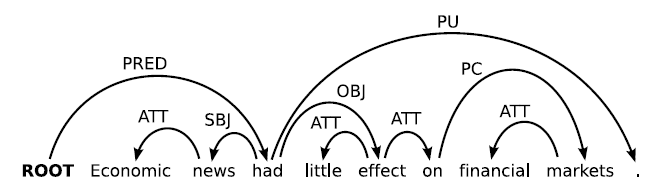
\includegraphics[scale = 0.6]{figures/dep-tree.png}
    \centering
    \caption{Dependency parsing tree~\cite{kubler2009dependency}}
    \label{fig:depParsetree}
\end{figure*}

Part of speech (POS) tagging refers to finding part of speech tags (e.g., nouns, verbs, adjectives) in a sentence. Often POS tagging is a precursor step in parsing, which is why, I look at POS tagging in my experiments, as well. These tasks generally work well when applied on the dataset from the same domain. However, the performance suffers when source and target are from different domains. The work in the area is largely driven by unavailability of data from the target domain. It is nearly impossible to hand annotate the huge amount of data generated by various sources. Manual annotation is even harder when the syntactic structure of the data differs widely. E.g., the syntactic structure of a newspaper corpus is very different from that of social media or academic journals from biomedical domain or literary works. This is an interesting problem since a deep understanding of syntactic structure of a sentence helps in variety of NLP tasks such as question answering, sentiment analysis, opinion mining, etc. Dependency parsing is particularly useful because the dependency relations serve as an important feature to detect negation or multi word expressions, for instance. 


%%%%%%%%%%%%%%%%
% Chapter 2 - Methodology
%%%%%%%%%%%%%%%%

\chapter{Methodology}
\todo[inline]{POS tagging; Dependency Parsing ; TM; TBL}

%\atrcomments{TBD!!!!!}




% \begin{enumerate}[label=Setting \arabic*,leftmargin=*]
% %\setlength\itemsep{2pt}
%     \item We consider all the sentences set aside as the test set has incorrect dependency labels.
%     \item Test set contains a mix of sentences with correct and incorrect dependency labels. 
% \end{enumerate}




\section{Topic Modeling}

Probabilistic topic modeling is a class of algorithms which detects
the thematic structure in a large volume of documents. Topic modeling
is unsupervised, i.e., it does not require annotated
documents \cite{Blei:2012:PTM:2133806.2133826} but rather discovers similarity between documents. Latent Dirichlet
Allocation (LDA) is one of the topic modeling algorithms. It is a
generative probabilistic model that approximates the underlying hidden topical structure of a collection of texts based on the distribution of words in the documents \cite{Blei:2003:LDA:944919.944937}. I explain LDA in more detail below.

\paragraph*{LDA} 

Intuitively, Latent Dirichlet Allocation (LDA) is a method for discovering the hidden topics in a sentence. E.g., consider the following WSJ sentence. If we choose to model this in terms of LDA, we get the output shown in table~\ref{tab:2topicssent} and \ref{tab:10topicssent}.


``Though growers can't always keep the worm from the apple , they can protect themselves against the price vagaries of any one variety by diversifying -- into the recently imported Gala , a sweet New Zealand native ; the Esopus Spitzenburg , reportedly Thomas Jefferson's favorite apple ; disease-resistant kinds like the Liberty."
 
 % Please add the following required packages to  document preamble:
%\usepackage{multirow}
\begin{table*}[!htb]
\centering

\caption{2 topics distribution}
\begin{tabular}{cc}
%\multicolumn{2}{c}{2-topic probability distribution} 
\\ \hline
0 & 1 \\
95.90 & 4.10 \\ \hline
\end{tabular}
\label{tab:2topicssent}

\caption{10 topics distribution
%\\ 
}
\begin{tabular}{cccccccccc}
%\multicolumn{10}{c}{10-topic probability distribution} 
\\ \hline

0 & \multicolumn{1}{c}{1} & \multicolumn{1}{c}{2} & \multicolumn{1}{c}{3} & \multicolumn{1}{c}{4} & \multicolumn{1}{c}{5} & \multicolumn{1}{c}{6} & \multicolumn{1}{c}{7} & \multicolumn{1}{c}{8} & \multicolumn{1}{c}{9} \\
0.11 & 0.10 & 0.08 & 0.10 & 0.09 & 30.58 & 15.28 & 49.55 & 3.93 & 0.16 \\ \hline
\end{tabular}
\label{tab:10topicssent}

%\caption{2 \& 10-topic probability distribution for a WSJ corpus sentence: \\ }
%\label{tab:10t-probab}
\end{table*}

I.e., when we choose the number of topics as 2 \& 10, LDA creates a probabilistic distribution of topics in the sentence. This process of discovering topics in a document can be represented by a generative model. Figure~\ref{fig:ldaplate} shows the plate diagram for graphical model for LDA. Plate diagrams are standard for representing repeating entities in a graphical model for Bayesian inference. Each document($W$), i.e., a sentence in this case, is a mixture of topics. In other words, a sentence consists of a collection of words, i.e., $W = {w_1,w_2, ..., w_N}$. A corpus can be represented as a collection of $M$ sentences or documents, i.e., $C = {W_1, W_2, ..., W_M}$. For each sentence in a corpus, the generative steps for LDA can be given as below:
\begin{itemize}
    \item The number of words in a sentence i.e., $N$ is chosen from a Poisson distribution.
    $$N \sim Poisson(\lambda)$$
    \item The mixture of topic for a sentence is chosen according to the dirichlet distribution over a fixed set of topics.
    $$\theta \sim Dirichlet(\alpha)$$
    \item Each word ($w_i$) in sentence ($W$) can be generated as follows:
    \begin{itemize}
        \item Pick a topic according to the multinomial distribution sampled above.
        $$Z_n \sim Multinomial(\theta)$$
        \item Generate the word from the topic according to the multinomial distribution of topics. I.e., we choose a word from $p(w_n|Z_n, \beta)$, where $\beta$ represents word probabilities.
    \end{itemize}
    
    
\end{itemize}

The inference/parameter estimation step follows the generative step, which requires calculating the posterior distribution of the hidden variables given a sentence. 
\atrcomments{to be finished ........}




\begin{figure*}[t]
    \centering
    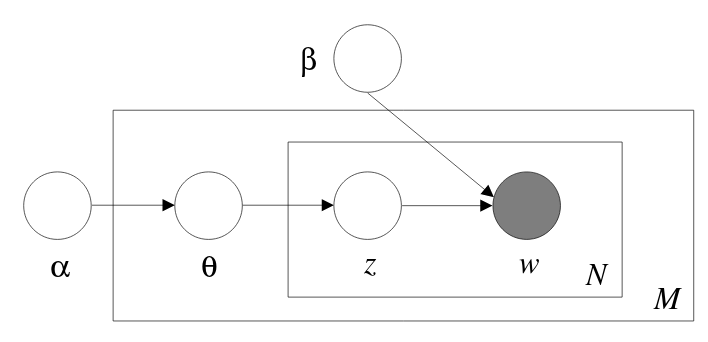
\includegraphics[width=\textwidth]{figures/LDA_plate_diagram.png}
 \caption{Graphical model for LDA~\citep{Blei:2003:LDA:944919.944937}}\label{fig:ldaplate}   
 \end{figure*}
 

\paragraph*{LDA toolkit}

There are several  open sourced toolkits available for LDA. We use the topic modeling toolkit MALLET \cite{McCallumMALLET}.  The
topic modeler in MALLET implements Latent Dirichlet Allocation (LDA), clustering
documents into a predefined number of topics. As a result, it provides
different types of information such as:

\begin{itemize}
	\item  Topic keys:  The highest ranked words per topic with their probabilities; 
	
	\item Document topics: The topic distribution for each document (i.e., the probability that a document belongs to a given topic); and 
	
	\item Topic state: This correlates all words and topics.
	
\end{itemize}

\section{POS Tagging}

Part of speech (POS) tagging refers to assigning part of speech tags, which can also be referred to as word class (e.g., nouns, verbs, adjectives) in a sentence. This is an interesting problem since a deep understanding of syntactic structure of a sentence helps in variety of NLP tasks such as question answering, sentiment analysis, opinion mining, etc. Often POS tagging is a precursor step in parsing, which is why, I look at POS tagging in my experiments, as well. Figure~\ref{fig:postag} shows a part-of-speech tagged sentence.

\begin{figure}[t]
    \centering
    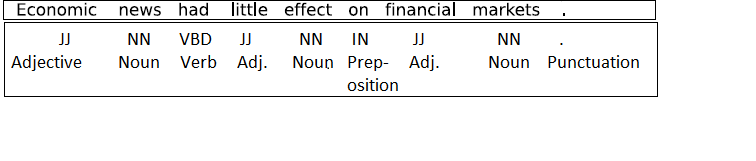
\includegraphics[scale = 0.9]{figures/postagging.png}
    
    \caption{An example of POS tagging}~\label{fig:postag}
\end{figure}

As shown in the figure~\ref{fig:postag}, the task of POS tagging involves classifying words into their corresponding classes such as nouns, verbs, adjectives, etc. The most widely used POS tagset is the Penn Treebank tagset~\citep{Marcus:1994:PTA:1075812.1075835}. It contains 45 POS tag classes. Most of the available corpora use the PTB tagset with some variations. Availability of a tagged corpora is essential for corpus driven POS tagging. 

Broadly, POS tagging can be rule-based~\todo{cite papers cited by Brill}, transformation-based~\citep{brill1992simple} and stochastic. I discuss the process of transformation based error driven POS tagging in greater detail in section~\ref{sec:TBL}. The problem of supervised stochastic part of speech (POS) tagging has been addressed by using generative models such as Hidden Markov Models (HMM)~\citep{brants:00.2} and  discriminative models such as Maximum Entropy Markov Model (MEMM)~\citep{ratnaparkhi1996maximum}. More recently, the deep learning based sequence modeling techniques have gained prominence.~\todo{cite}. %Since I use TnT tagger for my experiments, I will delineate the steps involved in HMM-based POS taggers. 
I use the TnT (Trigrams'n'Tags) tagger~\cite{brants:00.2} for part of speech tagging experiments. TnT is based on a second order Markov Model and has an elaborate model for guessing the POS tags for unknown words. I use TnT mainly because of its speed and because it allows the manual inspection of the trained models (emission and transition frequencies).

POS tagging is essentially a sequence labeling task. I.e., given a sequence of words, the problem is to determine the most likely POS tags for the sequence. HMMs are widely used in sequence labeling tasks. These are probabilistic sequence models that take into account that there are observed and hidden events influencing the probability of a sequence. In case of POS tagging, as shown in figure~\ref{fig:postaghmm}, the observed events are words and POS tags are the hidden events.

\begin{figure}[t]
    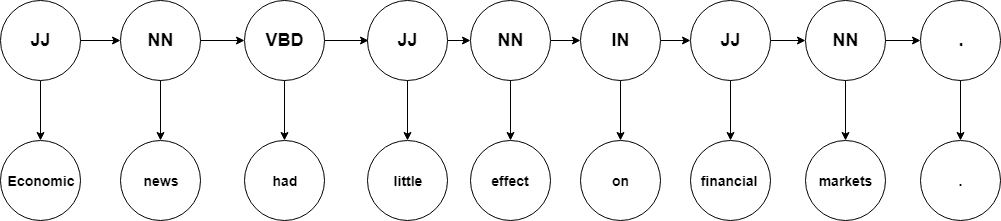
\includegraphics[scale = 0.45]{figures/hmmpos.png}
    \caption{POS tagging as HMM}~\label{fig:postaghmm}
\end{figure}

Typically an HMM has two parts - emission probabilities and transition probabilities. For POS tagging, the transition probability is the probability of encountering a POS tag given the POS tag at previous time point i.e.,  $P(t_i|t_{i-1})$. The emission probability computes the probability of affiliation of a word with a POS tag at a certain state, i.e., $P(w_i|t_i)$. These probabilities are calculated using maximum likelihood estimates (MLE) as given below.

\begin{align}~\label{eq:transprob}
    P(t_i|t_{i-1}) = \frac{Count(t_{i-1},t_i)}{Count(t_{i-1})} 
\end{align}

\begin{align}~\label{eq:emprob}
    P(w_i|t_i) = \frac{Count(t_i,w_i)}{Count(t_i)}
\end{align}
    
The problem, then is to compute the most probable sequence of hidden variables, i.e., POS tags given the observaions, i.e., the words. This is also known as decoding. TnT calculates this by using a second order Markov model, which means that instead of using bigram probabilities as shown in~\ref{eq:transprob}, it uses trigram transition probabilities. Therefore, the most probable tag sequence for a sequence of length $N$, is calculated as:

\begin{align}
    \hat{t} = \underset{t_1 ... T_N}{argmax}  \bigg [ \prod_{i=1}^N P(t_i|t_{i-1},t_{i-2}) P(w_i|t_i) \bigg] P(t_{N+1}|t_N)
\end{align}

To account for data sparsity - not all trigrams have equal representation in the training dataset - smoothing is applied. In TnT, a context independent linear interpolation of $n$-grams is used for smoothing.

\begin{align}
    P(t_i|t_{i-2},t_{i-1}) = \lambda_1 \hat{P}(t_i|t_{i-2},t_{i-1}) + \lambda_2 \hat{P}(t_i|t_{i-1}) + \lambda_3 \hat{P}(t_i)
\end{align}
where, $$\sum_{i=1}^3 \lambda_i = 1$$
and $\hat{P}$ estimates the MLE estimates. The bigram estimate is shown in equation~\ref{eq:transprob}. The unigram and trigram MLEs are given below:

\begin{equation}
    \hat{P}(t_i|t_{i-2},t_{i-1}) = \frac{Count(t_{i-2},t_{i-1},t_i)}{Count(t_{i-2},t_{i-1})}
\end{equation}

\begin{equation}
    \hat{P}(t_i) = \frac{Count(t_i)}{N}
\end{equation}



The values of $\lambda$ are estimated using deleted interpolation~\citep{jelinek1980interpolated}. 
In TnT, the unknown words are estimated using suffix analysis following the work by~\cite{W93-0420}. Additionally, probability distribution of words around capitalized words contributes further to the disambiguation process.~\todo{detail?} 

The most likely subsequence of tags is generally computed using Viterbi's Algorithm. This is a dynamic programming approach which operated by first computing the probability matrices given the previous observations. Finally the sequence with the highest path probability is selected as the final sequence.~\todo{I think I need to detail?} 
However, depending on the length of the sentence, the time complexity for Viterbi algorithm can be quadratic. To improve this, beam search is applied. Hence, for each time step, the decoding process now considers the best $n$ hypotheses pruning the rest. TnT implements this to achieve better time complexity than regular Viterbi. 

\todo[inline]{Should I describe MEMMs too? also CRF taggers?}






%These tasks generally work well when applied on the dataset from the same domain. However, the performance suffers when source and target are from different domains. The work in the area is largely driven by unavailability of data from the target domain. It is nearly impossible to hand annotate the huge amount of data generated by various sources. Manual annotation is even harder when the syntactic structure of the data differs widely. E.g., the syntactic structure of a newspaper corpus is very different from that of social media or academic journals from biomedical domain or literary works.  Dependency parsing is particularly useful because the dependency relations serve as an important feature to detect negation or multi word expressions, for instance. 


%\paragraph*{POS Tagging Toolkit}



\section{Dependency Parsing}\todo[inline]{to be fixed}

Syntactic parsing refers to the process of extracting and analyzing the syntactic structure or representation of a natural language text. This is very useful is a variety of different domains such as machine translation, information retrieval, question answering \cite{hall2008transition}. More formally, we can define it as a structural prediction problem. Hence, there is an input which are sentences; an output, which are syntactic representation of a sentence;  and a model that maps the input to the output. The input sentence is usually split into tokens. The output is represented as trees. Dependency parsing is a type of syntactic parsing analyses the dependency structure of a sentence based on a dependency grammar. As illustrated in figure~\ref{fig:depParsetree}, the words in a sentence are linked with relations (shown using labeled arrows), also known as dependency relation (dependencies) where one word is the dependent~\footnote{can also be referred to as child} which depends on the head~\footnote{can also be referred to as parent}. In order to simplify the problem to provide a syntactic head to the word which does not have a head, an artificial root is introduced~\cite{kubler2009dependency}. Dependency parsing gained prominence because of the flexibility it provides for free word order languages such as Czech.

Most commonly used dependency parsing approaches are transition-based and graph-based. The transition based approach is a greedy locally optimized classifier that learns how to get from one parse state to the next. %For dependency parsing, each step represents the steps for deriving the final dependency tree. These are stack-based and there are usually three different kinds of transitions - shift, left \& right which are chosen based on an oracle, usually a machine learning classifier such as SVM. 
In contrast, for graph-based dependency parsing, the problem lies in finding maximum spanning trees (MST). The MST parser is state of the art in graph based parsing. The core idea of the parser to compute a score of the dependency tree~\footnote{Score of the tree is the sum of the score of each edge of the tree} which is a dot product of weight and a high dimensional feature vector. %Thus, it can be thought of as a problem of multiclass classification, where each dependency tree of the sentence is a class. 
The resulting dependency parse is the highest scoring tree. I use MATE~\cite{bohnet2010very}~\footnote{code.google.com/p/mate-tools} which is a reimplementation of MST parser~\cite{McDonald:2005:NDP:1220575.1220641} for my experiments. %MATE parallelizes the feature extraction and parsing algorithm by using passive-aggressive perceptron algorithm~\cite{crammer2006online} as Hash Kernel. 
The parser is highly efficient in terms of memory utilization and CPU requirements while maintaining the accuracy of the resultant parses.
%Bohnet reported a 3.5 times increase in speed over the baseline MST parser using a single core CPU and it also requires a lot less memory than the contemporary parsers by using Hash Kernel. The speed increases further by using parallel algorithms and it can be further reduced at the cost of accuracy.

\begin{figure*}[!htb]
    \centering
    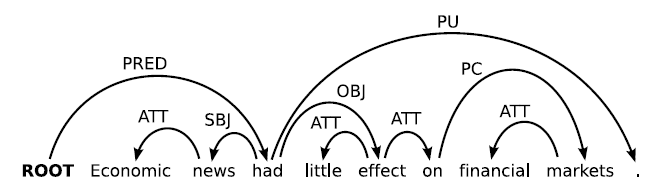
\includegraphics[scale = 0.6]{figures/dep-tree.png}
    \centering
    \caption{Dependency parsing tree~\cite{kubler2009dependency}}
    \label{fig:depParsetree}
\end{figure*}

\todo[inline]{this is from the qual paper}
The process of automatically analyzing dependency structures to an input sentence is referred to as dependency parsing. A dependency tree needs to satisfy the following properties~\cite{kubler2009dependency}:
\begin{itemize}
\item A dependency tree needs to have an artificial root which specifies that there there must not exist an arc which comes into the root from another node(word).
\item A dependency tree must satisfy the spanning property for all the words in a sentence.
\item A dependency tree must be connected i.e., if we ignore the directed edges then every word in a sentence must be connected.
\item Every word in the dependency tree must have one head only.
\item A dependency tree must be acyclic, i.e., should not contain cycle.
\item Number of arcs in the dependency tree must be one less than the number of words, i.e., $$|E| = |W| - 1$$ for a dependency tree $G = (W,E)$ where E is number of arcs and W is number of words.
\end{itemize}

There are two different kinds of dependency structures based on which, dependency trees can be categorized into two types. Figure~\ref{fig:proj-non-proj} shows an example illustrating the difference between projective (right) and non-projective (left) trees.  

\begin{figure*}[!htb]
    \centering
    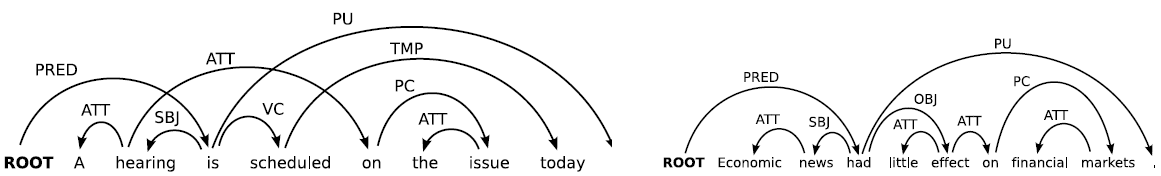
\includegraphics[scale = 0.45]{proj-non-proj.png}
    \centering
    \caption{Projective and Non-projective dependency trees~\cite{kubler2009dependency}}
    \label{fig:proj-non-proj}
\end{figure*}

\begin{itemize}
    \item Projective dependency trees - For these dependency trees, the dependencies do not cross each other. Usually, the sentences in English are projective.
    \item Non-projective dependency trees - For these type, the dependency branches can cross each other. This is more prevalent in the languages with free word order like German.
    
\end{itemize}


There are two major approaches for this problems - data-driven and grammar-based. The grammar-based approaches make use of a formal grammar and the problem in this case is defined as - whether the input sentence belongs to the language defined by this formal grammar. In contrast to grammar-based approaches, data-driven approaches utilize machine learning approaches on annotated data from a corpus to parse a given input sentence. Since data-driven approaches rely on machine learning approaches, we will only discuss these methods in the rest of the report.

\begin{itemize}
    \item{Transition-based - }{In a transition-based approach are based on the notion of transition system which is a finite state automaton. An FSA consists of states, transitions, mapping states and input symbols and transitions from initial to final states. The state transition happens on an input to a state. In case of transition based parsing, each of the states represent steps for deriving a dependency tree. These approaches make use of a stack-based technique for parsing. Transition based systems are mostly stack-based. Initially, the stack contains the artificial root and the buffer is empty. There are three kinds of transitions - shift, left and right. This is a bottom-up approach, i.e., for an arc to be constructed between two nodes, it is imperative that the dependent node has already a dependency tree constructed. This approach is also known as arc-standard. There is another approach called arc-eager where the terminal configuration is guided by the state of the buffer. If it is empty the arc-eager system terminates. In addition to the transitions in the arc-standard system, there is an additional transition called reduce. This is a top-down parsing approach as the arcs are added as and when found~ \cite{kubler2009dependency}.
    }
    \item{Graph-based - }{Graph-based approaches rely on the algorithms for directed graphs like finding the maximum spanning trees. There is a scoring function which evaluates how correctly a particular tree analyzes a sentence~\cite{kubler2009dependency}. }
\end{itemize}
 
Various machine learning techniques have been implemented in different stages of parsing. In general, machine learning algorithms are used to compute scores in case of graph-based algorithms while for transition-based systems, it is used as an oracle. Supervised learning methods have proven useful while most recently, semi-supervised and unsupervised methods have shown promise. The goal is to reduce the time taken in parsing while not compromising the quality of the parse. 
The parsing problems by using these approaches are discussed in further details in the subsequent sections. We have further sub-categorized problems by whether they work for projective or non-projective sentence structures. Usually, the problem with projective sentences are a subclass of that of the non-projective sentences. The pseudo-projective approaches are also listed under the non-projective approaches. Neural network approaches are categorized in a separate section for ease of readability.

%\subsection{Discriminative Models}
\subsection{Transition based approaches}

Broadly, there are two main approaches to transition based parsing. 

\begin{itemize}
\item Greedy classifier based - The transition-based approach has a set of transitions between the states (or configuration). However, to categorize this as a parsing problem, we need to score these transitions and estimate the highest scoring transition by using a model. A classifier can be used as this model which maps configurations to the most optimal transition. The optimal transition can be determined in a greedy way, where the final optimal transition is determined by selecting the optimal transitions locally. A representation of the scoring is as below:
\begin{equation*}
Score(C, T) = \sum_{i = 1}^{N} f_i(C,T).w_i
\end{equation*}
where C = configuration, T = transition
Many machine learning techniques are used to learn the weights such as SVMs, perceptrons, etc.(more recently, neural networks)

\item Beam search and structure learning - The beam search and structure learning has a similar strategy, however, in this case, instead of a greedy search, beam search is applied. Thus instead of 1 optimal transition, $n$ number of possible optimal solutions are considered at each step where $n$ is the beam size. The second part is similar to greedy classifier method, except that it has been seen (as we will see later in this chapter) that structured learning approaches tend to have better results.
\end{itemize}

We discuss the existing methods for transition based learning from the point of view of projectivity. Since our objective is to highlight the machine learning approaches, we will look at it from the perspective of the machine learning techniques used.

\subsubsection{Projective}

Probabilistic approaches to parsing initially showed promising results in dependency parsing as compared to rule-based techniques. 
%A simple bigram probabilities estimation technique was used to estimate the probability of dependencies between pair of words for the Wall Street Journal corpora~\cite{Collins:1996:NSP:981863.981888}. 
%Decision trees~\cite{haruno1999using} and Maximum Entropy models~\cite{Charniak:2000:MP:974305.974323} were also implemented for dependency structure analysis. However, these approaches did not address the feature selection or in other words, how selecting good features could be a key in improving the results in dependency structure analysis. So, 
Previous work in syntactic parsing (constituency parsing, in most cases) did not address the feature selection or in other words, how selecting good features could be a key in improving the results in dependency structure analysis.
So, Kudo and Matsumoto\cite{Kudo:2000:JDS:1117794.1117797} applied Support Vector Machines (SVMs) for analysis of dependency structure in Japanese. They assume that the dependency structure holds the following constraints.
\begin{itemize}[leftmargin=*]
\itemsep-0.5em
    \item Each item depends on exactly one item appearing to the right.
    \item The dependencies are projective.
\end{itemize}
Since, the problem of statistical dependency analysis deals with finding the best dependency structure($D_{best}$) given a sequence of chunks of a sentence ($B$) (chunks are specific to Japanese dependency structure and are defined as relation between phrasal units), it can be formulated as follows:
\begin{equation*}
    D_{best} = \arg\max_{D} P(D|B)
\end{equation*}
Considering the dependent probabilities are independent of each other, $P(D|B)$ can be written as:

\begin{equation}
P(D|B) = \prod_{i=1}^{m-1}P(Dep(i)=j|f_{ij}) 
$ where, $ 
f_{ij} = {f_1,...,f_n} \in R^n 
\end{equation} \\
$P(Dep(i)=j|f_{ij})$ denotes the probability that the chunk i depends on the chunk j given an n-dimensional linguistically-motivated feature set. 
To find $D_{best}$, the authors have used the backward beam search technique for statistical dependency analysis of Japanese sentence by~\cite{Sekine:2000:BBS:992730.992755} which processes a sentence backwards.

The feature set consists of static features such as, head words and their parts-of-speech, particles and inflection forms of the words appearing at the end of chunks, distance between two chunks, existence of punctuation marks. In order to handle long sentences, dynamic features are included which resolves syntactic ambiguity at the time of parsing. These are mainly ``form of functional words or inflection that modifies the right chunk". The authors report a better accuracy compared to the previous work on the same corpus.

A similar discriminative model for dependency analysis on Wall Street Journal section (02-21 for training and 23 for test) of the Penn Treebank~\cite{Marcus:1994:PTA:1075812.1075835} using SVMs by Yamada and Matsumoto\cite{yamada2003statistical}.  They apply a deterministic bottom-up parsing algorithm which comprises of three actions - \textit{Shift}, \textit{Left} and \textit{Right}. The parsing algorithm undergoes a two-step procedure to parse an input sentence considering words from left to right. The first procedure involves assessing the appropriate action (\textit{Shift} or  \textit{Left} or \textit{Right}) from the contextual information provided by the surrounding words. Then, the parser builds the dependency tree by executing these actions determined in the previous step. During the training phase, each sentence is parsed using this algorithm. The contextual features with the right parsing action serves as an example for the SVM. Thus the estimation phase is a multiclass classification problem comprising of three binary classifiers for each action in a pairwise fashion:
\begin{itemize}[nolistsep,leftmargin=*]
%\itemsep-.75em
\item Left vs. Right
\item Left vs. Shift
\item Right vs. Shift
\end{itemize}
The decision on the action that needs to be implemented at any stage is determined by the cumulative votes from each of these SVMs. 
The features are as follows:
\begin{itemize}[nolistsep,leftmargin=*]
%\itemsep-.25em
\item word
\item Part of Speech (POS) tags
\item child word modifying the parent node on the right hand side
\item child word modifying the parent node on the left hand side
\item POS tag of the child node modifying the parent node on the right hand side
\item POS tag of the child node modifying the parent node on the left hand side
\end{itemize}
Each feature is defined as a triplet consisting of the position from target node, feature type and the feature value. The accuracy of this parser is not at par with the contemporary phrase structure parsers owing to the fact that the phrase structures are not utilized in this parser. Malt parser (discussed in the non-projective section) addressed the problems faced by this parser viz., requirement to iterate for long sentences.

Cheng~\etal~\cite{cheng2005chinese} applied a similar approach using SVMs to determine if a dependency relation exists for any two pair of words based on  Chinese Treebank. The parsing method is based on Nivre and Scholz's~\cite{Nivre:2004:DDP:1220355.1220365} bottom-up deterministic algorithm which parses a sentence in linear time. The basic difference is in the machine learning algorithm used for these two papers. While Nivre and Scholz used memory based learners ($5$-nearest neighbors (IB 1) from TiMBL~\cite{daelemans2004timbl}). This algorithm is also stack-based, where the analyzer states are represented as a triple $\langle S, I, A \rangle$ where $S$ contains the words which are being considered, $I$ contains the words which are to be processed and $A$ is a list of dependency relation. 
It is also important to point out the differences between Yamada and Matsumoto's approach to that of Nivre's since both are based on English text and use a deterministic parsing algorithm. The primary difference would be the choice of classifiers, SVMs vs. MBL. Yamada and Matsumoto's parser requires multiple passes but Nivre's take one pass which makes Yamada's algorithm's worst case time complexity to be quadratic as compared Nivre's algorithm's linear time.
The data-driven dependency parsing was further used for parsing Swedish~\cite{nivrej.2004}, Bulgarian~\cite{marinov2005data} and Turkish~\cite{eryiugit2008dependency} treebanks with improvement over baseline.

At any stage, there are four possible operations for a given configuration - right, left, reduce \& shift. Right \& left operations add dependencies based on whether the top word in $I$ depends on the top word in $S$ or in the other direction respectively. For reduce, if the top element of $S$ has no dependents, it is removed. For shift, the analyzer checks whether there is any possible dependency relation between the top elements of $S$ and $I$. If it does not find one and the conditions for reduce are not met as well, then the top element of $I$ is pushed into $S$.

Since the two methods (Cheng vs. Nivre) use different machine learners, the feature set is different. Nivre and Scholz considered the top word of the stack, the next input token, left and right dependent of the top element in the stack, left dependent of the next input token, the possible tokens from next configurations which are connected through a dependency arc. For the tokens in consideration, the lemma and part of speech tags are considered, while for the ``lookahead" tokens, they have only considered the part of speech tags. For Cheng's work, each node comprises of the word, POS tags and information of its children. They also take context features, such the preceding and succeeding nodes and its children into consideration. These are treated as local features. The global features are used for the long distance dependencies. If the local features arrive at a decision which is shift/reduce, the analyzer uses SVMs to determine the correct operation using global features. They have also proposed a two-step process for finding the root words using SVMs. They have reported an increase in accuracy by employing the global features and the root word finder. 

This method was further extended to account for multiword units (MWUs) such as multiword names, function words by Nivre and Nilsson~\cite{nivre2004multiword}. Particularly, to examine whether multiword units help in improving the parser results and if so, at which point should this be implemented. They experimented on the lexicalized and non-lexicalized versions of the parser based on memory-based learning. They show a significant improvement over the baselines for the syntactic structures in addition to the MWUs.

In order to analyze whether there is a ``better" machine learning algorithm for parsing, Hall~\etal~\cite{Hall:2006:DCD:1273073.1273114} presented a comparison between SVMs and memory based learning classifiers in deterministic dependency parsing for English, Chinese and Swedish using a variety of features. They show that the accuracy achieved by these classifier based models are almost at par with more complex parsing models. For their experiments, SVMs outperform the memory based learners but with a tradeoff in training times.

\paragraph{Pseudo projective approaches}

English sentences are generally projective, i.e., the edges of the dependency trees do not cross each other in a sentence. However, in the languages with a flexible word order like German, Czech and Dutch, the sentences tend to be non-projective with crossing dependencies. To solve, this problem, Nivre and Nilsson~\cite{nivre2005pseudo} devised a ``pseudo projective" method for parsing and reported an improvement over the state-of-the-art non-projective parsing results for Prague Dependency Treebank~\cite{bohmova2003prague,hajic1998building} by using a combination of data-driven deterministic dependency parsing (memory-based) with a graph transformation technique called lifting. Typically, a non projective dependency graph can be converted to a projective one by replacing the non-projective arc with a projective one. The authors have implemented a transformation involving a minimal number of lifts. Thus, at the first step, the dependency trees are projectivized by applying the minimal lift transformation technique. In the second step, they have implemented an inverse transformation based on the breadth-first search algorithm using three encoding schemes. As a part of the experiments, memory based dependency parsers are used and the projectivized trees are used for training. The output is transformed using the inverse transformation and compared to the gold standard test set.

\subsubsection{Non-projective}

While the parsing techniques for English have proven to be efficient enough, parsing non-projective tree structures can prove to be challenging. A lot of techniques, as we will see later for the generative models as well, work for non-projective sentences with some modification on the projective counterparts. 
          
This problem has been addressed by Nivre~\etal\cite{nivre2006maltparser,nivre2007maltparser}, who introduced MaltParser, which they describe as ``data-driven parser-generator for dependency parsing". The parser requires a treebank and not a grammar unlike contemporary parser-generators. The parsing comprises of - building dependency graphs by deterministic parsing algorithms as shown by Yamada and Matsumoto and Nivre, estimating the next action of the parser by building a history-based feature model and finally mapping the history to parser action using discriminative machine learning algorithms (as demonstrated in Yamada and Matsumoto's and Nivre's work) such as memory based learning, SVMs. MaltParser specifies a fized set of data structures and typically any parsing algorithm which follows this architecture would work in the framework. It supports Nivre's~\cite{nivre2003efficient}[An efficient algorithm for projective dependency parsing] and Covington's~\cite{covington2001fundamental} algorithms which uses three approaches - Brute-force search, Exhaustive left-to-right search and enforcing uniqueness. The feature models consists of word, lemma, part of speech tags, dependency type described in terms of the provided data structures. The evaluations provided by Nivre~\etal for MaltParser is for Swedish, English, Czech, Danish and Bulgarian based on memory based learning.

It is clear that, parsing accuracy and time is an issue for non-projective parsing, which caused largely due to the way non-projective dependencies are handled. Also, it has been argued that, even for the free word order languages, the dependency structures tend to be either projective or ``very nearly projective". This leads to the discussion of finding the appropriate ``degrees of non-projectivity"~\cite{nivre2006constraints}, which can be stated as finding a balance such that a small amount of non-projectivity might improve the parsing accuracy and time over strict projectivity and it is also more efficient than considering non-projectivity in abundance. Nivre~\cite{nivre2007incremental} investigated this appropriate degree of non-projectivity by using Covington's parsing algorithm with history based SVM classifier to  predict the next parser action. The results indicate that the languages exhibiting extensive non-projectiveness, the parser accuracy can be boosted if the non-projective dependencies are derived. However, on the other hand, parsing times can be improved by curbing the non-projectivity with a small decrease in parsing accuracy. 

Although SVMs work well in case of parsing, it can be expensive in terms of training and memory requirements. A better workaround for this can be, to use multi layer perceptrons as the classifier~\cite{attardi2009accurate} as perceptrons are faster and require less memory.  



%\cite{bohnet2010very}

%A Transition-Based System for Joint Part-of-Speech Tagging and Labeled Non-Projective Dependency Parsing

%Getting the Most out of Transition-based Dependency Parsing

%Transition-based Dependency Parsing with Rich Non-local Features


%\subsection{Generative Models}

\subsection{Graph based approaches}

The most basic model for graph based parsing is the arc-factored model. An arc is an edge in the dependency tree. This is also commonly referred to as the first order model since the score is computed based on the scores of each arc. This is an exact inference. However, research has indicated that better parsing accuracy can be achi  eved when we considered bigger subgraphs i.e., set of 2 or 3 arcs in dependency tree. These models are referred to as second and third order models respectively but it increases the parsing complexity i.e., for learning and parsing. These are approximate inferences. In the subsequent sections, we have divided graph-based models in terms of projectivity and non-projectivity. 



\paragraph*{Eisner's Algorithm}
Quite a lot of work has been done using generative models to improve the results of dependency parsing. To address the ``lexical blindspot" of context-free grammars (CFGs), Eisner~\cite{eisner1996three} proposed three different probabilistic approaches to describe the basic structure of a sentence and apply it to a dependency framework for improving the resulting parses. This is a constituent CKY based algorithm for dependency parsing which uses words as node labels. This has been used for parsing projective dependencies The probabilistic models are as follows:

\begin{figure*}[!htb]
    \centering
    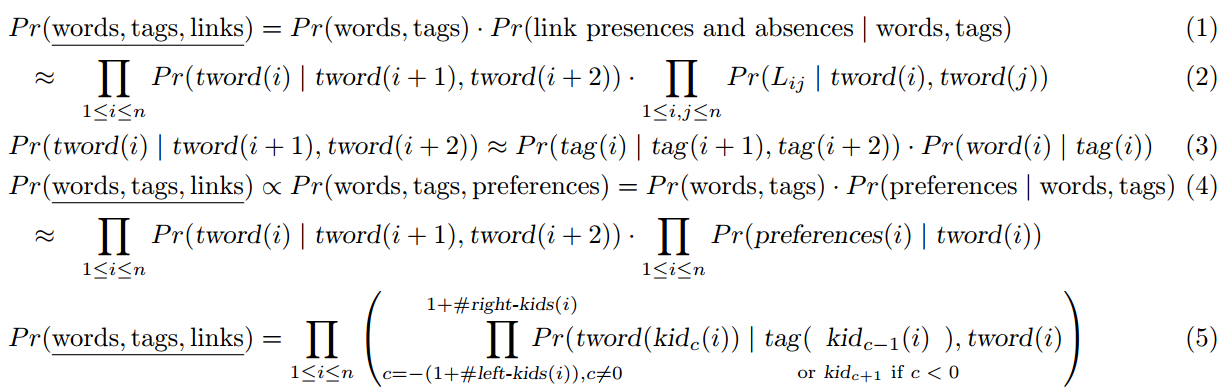
\includegraphics[scale = 0.45]{Eisner.png}
    \centering
    \caption{Three probabilistic models in Eisner's work}
    \label{fig:eisnerexpressions}
\end{figure*}

\begin{itemize}

\item Bigram lexical affinities [expressions 1-3 in Fig.~\ref{fig:eisnerexpressions}]

The first step is to generate tags by a Markov process given the previous two tags. Next, a word is chosen, given each tag. To account for the dependencies, there is a third step in this process which considers pairs of words and makes a random decision whether to link the two based on whether the probability of the words being linked together is ``lexically sensitive". I.e., both the tag and word are considered for any pair of words. This model also accounts for the inter-dependencies between the children of a word.

\item Selectional preferences [expressions 4 in Fig.~\ref{fig:eisnerexpressions}]

A sequence consisting of word and its tags are generated by a Markov process and then for each word, a parent is described. Hence the ``selectional preference"\footnote{referred to as disjunct, in the paper} for each word is being considered in this case. Then, each of the words are independently ``sense tagged" based on its selectional preference.

\item Recursive generation [expressions 5 in Fig.~\ref{fig:eisnerexpressions}]

This is a generative model as opposed to the two previously described comprehensive models. Every time a word is added, two separate Markov sequence of tag/word pairs are generated to serve as its left and right children. This process continues recursively for each child which is generated.

\end{itemize}

A probabilistic algorithm which is similar to CKY is proposed as the parsing algorithm. CKY considers substrings of increasing length for parsing and thus each such substring is represented as lexical trees. But, in this case, instead of considering substring as trees, the parser considers these as spans. These approaches when tested on the WSJ corpus indicate that the recursive generation model performs better as compared to the other two. The parsing algorithm has a $O(n^3)$ complexity. 

Training these models is particularly easy as it constitutes mainly of estimating probabilities by counting the events related to parsing in the training set. However, this advantage is sometime nullified due to the poor decisions in the independence assumptions. This is where the discriminative models tend to perform better. However, these especially Maximum Entropy Markov Models based parsers~\cite{ratnaparkhi1999learning} tend to run into the label bias problem (\atrcomments{?}) because it does not take the parsing decisions based on an observation which might be seen later in the sequence. Parsing the training corpus repeatedly can solve this problem to some extent. However, it is really expensive - $O(n^5)$ as opposed to $O(n^3)$ for generative models. Hence, to strike a balance and utilize reduced parsing complexity of generative models like Eisner's, McDonald~\etal~\cite{McDonald:2005:OLT:1219840.1219852} described a method of training dependency parsers for English and Czech using margin-sensitive online training algorithms~\cite{crammer2003ultraconservative,shalev2003online}. The authors mention that this method can be translated for non-projective cases (where it may appear in Czech, for instance) as well. Since the reported results are for projective cases only, we have listed it so.



\paragraph*{Chu-Liu-Edmonds Algorithm}

Chu-Liu-Edmonds algorithm\cite{chu1965shortest,edmonds1967optimum} often serves as a basis for non-projective parsing approach which determines the maximum spanning tree (MST) of a graph in a greedy and recursive way. We will informally explain the intuition behind the algorithm as follows:
\begin{itemize}[label={--}]
\item{Motivation: } All the nodes in a graph need to be in arborescence. I.e., there should be exactly one directed path between two nodes in the graph.
\item An incoming edge is selected for a node in a greedy way.
\item The highest scoring incoming edge is stored for every non-root node.
\item If a cycle is formed, a decision has to be made to remove one of the nodes to resolve the cycle. 
\item There are two stages - contract and expand. 
\item Following steps are followed for contract phase:
\begin{itemize}[label=$\diamond$]
\item At first, the nodes in a cycle are contracted to form a new node/vertex.
\item All the incoming edges to the nodes in the cycle are now redirected to the new node.
\item Similarly, the outgoing edges have the new vertex as its starting vertex.
\item  The incoming and outgoing edge weights for this new ``contracted" vertex are recalculated.
\item This process is repeated recursively until every non-root vertex contains exactly one incoming node and there are no cycles.  
\end{itemize}
\item The MST formed on this contracted graph can be shown to be equivalent to MST for the original graph. \cite{georgiadis2003arborescence}
\item Thus the algorithm is recursively implemented on the new graph to find the MST.
\end{itemize}


\paragraph{Non-projective approaches}
While the graph transformation techniques yielded good results with a cubic complexity, the parsing complexity was reduced by McDonald~\etal~\cite{McDonald:2005:NDP:1220575.1220641} who proposed a dependency framework for both projective and non-projective dependency parsing by formalizing the problem as searching for maximum spanning tree (MST). They have used a similar approach as Hirakawa's~\cite{hirakawa2001semantic} spanning tree search for dependency parsing. However, the worst case performance is exponential in this case as branch and bound algorithm is used. They used Eisner's spanning trees approach for projective and Chu-Liu-Edmonds algorithm~\cite{chu1965shortest,edmonds1967optimum} for non-projective dependency trees. At first, an edge-based factorization is applied to the projective languages with Eisner's parsing algorithm and Chu-Liu-Edmonds maximum spanning tree algorithm for non-projective languages. The edge factorization for an edge is done by computing a dot-product between a high dimensional feature representation of the edge in consideration and a weight vector. The score of a dependency tree is then a sum of the scores of all edges in the tree. The weight is updated by using the online learning algorithm implemented in McDonald~\etal~\cite{McDonald:2005:OLT:1219840.1219852}. Their results show significant improvement in accuracy even with a small amount of non-projective sentences. They also reported improved parsing times - $O(n^2)$ as compared to $O(n^3)$ - in favor of the Chu-Liu-Edmonds algorithm as opposed to Eisner's. Their parser performs well even when compared to state-of-the-art\atrcomments{?} lexicalized phrase structure parsers such as 
Collins~\etal~\cite{collins1999statistical} and Zeman~\cite{zeman2004parsing}, whose parsing complexity is $O(n^5)$. This framework was further account for higher-order feature representation and acyclic dependencies, i.e., multiple heads for each word~\cite{mcdonald2006online} by using approximate inferencing of the online learning algorithms. The defined approximation is to start with a reasonably good baseline structure and then continue making transformations until the structure converges. 

In order to devise more effective ways of solving multilingual parsing problems, McDonald~\etal~\cite{McDonald:2006:MDA:1596276.1596317} proposed a two-stage multilingual parser and evaluated it on the 13 language treebanks provided in different CoNLL shared tasks~\cite{Buchholz:2006:CST:1596276.1596305}. The first stage in this model is to create an unlabeled parse for an input sentence. They extend the existing models by McDonald \& Pereira~\cite{mcdonald2006online}, adding morphological features (where available) for each token. The morphological features (includes features for parent and its dependent and also various conjunctions of features from each of sets. The second stage is label classification which takes the output parse from stage 1 and assigns each edge with a label with the highest score. A first order Markov factorization has been used. Each factor is defined as the score of labeling adjacent edges. As defined in the earlier work by McDonald~\etal, the score function is defined as the dot product between the high dimensional feature representation and a weight vector. The most likely sequence of labels is then  ascertained by applying Viterbi's algorithm.


%paper= Online Large-Margin Training of Dependency Parsers

\paragraph{Higher order models}

As explained before, first order model is one in which the dependency tree os split into head and modifier dependencies. Second order models look into the adjacent dependencies in addition to these primary dependencies. McDonald \& Pereira~\cite{mcdonald2006online} experimented with second order graph models. Carreras~\cite{carreras2007experiments} extended this to experiment with other types of second-order relations. In particular, they look into PP-attachment which requires looking into grand parent relations. The training is done with averaged perceptron on Eisner's(1996) algorithm. Although it reported one of the best reported labeled attachment scores for some languages, this model suffers in terms of time and memory utilization. Bohnet~\cite{bohnet2010very} used this parser as a basis for their work on parallelizing the feature extraction and parsing algorithm by using passive-aggressive perceptron algorithm~\cite{crammer2006online} as Hash Kernel. The concepts from this model can be extended to the transition based parsers as well. Bohnet reported a 3.5 times increase in speed over the baseline MST parser using a single core CPU and it also requires a lot less memory than the contemporary parsers by using Hash Kernel. The speed increases further by using parallel algorithms and it can be further reduced at the cost of accuracy.


\subsection{Combining transition-based and graph-based models}


With the diverse amount of work on dependency parsers there has been work based on combining components from generative models with that of the discriminative approaches.

Graph-based and transition-based parsers have reported good accuracies for different criteria. Thus, a combination of both promises better results than individual. This premise was explored by Zhang \& Clark~\cite{zhang2008tale} for projective dependency parsing. They considered Malt and MST for transition and graph-based respectively. Their basis was to use of beam search framework. They have used perceptron for training and beam search for decoding. They tested the combined parser on English and Chinese with comparable results with that of the best parsers for both models.



CoNLL-X Shared Task on Multilingual Dependency Parsing~\cite{Buchholz:2006:CST:1596276.1596305} constituted multilingual parsing using a single dependency parser which can learn from treebank data. Nivre~\etal~\cite{Nivre:2006:LPD:1596276.1596318} used MaltParser to solve this problem for Swedish and Turkish. For mapping parser actions to history, they used SVMs and used graph transformations described by Nivre and Nilsson~\cite{nivre2005pseudo} to restore the non-projective structures.

\subsection{Unsupervised and semi-supervised approaches}


%From Baby Steps to Leapfrog: How “Less is More” in Unsupervised Dependency Parsing
%Unsupervised Induction of Tree Substitution Grammars for Dependency Parsing
%Viterbi Training Improves Unsupervised Dependency Parsing
%Punctuation: Making a Point in Unsupervised Dependency Parsing

%Simple Semi-supervised Dependency Parsing Terry Koo, Xavier Carreras, and Michael Collins

Some unsupervised and semi-supervised technieuqes have also been suggested to improve parser accuracy and addressing the concerns about portability of the system to other parsing frameworks. Blunsom \& Cohn~\cite{blunsom2010unsupervised} reported higher attachment scores by focusing on dependency grammar induction using tree substitution grammar because of its ability to learn large chunks of dependency tree. They devised a hierarchical non-parametric prior due to its bias towards simple productions. Spitkovsky~\etal~
~\cite{spitkovsky2010viterbi}, on the other hand, argued that Viterbi actually is better suited for the problem of grammar induction. They tested their approach on Brown corpus. However, there is no direct comparison with Blunsom's approach.

\subsection{Neural Network based approaches}

Although transition-based dependency parsers work reasonably well, but these parser tend to suffer due to poor estimation of feature weights, the incompleteness of manual feature templates and the time complexity for extraction of these features. The problem with sparse indicator features can be mitigated by using dense word embeddings as indicated in some of the recent works, such as for POS tagging~\cite{collobert2011natural}. Chen and Manning~\cite{chen2014fast} use a neural network based classifier for making the parsing decisions in a transition based dependency parser~\cite{Nivre:2004:DDP:1220355.1220365}. The architecture of the neural network based parser is given shown in figure~\ref{fig:NNchenmanning}. It contains exactly one hidden layer with a cubic  activation function ($g(x) = x^3$).

\begin{figure*}[!htb]
    \centering
    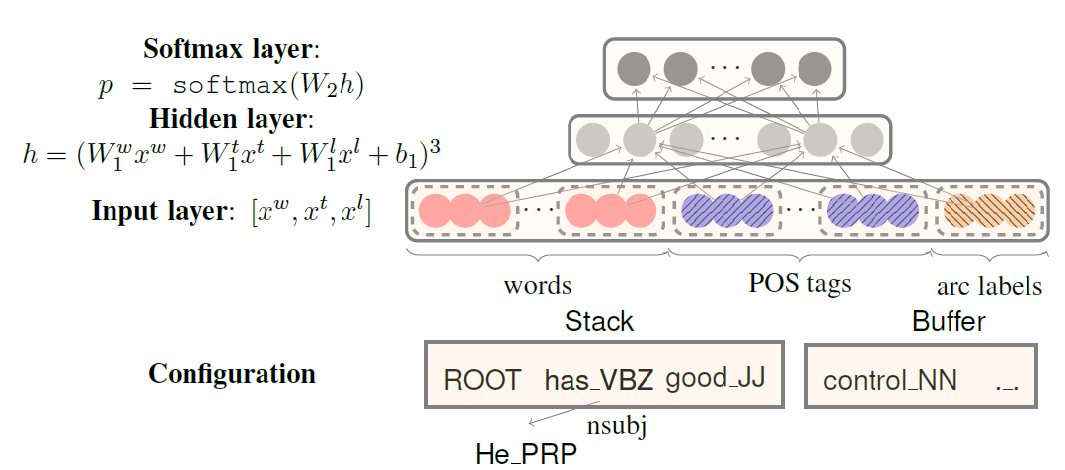
\includegraphics[scale = 0.5]{NNchenmanning.png}
    \centering
    \caption{Neural Network architecture}
    \label{fig:NNchenmanning}
\end{figure*}

A greedy decoding is performed for parsing. At every step, word, its POS and label embeddings are extracted from the current configuration and like all the transition based parsers, the transition with the highest score is selected. This work is shown for the projective case only. For the selected sentences in PTB and CTB, this parser works better than MaltParser and MST in terms of parsing time and accuracy. 
\cite{weiss2015structured} followed a similar approach but instead of one hidden layer, they added two which slightly improved the parser accuracy. Their work differs from Chen and Manning's by the use of semi-supervised structured learning which is implemented for the training. To learn the final layer of the model, they make use of structured perceptron. They also introduce unlabeled data by using word embeddings. This work was further extended for multilingual cases~\cite{alberti2015improved}. The difference is in the use of set or bag of features which are embedded into the same embedding space. 
Chen and Manning's neural network architecture for parsing was further modified by 
\cite{zhou2015neural} using beam search for the decoding step and contrastive learning to maximize the sentence-level log likeliood. They reported 1.8\% increase in accuracy over Chen and Manning's greedy neural parser.

A graph-based neural network parser was proposed by Pei~\etal~\cite{pei2015effective} which made use of a $tanh-cubic$ activation function instead of Chen and Manning cubic activation function. The parser outperformed the baseline graph-based parsers. However, it is not clear if this parser outperforms the other neural network based parsers. Neural network parsers for multilingual settings are implemented by using convolutional neural networks by Zhang~\etal~\cite{zhang2016probabilistic} by using the basic architecture of Pei~\etal.

\section{Transformation Based Error Driven Learning}~\label{sec:TBL}

\begin{figure}[t!]
\centering
    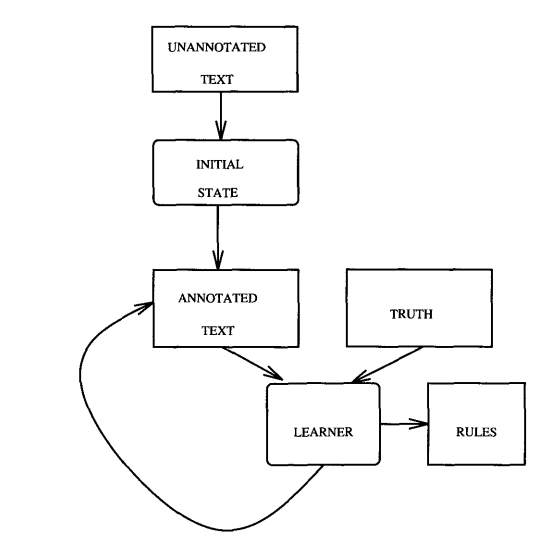
\includegraphics[scale=0.8]{tbl-brill.png}
\caption{Transformation Based Error Driven Parsing}~\citep{brill1992simple}
\label{tbl:brill}
\end{figure}

The underlying idea of transformation based error driven learning (TBL) is shown in figure~\ref{tbl:brill}. Transformation based error driven learning (TBL) was originally developed for POS tagging \cite{brill1992simple,Brill:1995:TEL:218355.218367}. The idea is straightforward, yet effective. We have a set of unannotated text. We run it through an ``initial" state system, which is dependent on the task. E.g., in Brill's case, it was a stochastic $n$-gram tagger. This produces an initial annotation, albeit not a good/accurate one. However, the errors in the initial annotation can be continually improved by comparing it to the ground truth or the gold standard. Each such annotation passes through multiple iterations of error correction, until there is no more improvement in terms of reduction of errors. In repeating this process, the TBL process accumulates a set of rules, which is the final output. This is the training phase, which essentially learns from the errors and creates a set of rules. Now, that we have learned these rules, we can apply it to another corpus. 

As described in the previous paragraph, the method works with two versions of the training data: the gold standard and (an initially unannotated) working copy that simulates the learning process and records the errors. The unannotated version of the training data is tagged by a simple part of speech tagger\footnote{This could be any simple part of speech tagger, or a heuristic that labels every work with the most frequent POS tag}, to create the initial state of the working copy of the text.  The goal is to bridge the difference between the gold standard text and the working copy by learning rules that change the incorrect POS tags to the correct ones. 
%This is done by applying a set of rule templates repeatedly and computing the objective function. 

Learning is based on rule templates, which consist of two parts: rewrite rules and triggering environment. The templates need to be determined by the researcher, based on the problem. In general, a rule template is of the form:


\textbf{Rule Template} ${(A, B): X \rightarrow Y} $

I.e., if we observe conditions $A$ and $B$ (triggering environment), we change the output variable (POS tags, for Brill and dependency labels, for us) 
from $X$ to $Y$ (rewrite rule). Note that X can remain unspecified, then the rule is applied independent of the current variable (label or POS tag).

The following is an example of a rule template for POS tagging: Change the POS tag of the current word from X to Y if the previous word is tagged as Z, where X, Y, and Z are variables that need to be instantiated during learning. 

The learner creates rule hypotheses out of those templates by identifying incorrectly tagged words in the working copy and instantiating the template variables.
For example, one possible rule hypothesis could be the following: Change the POS tag of the word ``impact'' from verb to noun if the previous word is tagged as a determiner. %One such template can instantiate multiple transformations. 
%At each stage, a list of multiple transformations are instantiated by applying these templates. 

In one pass through the system, all possible rule hypotheses are created and ranked  based on an objective function which determines for each hypothesis how many corrections occur. The rule hypothesis with the highest score is applied to the working copy and added to the final list of transformations, stored in order, during the training process. Then the process repeats, and new rule hypotheses are generated from the templates based on the remaining errors in the working copy. The process finishes when there is no more improvement in terms of reduction of errors.~\todo{more?}

\citet{brill1994rule} also use this technique for prepositional phrase attachment disambiguation. In this case, the TBL process uses a 4-tuple corpus from WSJ section of Penn Treebank. The tuples looks like: $$<V\ NP1\ P\ NP2> \rightarrow Attachment\ decision$$
$V$ is the verb, $NP1$ is the noun phrase which is the head of the verb's object, $P$ is the preposition and $NP2$ corresponds to the head of the noun phrase controlled by the preposition. One the example rule templates in this case would be - \\
Change the attachment location from $NP1$ to $V$ if $P$ is 


\citet{brill1993automatic} also used this approach to parse text by learning a ``transformational'' grammar. The algorithm repeatedly compares the bracketed structure of the syntactic tree to the gold standard structure and learns the required transformations in the process~\todo{Expand}. 



Transformation based error driven learning has also been used for information retrieval by \citet{woodley2005applying}\todo{Expand??}.





%\section{Domain Adaptation}

\section{Evaluation}

\atrcomments{Example?}~\todo{Look at hulk}

In this section I discuss the different evaluation techniques that will be used in this thesis. I report on the standard metrics for POS tagging and dependency parsing. I discuss these metrics in detail below.
%For POS tagging I mainly report accuracy, which estimates the accuracy in predicting POS tags. For dependency parsing


\subsection{POS tagging}
    \begin{itemize}
        \item Overall Accuracy: For POS tagging, I evaluate the results based on the accuracy of identifying POS tags correctly in the test set as shown in~\ref{eq:posacc}. I.e., I measure how many tags have been correctly identified in the test set.
        \begin{equation} \label{eq:posacc}
            Accuracy = \frac{Number\ of\ correctly\ identified\ tokens}{total\ number\ of\ tokens}
        \end{equation}
        \item Accuracy for Known \& Unknown tokens: For POS tagging, unknown or out of vocabulary words (OOV) pose as a challenging problem. \texttt{tnt-diff} provides an utility to measure accuracy based on number of correct predictions for known vs. unknown words. I discuss the method employed by TnT to determine the POS tags for unknown words in section \atrcomments{TBD}. I.e., we can determine the accuracy on known and OOV words separately. Since performance on OOV words is an essential determining factor, I use this metric to further analyze the results from domain experts in greater detail. This is a bigger challenge in a domain adaptation situation since there are domain specific words for each domain, which tend to get misclassified in a heterogeneous dataset.
    \end{itemize}
\subsection{Dependency Parsing}
    \begin{itemize}
        \item Labeled Attachment Scores (LAS): For evaluating the results of dependency parsing experiments in this chapter, I report LAS\footnote{I report micro-averaged LAS. Micro-averaged LAS is reported on words as opposed to macro-averaged LAS, which considers sentences as the grain.}.  As \ref{eq:las} shows, LAS estimates the number of words with correctly predicted head and label.
        \begin{equation} \label{eq:las}
            LAS = \frac{number\ of\ words\ with\ correct\ head\ and\ label}{total\ words}
        \end{equation}
        
        \item Unlabeled Attachment Scores (UAS): UAS, as the name suggests, evaluates based on correctly predicted head. 
        \begin{equation} \label{eq:uas}
            UAS = \frac{number\ of\ words\ with\ correct\ head}{total\ words}
        \end{equation}
        
        \item Exact Match (EM): This metric determines how many sentences are parsed accurately by the parser.
        
    \end{itemize}


\section{Corpora}

In this \atrcomments{section}, I elaborate on the corpora I used for the experiments conducted on domain adaptation for POS tagging and dependency parsing. I use three main corpora as a representative of their domains. I discuss these in detail in the next sections. In addition to classical domain adaptation, the goal is also to achieve a more generic form of domain adaptation, i.e., to evaluate if my system can detect domains in a heterogeneous or mixed dataset (see \atrcomments{chapter x}). Thus, I create an artificial corpus from the corpora, which contains equal representation of two domains. Although all the corpora used in this thesis are annotated in the PTB style, each has a distinctive syntactic style, which ... ~\todo{dont know how to finish this sentence}.

%Since the goal is domain adaptation, the corpora used for the experiments need to be reasonably diverse. 
  
\subsection{Wall Street Journal section of Penn Treebank (WSJ)}

~\todo{check!!}
\footnote{https://catalog.ldc.upenn.edu/LDC2000T43}
This is the Wall Street Journal section~\citep{Marcus:1994:PTA:1075812.1075835} of the Penn Treebank~\citep{santorini:90}. \textcolor{red}{This corpus contains annotated newspaper articles from WSJ from 1987 - 1989. The corpus is annotated for POS tags and parsed in PTB bracketed style. The dependency trees are then derived using the Penn Converter Tool~\citep{johansson2007a} and the inconsistencies are addressed manually}. I use this corpus as a representative of the newspaper domains. There are various different kinds of news articles from financial news, theater critique, weather, sports, politics, etc. Thus, in addition to contributing as a main domain, we can also exploit the corpus for micro-genres or more fine-grained domains. The sentences in WSJ are reasonably longer with an average length of 24 words. I use the standard split for parsing, which is, 02-21 for training, 22 for test and 23 for validation. Some of the example sentences from WSJ are as given below.  ~\todo{EXAMPLES}
\begin{itemize}
    \item In an Oct. 19 review of " The Misanthrope " at Chicago 's Goodman Theatre ( " Revitalized Classics Take the Stage in Windy City , " Leisure & Arts ) , the role of Celimene , played by Kim Cattrall , was mistakenly attributed to Christina Haag .
    \item Japanese culture vs. American culture is irrelevant .
    \item Las Vegas promises , or threatens , to become a giant carnival , with rooms to be had for \$ 45 a day or less , for visitors uninspired solely by gambling  .
    \item To avoid default , lawmakers must pass legislation raising the limit to \$ 3.12 trillion from \$ 2.80 trillion by next Wednesday , according to the Treasury .
     
\end{itemize}

\subsection{GENIA Corpus}

The GENIA Corpus~\citep{tateisi:tsujii:04} comprises of biomedical abstracts from Medline, and it is annotated on different linguistic levels, including POS tags, syntax, coreference, and events, among others. I use GENIA 1.0 trees~\cite{Ohta:2002:GCA:1289189.1289260} created in the Penn Treebank format\footnote{http://nlp.stanford.edu/~mcclosky/biomedical.html}. The treebank is converted to dependencies using pennconverter~\cite{johansson2007a}. The tagset used in GENIA is based on the Penn Treebank tagset, but it uses the tags for proper names and symbols only in very restricted contexts. This treebank serves as a representative of biomedical domain for my experiments. Clearly, this is very distinct from WSJ in terms of the nature of the content. Some of the sentences from the corpus are shown below.~\todo{EXAMPLES}
\begin{itemize}
    \item AP-1 is an integral component of the nuclear factor of activated T cells ( NFAT ) transcriptional complex , which is required for interleukin 2 gene expression in T cells .
    \item The data further indicate that the IL-7R alpha chains are directly involved in the activation of JAKs and STATs and have a major role in proliferative signaling in precursor B cells .
    \item Gel mobility shift assays and DNase I footprinting demonstrated that GM3 formed a sequence-specific collinear triplex with its double-stranded DNA target .
    \item Generation of CD1+RelB+ dendritic cells and tartrate-resistant acid phosphatase-positive osteoclast-like multinucleated giant cells from human monocytes . 
\end{itemize}

\subsection{CReST Corpus}

The CReST corpus~\citep{eberhard2010indiana} constitutes of natural language dialogues between two individuals performing a ``cooperative, remote, search task" (CReST). This is a multimodal corpus which is annotated for speech signals and their corresponding transcriptions. The transcribed text is annotated in PTB format for constituent trees. These constituent trees are converted to dependency trees using Penn Converter~\citep{johansson2007a}. Since this is transcribed from spoken dialogues, the average length of sentence is 7. In terms of linguistic factors, CReST has a subset of WSJ's dependency labels with 10 new labels added. A few examples of the CReST corpus are given below:
\todo{EXAMPLES}

\begin{itemize}
    \item um to the right like right at the edge is
    \item it's like as soon - like if I were to close the door it's right next to like the  bottom of the floor like where the door closes
    \item and at the other end of that little hallway
    \item the - the - okay so you know where the cardboard box is where I told you ? 
\end{itemize}
% \begin{table}[t]
% \centering
% \begin{tabular}{|l|} \hline
% um to the right like right at the edge is \\ \hline
% it's like as soon - like if I were to close the door it's right next to like the  bottom of the \\ floor like where the door closes \\ \hline
% \end{tabular}
% \caption{My caption}
% \label{my-label}
% \end{table}

I use CReST as a representative target domain in my experiments. The CReST corpus consists of 23 dialogues that were manually annotated for dependencies. I randomly select 19 dialogues as my training data for the TBL algorithm and the rest as test. Since the system needs to learn rule hypotheses from incorrect predictions of the source domain parser, I can safely ignore sentences that were parsed completely correctly\footnote{Details about the split are discussed in Chapter TBL \atrcomments{TBD}}. For the test data, I use all the sentences from the designated dialogues (with correct and incorrect dependency label predictions). 
Table~\ref{tab:sentdiv} shows the division of sentences for training and test.

\begin{table}[t]
\centering
\begin{tabular}{l|l|c|c}
& \multirow{2}{*}{\# Dialogues} & \multicolumn{2}{c}{\# Sentences} \\ \cline{3-4}
 &  & \multicolumn{1}{l|}{with errors} & \multicolumn{1}{l}{without errors} \\ \hline
Training Set & \multicolumn{1}{|c|}{19} & 4384 & 459 \\
Test Set & \multicolumn{1}{|c|}{4} & 831 & 85 \\ \hline
\end{tabular}
\caption{Target domain training and test set for TBL}
\label{tab:sentdiv}
\end{table}

\subsection{WSJ-GENIA mixed corpus (WSJ+GENIA)} ~\label{sec:wsjgeniamixedcorpus}

Since my objective is to identify domains from a heterogeneous dataset and then adapt POS taggers and dependency parsers to the corresponding domain, I need a dataset which contains sentences from different domains. In order to test my hypothesis, I create an artificial corpus by incorporating data from WSJ as well as the GENIA corpus in equal measure. 

\begin{table}[t]
\centering
\begin{tabular}{l|c|c}
      & Training Set & Test Set   \\ \hline
WSJ   & 17~181  & 850        \\
GENIA & 17~181  & 850        \\ \hline
Total & 34~362  & 1~700 \\ \hline
\end{tabular}
\caption{Overview of the mixed dataset (WSJ+GENIA)}
\label{tab:mixeddata}
\end{table}

I randomly select 17~181 sentences from section 02-21 of WSJ corpus as training data and similarly select 850 sentences from section 22 for test. Then, I add equal amount of sentences from GENIA to create a heterogeneous balanced corpus. 


% I use the script \texttt{tnt-diff} that is part of TnT to evaluate the POS tagging results  and the CoNLL shared task evaluation script\footnote{http://ilk.uvt.nl/conll/software/eval.pl} for evaluating the parsing results. I report the following evaluation metrics for evaluation:

\section{Summary}



%%%%%%%%%%%%%%%%
% Chapter 3 - Domain Adaptation
%%%%%%%%%%%%%%%%

\chapter{Domain Adaptation}
\todo[inline]{domain adaptation lit review+research questions}

Domain adaptation is a well studied problem in machine learning and natural language processing. Usually, there is a plenty of labeled data available for one domain (also known as the source domain) but nearly not enough or in some cases, none available from a different domain (also known as target). The challenge in that case, is to apply well performing systems from source domain and adapt it the target domain. In most problems, this results in a drop in performance, sometimes severe. The same holds true for POS tagging and dependency parsing. These systems perform well when trained and tested on datasets that are predominantly in the same text domain. However, there is a considerable decrease in accuracy if the domains under consideration, are markedly different. It is a well-studied problem for POS tagging and dependency parsing (more so for dependency parsing) but the improvement proposed by these systems have been negligible at best. This is mainly due to unavailability of annotated data from target domain. \cite{daume:07} notes that this problem is ``frustratingly easy'' when some annotated data  is available from the target domain  and ``frustratingly hard'' if no such target data is available~\citep{dredze:blitzer:ea:07}. 

%Previous work in this area have largely focused on the classic domain adaptation problem. The closest comparison to my approach is the one by \cite{plank2011effective}. However, the problem they address is creating a specialized training set for every document they need to parse. They pick sentences from the training set which are most similar to test set. Topic distribution is thus used as features for similarity metrics. My approach is a more general, because I create more general domain training ``experts". My approach also draws parallel with the work on ``multiple source parse adaptation" by \cite{mcclosky2010automatic}. In this approach the parser is trained on multiple domains and learned the statistics as well as  domain differences which affect the parser accuracy. This is similar to my approach as I create experts based on topics , and each expert learns the specifics of the particular topic with which it is associated.

%%%%%%%%%%%%%%%%
% Chapter 4 - Corpus
%%%%%%%%%%%%%%%%

%% \chapter{Corpora}

% In this chapter, I elaborate on the corpora I used for the experiments conducted on domain adaptation for POS tagging and dependency parsing. I use three main corpora as a representative of their domains. I discuss this in detail in the next sections. In addition to classical domain adaptation, the goal is also to achieve a more generic form of domain adaptation, i.e., to evaluate if my system can detect domains in a heterogeneous or mixed dataset. Thus, I create an artificial corpus from the corpora, which contains equal representation of two domains. Although all the corpora used in this thesis are annotated in the PTB style, each has a distinctive syntactic style, which ... ~\todo{dont know how to finish this sentence}.

% %Since the goal is domain adaptation, the corpora used for the experiments need to be reasonably diverse. 
  
% \section{Wall Street Journal section of Penn Treebank (WSJ)}

% ~\todo{check!!}
% \footnote{https://catalog.ldc.upenn.edu/LDC2000T43}
% This is the Wall Street Journal section~\citep{Marcus:1994:PTA:1075812.1075835} of the Penn Treebank~\citep{santorini:90}. \textcolor{red}{This corpus contains annotated newspaper articles from WSJ from 1987 - 1989. The corpus is annotated for POS tags and parsed in PTB bracketed style. The dependency trees are then derived using the Penn Converter Tool~\citep{johansson2007a} and the inconsistencies are addressed manually}. I use this corpus as a representative of the newspaper domains. There are various different kinds of news articles from financial news, theater critique, weather, sports, politics, etc. Thus, in addition to contributing as a main domain, we can also exploit the corpus for micro-genres or more fine-grained domains. The sentences in WSJ are reasonably longer with an average length of 24 words. I use the standard split for parsing, which is, 02-21 for training, 22 for test and 23 for validation. Some of the example sentences from WSJ are as given below.  ~\todo{EXAMPLES}
% \begin{itemize}
%     \item In an Oct. 19 review of " The Misanthrope " at Chicago 's Goodman Theatre ( " Revitalized Classics Take the Stage in Windy City , " Leisure & Arts ) , the role of Celimene , played by Kim Cattrall , was mistakenly attributed to Christina Haag .
%     \item Japanese culture vs. American culture is irrelevant .
%     \item Las Vegas promises , or threatens , to become a giant carnival , with rooms to be had for \$ 45 a day or less , for visitors uninspired solely by gambling  .
%     \item To avoid default , lawmakers must pass legislation raising the limit to \$ 3.12 trillion from \$ 2.80 trillion by next Wednesday , according to the Treasury .
     
% \end{itemize}

% \section{GENIA Corpus}

% The GENIA Corpus~\citep{tateisi:tsujii:04} comprises of biomedical abstracts from Medline, and it is annotated on different linguistic levels, including POS tags, syntax, coreference, and events, among others. I use GENIA 1.0 trees~\cite{Ohta:2002:GCA:1289189.1289260} created in the Penn Treebank format\footnote{http://nlp.stanford.edu/~mcclosky/biomedical.html}. The treebank is converted to dependencies using pennconverter~\cite{johansson2007a}. The tagset used in GENIA is based on the Penn Treebank tagset, but it uses the tags for proper names and symbols only in very restricted contexts. This treebank serves as a representative of biomedical domain for my experiments. Clearly, this is very distinct from WSJ in terms of the nature of the content. Some of the sentences from the corpus are shown below.~\todo{EXAMPLES}
% \begin{itemize}
%     \item AP-1 is an integral component of the nuclear factor of activated T cells ( NFAT ) transcriptional complex , which is required for interleukin 2 gene expression in T cells .
%     \item The data further indicate that the IL-7R alpha chains are directly involved in the activation of JAKs and STATs and have a major role in proliferative signaling in precursor B cells .
%     \item Gel mobility shift assays and DNase I footprinting demonstrated that GM3 formed a sequence-specific collinear triplex with its double-stranded DNA target .
%     \item Generation of CD1+RelB+ dendritic cells and tartrate-resistant acid phosphatase-positive osteoclast-like multinucleated giant cells from human monocytes . 
% \end{itemize}

% \section{CReST Corpus}

% The CReST corpus~\citep{eberhard2010indiana} constitutes of natural language dialogues between two individuals performing a ``cooperative, remote, search task" (CReST). This is a multimodal corpus which is annotated for speech signals and their corresponding transcriptions. The transcribed text is annotated in PTB format for constituent trees. These constituent trees are converted to dependency trees using Penn Converter~\citep{johansson2007a}. Since this is transcribed from spoken dialogues, the average length of sentence is 7. In terms of linguistic factors, CReST has a subset of WSJ's dependency labels with 10 new labels added. A few examples of the CReST corpus are given below:
% \todo{EXAMPLES}

% \begin{itemize}
%     \item um to the right like right at the edge is
%     \item it's like as soon - like if I were to close the door it's right next to like the  bottom of the floor like where the door closes
%     \item and at the other end of that little hallway
%     \item the - the - okay so you know where the cardboard box is where I told you ? 
% \end{itemize}
% % \begin{table}[t]
% % \centering
% % \begin{tabular}{|l|} \hline
% % um to the right like right at the edge is \\ \hline
% % it's like as soon - like if I were to close the door it's right next to like the  bottom of the \\ floor like where the door closes \\ \hline
% % \end{tabular}
% % \caption{My caption}
% % \label{my-label}
% % \end{table}

% I use CReST as a representative target domain in my experiments. The CReST corpus consists of 23 dialogues that were manually annotated for dependencies. I randomly select 19 dialogues as my training data for the TBL algorithm and the rest as test. Since the system needs to learn rule hypotheses from incorrect predictions of the source domain parser, I can safely ignore sentences that were parsed completely correctly\footnote{Details about the split are discussed in Chapter TBL \atrcomments{TBD}}. For the test data, I use all the sentences from the designated dialogues (with correct and incorrect dependency label predictions). 
% Table~\ref{tab:sentdiv} shows the division of sentences for training and test.

% \begin{table}[t]
% \centering
% \begin{tabular}{l|l|c|c}
% & \multirow{2}{*}{\# Dialogues} & \multicolumn{2}{c}{\# Sentences} \\ \cline{3-4}
%  &  & \multicolumn{1}{l|}{with errors} & \multicolumn{1}{l}{without errors} \\ \hline
% Training Set & \multicolumn{1}{|c|}{19} & 4384 & 459 \\
% Test Set & \multicolumn{1}{|c|}{4} & 831 & 85 \\ \hline
% \end{tabular}
% \caption{Target domain training and test set for TBL}
% \label{tab:sentdiv}
% \end{table}

% \section{WSJ-GENIA mixed corpus (WSJ+GENIA)} ~\label{sec:wsjgeniamixedcorpus}

% Since my objective is to identify domains from a heterogeneous dataset and then adapt POS taggers and dependency parsers to the corresponding domain, I need a dataset which contains sentences from different domains. In order to test my hypothesis, I create an artificial corpus by incorporating data from WSJ as well as the GENIA corpus in equal measure. 

% \begin{table}[t]
% \centering
% \begin{tabular}{l|c|c}
%       & Training Set & Test Set   \\ \hline
% WSJ   & 17~181  & 850        \\
% GENIA & 17~181  & 850        \\ \hline
% Total & 34~362  & 1~700 \\ \hline
% \end{tabular}
% \caption{Overview of the mixed dataset (WSJ+GENIA)}
% \label{tab:mixeddata}
% \end{table}

% I randomly select 17~181 sentences from section 02-21 of WSJ corpus as training data and similarly select 850 sentences from section 22 for test. Then, I add equal amount of sentences from GENIA to create a heterogeneous balanced corpus. 

% \section{Summary}

% \atrcomments{TBD}

% % \subsection{Data Sets}

% % For our experiments, we use the Wall Street Journal (WSJ) section of
% % the Penn Treebank \cite{marcus:kim:ea:94} and the GENIA Corpus \cite{tateisi:tsujii:04}. Both corpora use the Penn
% % Treebank POS tagset \cite{santorini:90} with minor differences: The tagset used in
% % GENIA is based on the Penn Treebank tagset, but it uses the tags for
% % proper names and symbols only in very restricted contexts. 

% % For the WSJ corpus, we extract the POS annotation from the
% % syntactically annotated corpus. The GENIA Corpus comprises biomedical
% % abstracts from Medline, and it is annotated on different
% % linguistic levels, including POS tags, syntax, coreference, and
% % events, among others. We use GENIA 1.0 trees~\cite{Ohta:2002:GCA:1289189.1289260} created in the Penn Treebank format\footnote{http://nlp.stanford.edu/~mcclosky/biomedical.html}. Both treebanks were converted to dependencies using pennconverter~\cite{johansson2007a}.

% % For our experiments, we need a balanced data set, both for the training and
% % the test set. Since GENIA is rather small and since there is no standard data split for GENIA, we decided to extract the last 850 sentences for the test set. The remaining 17~181 sentences are used for training. For WSJ, we chose the same number of sentences for both training and the test set, the training sentences are selected randomly from sections 02-21 and the test sentences from section 22.\ignore{SK: is that correct?} 




% % \section{Corpus}
% % \todo[inline]{EACL+ICON}

% % \subsection{Wall Street Journal section of Penn Treebank (WSJ)}
% % WSJ~\cite{Marcus:1994:PTA:1075812.1075835} - This is the Wall Street Journal section of the Penn Treebank~\cite{santorini:90}. This dataset consists of newspaper articles/reports from the financial domain as well as reports on politics, weather, etc. This is the representative of the newspaper domain.

% % \subsection{Data Sets}


% % For our experiments, we use the Wall Street Journal (WSJ) section of the Penn Treebank \cite{marcus:kim:ea:94} and the GENIA Corpus (version 3.02) \cite{tateisi:tsujii:04}. Both corpora use the Penn Treebank POS tagset \cite{santorini:90} with minor differences.%, as described in section \ref{sec:q1}.

% % For the WSJ corpus, we extract the POS annotation from the syntactically annotated corpus. The GENIA Corpus comprises biomedical abstracts from Medline, and it is annotated on different linguistic levels, including POS tags, syntax, coreference, and events, among others. We use the POS tagged version. For WSJ, we use the standard data split for parsing:  using sections 02-21 as training data and section 22 as our test set. We reserve section 23 for future parsing expert experiments.

% % \subsection{Data Sets}
% % In our current work, we focus on two domains: financial news articles and dialogues in a collaborative task.
% % We use the Wall Street Journal \cite{Marcus:1994:PTA:1075812.1075835} and the CReST corpus~\cite{eberhard2010indiana} as representative corpora for these two domains. For both corpora, we use teh dependency version: CReST was originally annotated in constituents and dependencies, the Penn Treebank was automatically converted to dependencies using \textit{pennconverter} \cite{johansson2007a}. %Wall Street Journal consists of financial articles, news, etc. CReST corpus, on the other hand, comprises of dialogues recorded during a collaborative task.%natural language dialogues between two people, who carry out a certain task with the help of each other. 
% % %%SK check numbers? - x

% % These corpora are very dissimilar in nature. On an average, the length of the sentences for WSJ is 24 and 7 for CReST. In terms of linguistic factors, CReST has a subset of WSJ's dependency labels with 10 new labels added. %and 
% % %%SK why do we care about POS tags? should that be dep labels? - atr: because I was thinking this might also show how different the corpora are, but its not needed.
% % %has 14 different part of speech tags than WSJ. 
% % Example sentences from each corpora are shown in table~\ref{tab:samplesentences}. We use WSJ as the source domain and CReST as the target domain.  %We create a parsing model using the MATE parser~\cite{bohnet:2010:PAPERS,bohnet2010very}. We then parse sentences from CReST using this model. %Since the source domain (WSJ) and the target domain (CReST) have differences in dependency label annotation, this introduces some errors in the resulting parse. 

% % \begin{table}[!t]
% % \centering
% % \begin{tabular}{l|l}
% % \hline
% % WSJ   & \begin{tabular}[c]{@{}l@{}}
% % In an Oct. 19 review of " The Misanthrope " at Chicago 's Goodman Theatre \\ ( " Revitalized Classics Take the Stage in Windy City , " Leisure \& Arts ) , \\ the role of Celimene , played by Kim Cattrall , was mistakenly attributed \\ to Christina Haag .\end{tabular} \\ \hline
% % CReST & \begin{tabular}[c]{@{}l@{}}
% % it's like as soon - like if I were to close the door it's right next to like the \\ bottom of the floor like where the door closes 
% % \end{tabular} \\ \hline
% % %so I went through some - I went through the second room right? \\ \hline    
% % %can I tell you where that is?   
% % \end{tabular}
% % \caption{Sample sentences from Wall Street Journal (WSJ) \& CReST corpus}
% % \label{tab:samplesentences}
% % \end{table}



% % \paragraph{Target Domain}
% % The CReST corpus consists of 23 dialogues that were manually annotated for dependencies. We randomly select 19 dialogues as our training data for the TBL algorithm and the rest as test. 
% % Since the system needs to learn rule hypotheses from  incorrect predictions of the source domain parser, 
% % we can safely ignore sentences that were parsed completely correctly. For the test data, we use all the sentences from the designated dialogues (with correct and incorrect dependency label predictions). 
% % %As a part the training part of Transformation Based Error Driven Learning (TBL), the system needs to learn rule hypotheses from the incorrect dependency label prediction, we work on the sentences which show errors in dependency labels. 
% % Table~\ref{tab:sentdiv} shows the division of sentences for training and test.

% % \begin{table}[t]
% % \centering
% % \begin{tabular}{l|l|c|c}
% % & \multirow{2}{*}{\# Dialogues} & \multicolumn{2}{c}{\# Sentences} \\ \cline{3-4}
% %  &  & \multicolumn{1}{l|}{with errors} & \multicolumn{1}{l}{without errors} \\ \hline
% % Training Set & \multicolumn{1}{|c|}{19} & 4384 & 459 \\
% % Test Set & \multicolumn{1}{|c|}{4} & 831 & 85 \\ \hline
% % \end{tabular}
% % \caption{Target domain training and test set for TBL}
% % \label{tab:sentdiv}
% % \end{table}




%%%%%%%%%%%%%%%%
% Chapter 5 - Experts
%%%%%%%%%%%%%%%%

\chapter{Domain Experts via Topic Modeling}


\section{Introduction}

Domain adaptation is a well studied problem in machine learning and natural language processing. Usually, there is a plenty of labeled data available for one domain (also known as the source domain) but nearly not enough or in some cases, none available from a different domain (also known as target). The challenge in that case, is to apply well performing systems from source domain and adapt it the target domain. In most problems, this results in a drop in performance, sometimes severe. The same holds true for POS tagging and dependency parsing. These systems perform well when trained and tested on datasets that are predominantly in the same text domain. However, there is a considerable decrease in accuracy if the domains under consideration, are markedly different. It is a well-studied problem for POS tagging and dependency parsing (more so for dependency parsing) but the improvement proposed by these systems have been negligible at best. This is mainly due to unavailability of annotated data from target domain. \cite{daume:07} notes that this problem is ``frustratingly easy'' when some annotated data  is available from the target domain  and ``frustratingly hard'' if no such target data is available~\citep{dredze:blitzer:ea:07}. 

In this chapter, I address a problem which is analogous to this classic domain adaptation problem since the aim is to improve (morpho-)syntactic analysis for different domains, but more generic in nature. In order to simulate a more realistic scenario, I assume that the  dataset on which the taggers and the parsers is trained on, does not come from a single domain but may contain a mix of different domains. The same is true for the sentence that is parsed (or tagged) using the model trained on this dataset. I.e., the test sentence could potentially come from any of the domains. Thus, in my case, the problem is two fold - identify domains automatically in the training dataset and then suitably adapt the method to parse sentences more accurately. There is no manual work involved. 

Previous work in this area have largely focused on the classic domain adaptation problem. The closest comparison to my approach is the one by \cite{plank2011effective}. However, the problem they address is creating a specialized training set for every document they need to parse. They pick sentences from the training set which are most similar to test set. Topic distribution is thus used as features for similarity metrics. My approach is a more general, because I create more general domain training ``experts". My approach also draws parallel with the work on ``multiple source parse adaptation" by \cite{mcclosky2010automatic}. In this approach the parser is trained on multiple domains and learned the statistics as well as  domain differences which affect the parser accuracy. This is similar to my approach as I create experts based on topics , and each expert learns the specifics of the particular topic with which it is associated.

In this chapter, I describe my method on improving POS tagging and dependency parsing for such heterogeneous datasets from a variety of different genres by creating experts for automatically detected topics. In this case, the datasets consist of newspaper reports on the one hand and biomedical extracts on the other. I assume that the domains have an equal participation in the dataset. I use Latent Dirichlet Allocation (LDA) to determine the topic of a sentence. LDA displays the latent topic structure in a document. In this case, a document to be clustered consists of a single sentence. I then assign each sentence to the most likely topic, for both training and test sentences. I train an expert for each topic and then use this expert to POS tag and parse the test sentences belonging to this topic. I assume that the topics detected by the topic modeler do not only pertain to lexical differences, which can be beneficial for the POS tagger and the parser, but also to syntactic phenomena. Thus, one topic may focus on ``incomplete" sentences, such as headlines in a newspaper.

The rest of the chapter is structured in the following way: \atrcomments{TBD after completion}


\section{Research Questions}\label{sec:quest}

The goal is to create POS tagging and parsing experts for heterogeneous datasets which consist of  sentences from different genres. For example, the dataset might be a mixture of newspaper articles, blogs, financial reports, research papers and even specialized texts such as biomedical research papers and law texts. I create experts such that each expert would learn specific information about its own genre. I determine these experts by performing topic modeling on sentences and then train an expert on the sentences of the topic. I group sentences based on their most probable topic. To test the hypothesis that topic modeling can serve to group sentences into topics, I create a mixed dataset from the financial domain (using the Penn Treebank \cite{marcus:kim:ea:94}) and from the biomedical domain (using the GENIA Corpus \cite{tateisi:tsujii:04}) such that the new handcrafted corpus consists of sentences from both domains in equal measure. Consequently, there is a clear difference in the genres in the corpus, and I have gold standard topic information.

In this chapter, I investigate the possibility of creating genre experts, given a heterogeneous dataset. Thus, I perform topic modeling on training and test data simultaneously: I assign a test sentence to the topic with the highest probability. This means that I currently simplify the problem of assigning new sentences to topics. In the next chapter, I assign new sentences to topics based their similarity to sentences in the topics created during training, following the work by \newcite{plank2011effective}. 

To summarize, I present the results on the following research questions in this chapter.

\subsection*{Question 1: Can topic modeling successfully identify genres in a dataset?} \label{q1}

\atrcomments{need to remove WSJ ones for now}

In this question, I determine whether the data splits obtained from the topic modeler are meaningful for creating domain experts. I.e., I investigate whether an unsupervised topic modeler can detect topics in a heterogeneous corpus. I use an artificially created heterogeneous corpus containing sentences from the Wall Street Journal (WSJ) section of the Penn Treebank \citep{marcus:kim:ea:94} and  from the GENIA Corpus \citep{tateisi:tsujii:04} and take their original corpus as the gold standard topic. I assume that a good split into the known topics, financial news and biomedical abstracts, will also improve POS tagging and parsing accuracy. 
If I assume two topics, we should be able to see a clear distinction between WSJ and GENIA sentences. I.e., for each topic, we should have a clear correspondence of its sentences to either WSJ or GENIA. I thus calculate the percentage of sentences in a given topic that belong to GENIA and expect that one topic should have a high percentage and the other one a low percentage. I also experiment with a larger number of topics, to see if I can profit from a finer grained topic definition. However, this advantage will be offset by a smaller training set since we split into more sets. 

%\atrcomments{Needs parsing experiments/need to check in the results sheet if this is there}

%\atrcomments{REMOVE} The finer grained split could also potentially identify micro-genres within a genre. I.e., the primary assumption is that - there are two very different genres and the topic modeler should be able to identify this distinction. In my case, WSJ and GENIA are representative of corpora from two very different domains - newspaper and biomedical texts. However, often the distinction between genres could be subtle. In that case, it is imperative to check if topic modeler could also identify micro-genres, in addition to the broader classification. To investigate this, I exclusively use the WSJ data set. The hypothesis is that the WSJ corpus contains different newspaper sections, which may use different styles. Since there is no information available from the Penn Treebank about those section, I cannot evaluate how well the topic modeler splits the sentences into topics, but I can evaluate whether the POS tagging/\atrcomments{parsing} experts are successful in adapting to those micro-genres.

\subsection*{Question 2: How do we cluster sentences into experts?}

In the previous question, I mentioned that having a finer grained split, i.e., larger number of topics could result in severe data sparseness. This is assuming that we treat topics as hard clusters, i.e., every sentence belongs to the topic with the highest probability. However, this is a simplification since a sentence can represent different topics to different degrees. This is especially true in case of identifying micro-genres or larger number of topics, in general. Thus, a potential solution is to investigate whether we can utilize the soft clustering information directly and add every sentence to every domain expert, weighted based on the degree to which it represents the topic of this expert. This not only allows us to model topics in more detail, it can also help combating data sparsity since every sentence contributes to every expert. The risk is that I ``diffuse'' the expert knowledge too much by adding all sentences even if they are weighted. 

\subsection*{Question 3: Does POS Tagging Benefit from Using Topics?}

In this question, I examine whether the performance of POS tagging improves if we create experts based on the topics detected by the topic modeler. 
In order to investigate this question, I generate a two-topic corpus by combining data from the Wall Street Journal (WSJ) section of the Penn Treebank \cite{marcus:kim:ea:94} and from the GENIA corpus \cite{tateisi:tsujii:04}. The WSJ covers financial news while GENIA uses Medline abstracts as its textual basis. As a consequence, I have sentences from two different genres, but also slight variations in the POS tagsets. The tagset used in GENIA is based on the Penn Treebank tagset, but it uses the tags for proper names and symbols only in very restricted contexts. This setup allows me to test whether the topic modeler is able to distinguish the two genres, and whether POS tagging experts can profit from this separation. I use the topics created for the previous sections and train a POS tagging expert on the training part of each topic. I then use the expert to tag the test sentences from this topic. In this setting, we can see  if the experts can effectively handle the data sparseness caused by dividing the training set into multiple experts. I experiment with one setting in which I use topic modeling as hard clustering, i.e., I assign each sentence to the topic for which the topic modeler gave the highest probability. I also experiment with soft clustering, in which I add each sentence to all topics, weighted by its probability distribution.

\subsection*{Question 4: Does Dependency Parsing Benefit from the Topics?}

Here, I investigate the effects of using topic modeling experts for dependency parsing. I first use gold POS tags in order to abstract away from POS tagging quality. In a second step, I investigate the interaction between POS tagging and parsing experts. I.e., I am interested in whether dependency parsing can profit from using the POS tags that were determined by the POS tagging experts. This helps in determining whether integrating POS information given by the POS experts can improve dependency parsing or whether there is no interaction between the two levels.

\subsection*{Question 5: What do the Experts Learn?}

In this question, I take a closer look at the results from the previous question to learn where the improvements by the experts (POS tagging \& parsing) are come from. I investigate on certain known issues for both POS tagging and dependency parsing in domain adaptation situation and in general, to ascertain the source of these improvements. 

For POS tagging, out of vocabulary words are a major concern. Hence, I analyze whether all the improvements based on lower rates of out-of-vocabulary words. For example, suppose we have two experimental settings, both using the same size of the training set, but in one setting, the majority of the training set is from GENIA while in the second setting, the training set is a mix of GENIA and WSJ. It is more likely that the former will contain a wider range of biomedical vocabulary than the latter. However, it is also possible that the experts will learn different regularities, for example with regard to how the proper name tags are used in the two corpora. Thus, I look at the ratio of unknown words in the different experiments and at the error rates of known and unknown words. I additionally look at the confusion matrices.

I also analyze the parsing results in more detail to gauge the effect of using topic modeling experts. Here, I'm primarily interested in whether there are specific types of sentences or dependencies that are grouped by the topic models, so that the parsing experts focus on a specific subset of syntactic properties. Genre differences can be captured by adapting to certain syntactic phenomena. Hence, I look more closely if there is a particular type of sentence that benefit from using experts over the general case. Mislabeling of dependency is another problem, which can impact overall performance of the parser. I look at confusion matrices for dependency labels to further investigate if there is an improvement from using the experts. 

\section{Experimental Setup}\label{sec:setup}


\subsection{Data Sets}

\atrcomments{TBD}

For our experiments, we use the Wall Street Journal (WSJ) section of
the Penn Treebank \cite{marcus:kim:ea:94} and the GENIA Corpus
(version 3.02) \cite{tateisi:tsujii:04}. Both corpora use the Penn
Treebank POS tagset \cite{santorini:90} with minor differences, as
described in section \ref{sec:q1}.

For the WSJ corpus, we extract the POS annotation from the
syntactically annotated corpus. The GENIA Corpus comprises biomedical
abstracts from Medline, and it is annotated on different
linguistic levels, including POS tags, syntax, coreference, and
events, among others. We use the POS tagged version. For WSJ, we use
the standard data split for parsing:  using sections 02-21 as training data and
section 22 as our test set. We reserve section 23 for future 
parsing expert experiments.



\subsection{Topic Modeling}\label{sec:tm}

Probabilistic topic modeling is a class of algorithms which detects
the thematic structure in a large volume of documents. Topic modeling
is unsupervised, i.e., it does not require annotated
documents \cite{Blei:2012:PTM:2133806.2133826} but rather discovers similarity between documents. Latent Dirichlet
Allocation (LDA) is one of the topic modeling algorithms. It is a
generative probabilistic model that approximates the underlying hidden topical structure of a collection of texts based on the distribution of words in the documents \cite{Blei:2003:LDA:944919.944937}. I explain LDA in more detail below.

\paragraph*{LDA} 

Intuitively, Latent Dirichlet Allocation (LDA) is a method for discovering the hidden topics in a sentence. E.g., consider the following WSJ sentence. If we choose to model this in terms of LDA, we get the output shown in table~\ref{tab:2topicssent} and \ref{tab:10topicssent}.


``Though growers can't always keep the worm from the apple , they can protect themselves against the price vagaries of any one variety by diversifying -- into the recently imported Gala , a sweet New Zealand native ; the Esopus Spitzenburg , reportedly Thomas Jefferson's favorite apple ; disease-resistant kinds like the Liberty."
 
 % Please add the following required packages to  document preamble:
%\usepackage{multirow}
\begin{table*}[!htb]
\centering

\caption{2 topics distribution}
\begin{tabular}{cc}
%\multicolumn{2}{c}{2-topic probability distribution} 
\\ \hline
0 & 1 \\
95.90 & 4.10 \\ \hline
\end{tabular}
\label{tab:2topicssent}

\caption{10 topics distribution
%\\ 
}
\begin{tabular}{cccccccccc}
%\multicolumn{10}{c}{10-topic probability distribution} 
\\ \hline

0 & \multicolumn{1}{c}{1} & \multicolumn{1}{c}{2} & \multicolumn{1}{c}{3} & \multicolumn{1}{c}{4} & \multicolumn{1}{c}{5} & \multicolumn{1}{c}{6} & \multicolumn{1}{c}{7} & \multicolumn{1}{c}{8} & \multicolumn{1}{c}{9} \\
0.11 & 0.10 & 0.08 & 0.10 & 0.09 & 30.58 & 15.28 & 49.55 & 3.93 & 0.16 \\ \hline
\end{tabular}
\label{tab:10topicssent}

%\caption{2 \& 10-topic probability distribution for a WSJ corpus sentence: \\ }
%\label{tab:10t-probab}
\end{table*}

I.e., when we choose the number of topics as 2 \& 10, LDA creates a probabilistic distribution of topics in the sentence. This process of discovering topics in a document can be represented by a generative model. Each document($W$), i.e., a sentence in this case, is a mixture of topics. In other words, a sentence consists of a collection of words, i.e., $W = {w_1,w_2, ..., w_N}$. A corpus can be represented as a collection of $M$ sentences or documents, i.e., $C = {W_1, W_2, ..., W_M}$. For each sentence in a corpus, the generative steps for LDA can be given as below:
\begin{itemize}
    \item The number of words in a sentence i.e., $N$ is chosen from a Poisson distribution.
    $$N \sim Poisson(\lambda)$$
    \item The mixture of topic for a sentence is chosen according to the dirichlet distribution over a fixed set of topics.
    $$\theta \sim Dirichlet(\alpha)$$
    \item Each word ($w_i$) in sentence ($W$) can be generated as follows:
    \begin{itemize}
        \item Pick a topic according to the multinomial distribution sampled above.
        $$Z_n \sim Multinomial(\theta)$$
        \item Generate the word from the topic according to the multinomial distribution of topics. I.e., we choose a word from $p(w_n|Z_n, \beta)$, where $\beta$ represents word probabilities.
    \end{itemize}
    
    
\end{itemize}

The inference step follows the generative step, which requires calculating the posterior distribution of the hidden variables given a sentence. 
\atrcomments{to be finished ........}




\begin{figure*}[t]
    \centering
    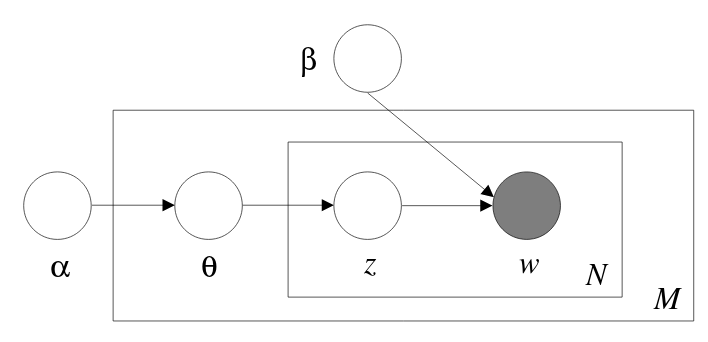
\includegraphics[width=\textwidth]{figures/LDA_plate_diagram.png}
 \caption{Graphical model for LDA~\citep{Blei:2003:LDA:944919.944937}}\label{fig:ldaplate}   
 \end{figure*}
 
 Figure~\ref{fig:ldaplate} shows the plate diagram for graphical model for LDA. Plate diagrams are standard for representing repeating entities in a graphical model for Bayesian inference. 
 
%https://www.seas.upenn.edu/~cis520/lectures/LDA.pdf
 
 



\paragraph*{LDA toolkit}

There are several  open sourced toolkits available for LDA. We use the topic modeling toolkit MALLET \cite{McCallumMALLET}.  The
topic modeler in MALLET implements Latent Dirichlet Allocation (LDA), clustering
documents into a predefined number of topics. As a result, it provides
different types of information such as:

\begin{itemize}
	\item  Topic keys:  The highest ranked words per topic with their probabilities; 
	
	\item Document topics: The topic distribution for each document (i.e., the probability that a document belongs to a given topic); and 
	
	\item Topic state: This correlates all words and topics.
	
\end{itemize}



%We can determine experts based on hard or soft clustering decisions: For question 1 and 3, the sentences are assigned to hard topics, based on the topic that has the highest probability in that sentence. I.e., if for sentence $s_x$, MALLET lists the topic $t_1$ as the topic with the highest probability, then $s_x$ is added to the data set of topic $t_1$. In other words, the data set of topic $t_1$ consists of all sentences for which MALLET showed topic $t_1$ as the most likely topic. This means that the data set sizes vary between topics. 

%For questions 2 and 3, we utilize the entire topic distribution of a sentence by weighting sentences in the training data based on their topic distribution. Since the POS tagger does not support the weighting of training examples and since we do not have access to the code of the POS tagger, we simulate weighting training sentences by adding multiple copies to the training files of the experts. Thus, for the 2-topic experiments, a sentence with 80\% probability for topic~1 will be included 80 times in the expert for topic~1 and 20 times in the expert for topic~2. We repeat these experiments, adding a sentence per every 10\%, but rounding up small percentages so that every sentence will be added to every expert at least once.  Thus, we use a more fine grained topic model to mitigate data sparseness,  but we risk adding non-typical or irrelevant sentences to experts.


\subsection{POS Tagging}
\atrcomments{More detail in the introductory chapter}

For part of speech tagging, I use the TnT (Trigrams'n'Tags) tagger \cite{brants:00.2}. TnT is based on a second order Markov Model and has an elaborate model for guessing the POS tags for unknown words. I use TnT mainly because of its speed and because it allows the manual inspection of the trained models (emission and transition frequencies).

\subsection{Overall Architecture}

\begin{figure*}[!t]
    \centering
    \includegraphics[width=\textwidth]{figures/approach.png}
 \caption{Overview of the architecture of the POS tagging and parsing experts.}\label{fig:architecture0}   
 \end{figure*}

Figure~\ref{fig:architecture0} shows the overall architecture of the system. 
I use sentences as documents. Based on the document topic information, I then group the sentences into genre topics. I collect all sentences from the training and test set, cluster them via the MALLET topic modeler, and determine for which expert(s) the sentence is relevant to. There are several ways of determining the best expert based on the probability distribution of topics in a sentence. Then, we separate the sentences for each expert into training and test sentences, based on the previously determined data splits (see above).

The experts can be determined based on hard or soft clustering decisions: For hard clustering, the sentences are assigned to hard topics, based on the topic that has the highest probability in that sentence. I.e., if for sentence $s_x$, MALLET lists the topic $t_1$ as the topic with the highest probability, then $s_x$ is added to the data set of topic $t_1$. In other words, the data set of topic $t_1$ consists of all sentences for which MALLET showed topic $t_1$ as the most likely topic. This means that the data set sizes vary between topics. This is a simplification since a sentence can represent different topics to different degrees. Thus, I investigate whether I can utilize the soft clustering information directly and add every sentence to every POS tagging expert, weighted based on the degree to which it represents the topic of this expert. This not only allows me to model topics in more detail, it can also help combating data sparsity since every sentence contributes to every domain expert.

Hence, for soft clustering experiments, I utilize the entire topic distribution of a sentence by weighting sentences in the training data based on their topic distribution. I simulate weighting training sentences by adding multiple copies to the training files of the experts. Thus, for 2-topic experiments, a sentence with 80\% probability for topic~1 will be included 8 times in the expert for topic~1 and 2 times in the expert for topic~2, rounding up small percentages so that every sentence will be added to every expert at least once.  Thus, I use a more fine grained topic model while mitigating data sparseness,  but we risk adding non-typical / irrelevant sentences to experts.

\subsection{Baselines}

I define two baselines to compare my results with. As the first baseline, I take the complete training set when no topic modeling is performed. Note that this is a very competitive baseline since the topic modeling experts have access to considerably smaller amounts of training data.  In order to avoid differences in accuracy resulting from different training set sizes, I create a second baseline by splitting the sentences randomly into the same number of groups as the number of topics, while maintaining the equal distribution of WSJ and GENIA sentences where applicable. I.e., I assume the same number of random ``topics'', all of the same size. Thus, in the 2-topic setting with the the genres, I create two separate training sets, each containing half of the WSJ training set and half of the GENIA one. In this setting, I test all experts on the whole test set and average over the results.

\subsection{Evaluation}

I use the script \texttt{tnt-diff} that is part of TnT to evaluate the POS tagging results  and the CoNLL shared task evaluation script\footnote{http://ilk.uvt.nl/conll/software/eval.pl} for evaluating the parsing results. I report the following evaluation metrics for evaluation:

\begin{itemize}
    \item POS tagging
    \begin{itemize}
        \item Overall Accuracy: For POS tagging, we evaluate the results based on the accuracy of identifying POS tags correctly in the test set as shown in~\ref{eq:posacc}. I.e., we measure how many tags have been correctly identified in the test set.
        \begin{equation} \label{eq:posacc}
            Accuracy = \frac{Number\ of\ correctly\ identified\ tokens}{total\ number\ of\ tokens}
        \end{equation}
        \item Accuracy for Known \& Unknown tokens: For POS tagging, unknown or out of vocabulary words (OOV) pose as a challenging problem. \texttt{tnt-diff} provides an utility to measure accuracy based on number of correct predictions for known vs. unknown words. I discuss the method employed by TnT to determine the POS tags for unknown words in chapter \atrcomments{TBD}. I.e., we can determine the accuracy on known and OOV words separately. Since performance on OOV words is an essential determining factor, I use this metric to further analyze the results from domain experts in greater detail. This is a bigger challenge in a domain adaptation situation since there are domain specific words for each domain, which tend to get misclassified in a heterogeneous dataset.
    \end{itemize}
    \item Dependency Parsing
    \begin{itemize}
        \item Labeled Attachment Scores (LAS): For evaluating the results of dependency parsing experiments in this chapter, I report LAS\footnote{I report micro-averaged LAS. Micro-averaged LAS is reported on words as opposed to macro-averaged LAS, which considers sentences as the grain.}.  As \ref{eq:las} shows, LAS estimates the number of words with correctly predicted head and label.
        \begin{equation} \label{eq:las}
            LAS = \frac{number\ of\ words\ with\ correct\ head\ and\ label}{total\ words}
        \end{equation}
        
        \item Unlabeled Attachment Scores (UAS): UAS, as the name suggests, evaluates based on correctly predicted head. 
        \begin{equation} \label{eq:uas}
            UAS = \frac{number\ of\ words\ with\ correct\ head}{total\ words}
        \end{equation}
        
    \end{itemize}
\end{itemize}



\section{Experimental Results}\label{sec:results}


In this section, I discuss the results of the experiments based on the research questions delineated in section~\label{sec:quest}.
\subsection{Does Topic modeler detect relevant topics?}

\atrcomments{Based on EACL split}

\begin{table}[t!]
	\begin{center}
		\begin{tabular}{r|rr|rr} 
			& \multicolumn{2}{c|}{2 topics} & \multicolumn{2}{c}{10 topics}\\
			T. &\% in train & \%in test & \% in train & \% in test \\ 
			\hline
			1 	& 0.71	& 	0.71 	& 0.48 	& 0.52		\\ 
			2 	& 97.99	& 	98.6	& 98.58 	& 98.35				\\
			3 	& 		& 			& 1.16 	& 0.73			\\ 
			4 	& 		& 			& 94.87	& 97.14		\\
			5 	& 		& 			& 0.17	& 0			\\  
			6 	& 		& 			& 0.28 	& 0.29				\\  
			7 	& 		& 			& 99.47	& 99.12			\\  
			8 	& 		& 			& 98.93 	& 100		\\ 
			9 	& 		& 			& 98.92	& 99.33			\\ 
			10 	& 		&			& 94.85 	& 95.35			\\   
			\hline 
		\end{tabular}
	\end{center}
	\caption{Distribution of sentences from the WSJ+GENIA data set given 2 and 10 topics (showing the percentage of GENIA sentences per topic).\label{tab:cluster}}
\end{table}

Following question 1, I investigate whether LDA can separate the sentences into meaningful topics. 
Table~\ref{tab:cluster} shows the distribution of sentences in the training and test set into different topics when I assume 2 or 10 topics. These results indicate that the topic modeler separates topics very efficiently. For the 2-topic experiments, a clear split is evident as the majority of the GENIA sentences are clustered in topic 2; the misclassified sentences constitute less than 1\%. 
For the 10-topic experiments, we notice that topics 2, 4, 7, 8, 9, and 10 contain mainly GENIA sentences while the remaining topics cover mainly WSJ sentences. In both settings,  the error rate is between 0.2\% and 5\%, i.e., I obtain a distinct split between GENIA and WSJ, which should give us a good starting point for the following experiments. Table~\ref{tab:ex:2topics} shows example words from the 2-topic experiment, which show a clear separation of topics into biomedical and financial terms.


\begin{table}[t!]
	\begin{tabular}{l|p{14cm}} 
	    1 & mr million ui year company market stock billion share corp years shares trading president time quarter sales government business \\ \hline 
		2 & cells cell expression il nf activation human binding gene  transcription protein kappa ab cd ti factor alpha activity induced     \\ \hline
		
	\end{tabular}
	\caption{Examples of words in topics for the 2-topic experiments on the WSJ+Genia corpus.}
	\label{tab:ex:2topics}
\end{table}

\subsection{POS Tagging Experts}

\atrcomments{subject to change!}


\begin{table}[t]
\centering
\begin{tabular}{l|cc}
 & \multicolumn{2}{c}{Accuracy} \\
Setting & \multicolumn{1}{r}{2 topics} & \multicolumn{1}{r}{10 topics} \\ \hline
Full training set & \multicolumn{2}{c}{96.64} \\
Random split & 96.48 & 95.49 \\
Topic model & \textbf{96.84} & 96.34 \\
Soft Clustering & 96.73 & \textbf{96.84} \\ \hline
\end{tabular}
\caption{Comparing the topic model experts to the baselines on the WSJ+GENIA data set.\label{tab:mixedresults}}
\end{table}


In this section, I present the results on the experiments for questions 2 \& 3. I investigate whether the POS tagger can benefit from using topic modeling, i.e., whether POS tagging results can be improved by training experts for genres provided by topic modeling. I compare the topic modeling approach to  two baselines for the 2-topic and 10-topic setting. I also perform a soft clustering experiment, in which each sentence is added to every topic, weighted by its probability.

The results in Table~\ref{tab:mixedresults} show that if I assume a 2-topic setting, the experts perform better than both baselines, i.e., the model trained on the full training set and the model with randomly chosen ``topics". The 2-topic expert model reaches an accuracy of 96.84\%, which is slightly higher than the full training set accuracy of 96.64\%. We know that the 2-topic setting provides a clear separation between WSJ and GENIA (Table~\ref{tab:cluster}). Thus, this setting outperforms the full training set using a smaller amount of training data. There is also an increase of 0.36 percent points over the accuracy of the 2 random split setting. 

For the 10-topic setting, the topic expert model outperforms the random split of the same size by 0.85 percent points, which is a higher difference than for the 2-topic setting. This shows that the finer grained  splits model important information. However, the topic expert model does not reach the accuracy of the baseline using the full training set. This can be attributed to the reduced size of the training set for the experts. 


Since training set size is a detrimental factor for the larger number of topics, I also conducted an experiment where I use soft clustering so that every sentence is represented in every topic, but to a different degree. The last row in table~\ref{tab:mixedresults} reports the results of this experiment. We notice that the 2-topic experts cannot benefit from the soft clustering. Since the separation between WSJ and GENIA is very clearly defined for the 2-topic experiments,  the advantage of having a larger training set is outweighed by too many irrelevant examples from the other topic. However, the 10-topic model profits from the soft clustering, which indicates that soft clustering can alleviate the data sparseness problem of the POS tagging experts for larger numbers of topics. 
%A more detailed analysis of the POS tagging results (on a slightly different data split), see \cite{mukherjee:kuebler:ea:16}. This work includes an experiment showing that the POS tagging experts also increase performance for the WSJ corpus only, showing that POS tagging experts also perform better on more homogeneous collections, i.e., they adjust to less obvious differences between sentences.

\subsection{Parsing Experts}

In this section, I discuss my findings for questions 2 \& 4. I present my results from two perspectives. One, where I assume I have gold POS tags and another, where I use POS tags from TnT as an input to the parser. This will help me in determining the effect of POS tags on parsing choices. 

\subsubsection{Using Gold POS Tags}\label{sec:goldpos}

\begin{table*}[t!]
	\centering
	\begin{tabular}{l|cc|cc}
		\multicolumn{1}{c|}{\multirow{2}{*}{Setting}} & \multicolumn{2}{c|}{LAS}                                      & \multicolumn{2}{c}{UAS}                                     \\
		\multicolumn{1}{c|}{}                         & \multicolumn{1}{l}{2 topics} & \multicolumn{1}{r|}{10 topics} & \multicolumn{1}{l}{2 topics} & \multicolumn{1}{r}{10 topics} \\ \hline
		Full training set                             & \multicolumn{2}{c|}{88.67}                                    & \multicolumn{2}{c}{91.71}                                   \\
		Random split                                  & 87.84                        & 84.91                          & 90.86                        & 88.64                         \\
		Topic model                                   & \textbf{90.51}               & 88.38                          & \textbf{92.14}               & 90.3                          \\
		Soft clustering                               & 89.86                        & \textbf{89.91}                 & 91.99                        & \textbf{91.84}                \\ \hline
	\end{tabular}
	\caption{Results of the dependency parsing experiments using gold POS tags.}
	\label{tab:tmvsfs}
\end{table*}

I now look into the parsing experiments using gold standard POS tags. The choice of gold POS tags allows me to focus on the contribution of the topic modeling experts on parsing results. 


The results of the experiments are shown in Table~\ref{tab:tmvsfs}, for 2-topic and 10-topic settings and in comparison to the two baselines, for the hard and soft clustering experiments. The hard clustering results indicate that the 2-topic expert model reaches an improvement over the baseline using the full training set for both the labeled attachment score (LAS) and the unlabeled attachment score (UAS). There is an increase of around 2\% over the baseline for LAS, and an increase of 0.43\% for UAS. However, for the 10-topic setting, both the LAS and the UAS are slightly lower than the baseline. For LAS, the difference is 0.29 percent points while for UAS, the difference is 1.41 percent points. This shows that the gain in LAS and UAS is offset by the reduced training set, parallel to the results for POS tagging. Both the 2-topic and the 10-topic experts outperform the random split baseline (which uses similar training set sizes), with a gain of more than 3 percent points.

The soft clustering results show the same trends as in the POS tagging experiments:  For the 2-topic setting, soft clustering outperforms the full baseline by 1.19 percent points. But it does not exceed the hard clustering results.  In the 10-topic setting, soft clustering outperforms the full baseline as well as the hard clustering setting. This is because sentences with a 50\% probability of belonging to topic~1 and a 40\% probability for topic~3 need to be considered to belong to both topics. This result also shows that this method effectively handles the training data sparsity in the 10-topic setting.


\begin{table*}[t!]
	\centering
	\begin{tabular}{l|rr|rr}
		\multicolumn{1}{l|}{\multirow{2}{*}{Setting}} & \multicolumn{2}{c|}{LAS} & \multicolumn{2}{c}{UAS} \\
		\multicolumn{1}{c|}{} & 2 topics & 10 topics & 2 topics & 10 topics \\ \hline
		1. Full set POS + full set parsing & \multicolumn{2}{c|}{86.70} & \multicolumn{2}{c}{90.26} \\ 
		2. Random split POS + random split parsing & 85.77 & 81.33 & 89.11 & 85.73 \\ 
		3. Full set POS + topic model parsing & 88.30 & 86.13 & 90.43 & 88.47 \\ 
		4. Topic model POS + Topic model parsing & \textbf{88.35} & 85.68 & \textbf{90.55} & 88.15 \\ 
		\hline
	\end{tabular}
	\caption{Results of the dependency parsing experiments using TnT POS tags.}
	\label{tab:TnTPOS}
\end{table*}

\begin{table*}[t!]
	\centering
	\begin{tabular}{p{11cm}|r|r}
		\multicolumn{1}{c|}{Sentence} & \multicolumn{1}{c|}{\begin{tabular}[c]{@{}c@{}}Fulltext\\ LAS\end{tabular}} & \multicolumn{1}{c}{\begin{tabular}[c]{@{}c@{}}2-topic \\ LAS\end{tabular}} \\ \hline
		Phyllis Kyle, Stephenson Newport News , Va . & 0 & 25.00 \\
		But volume rose only to 162 million shares from 143 million Friday . & 46.15 & 61.54 \\
		Fidelity , for example , prepared ads several months ago in case of a market plunge . & 47.06 & 82.35 \\
		CALL IT un-advertising . & 50.00 & 75.00 \\
		( See related story : " And Bills to Make Wishes Come True " -- WSJ Oct. 17 , 1989 . & 52.38 & 61.90 \\
		\hline
	\end{tabular}
	\caption{Comparison of LAS for the sentences with the lowest LAS in the fulltext setting.}
	\label{tab:compLASTMvsFS}
\end{table*}



\subsubsection{Using the POS Tagger}\label{TnTPOSinParsing}

In section~\ref{sec:goldpos}, I use the gold standard POS tags in the POS tags. In this section, I explore the results of using POS tags from the POS tagger TnT as the input for the parser. This gives rise to four major scenarios:

\begin{enumerate}
	\item The full training set is used for POS tagging and for parsing (full baseline).
	\item Random splits are used for parsing and POS tagging. I.e., the POS tagger and parser are trained on random splits (random baseline).
	\item Topic models are used for training the parser, but TnT is trained on the whole training set.\label{S2}
	\item Topic models are used for training the parser and the POS tagger. \label{S1}
\end{enumerate}

I use the random split case as the lower baseline for these experiments and the full training set as the more competitive baseline. Table~\ref{tab:TnTPOS} shows the results.


Table~\ref{tab:TnTPOS}  shows that in the 2-topic setting, using topic modeling experts on the POS level as well as on the parsing level reaches the highest results with an improvement of around 2\% in LAS in comparison to the full baseline parser, from 86.70\% to 88.35\%. The gain in UAS is considerably smaller: The topic modeling expert reaches 90.55\% as opposed to 90.26\% for the full baseline. In contrast, the topic modeling setting for the 10-topic setting outperforms the random baseline but does not reach the full baseline,  thus mirroring the trends we have seen before.

\begin{table*}[t!]
\centering
\begin{tabular}{ll|rrr}

Gold Dep. & Pred. Dep. & Fulltext  &Topic~1  & Topic~2 \\ \hline
ADV & NMOD & 121 & 37 & 86\\
PMOD & NMOD & 101 & 21& 67\\
NMOD & ADV & 100 & 34 & 57 \\
AMOD & NMOD & 91 & 26 & 83\\
CONJ & NMOD & 86 & 13 & 56\\ \hline
\end{tabular}
\caption{The 5 most frequent dependency label confusions of the full baseline parser.}
\label{tab:conf:FT:TM}
\end{table*}

When I compare the experiments where I use the full POS tagging baseline along with topic model parsing experts (row 3 in table~\ref{tab:TnTPOS}) to the full topic model (row 4), I observe that the latter model reaches only very minimal gains by using the topic modeling POS tagger when I use 2 topics, and there is a negative trend when I use 10 topics. I.e. the overall quality of the POS tagger is more important than its specialization. Thus, even if the topic model POS tagger outperforms its full baseline, the learned adaptations only have a minimal effect on parsing accuracy.

\subsection{Analysis of results}

It is important to delve deeper into the results to understand where improvement stems from. For POS tagging, the experts outperformed the random split baseline by a greater margin. Hence I take a closer look at the differences. I analyze the results for gold POS tags experiments to better understand the improvement. 

\begin{table*}[t]
	\begin{center}
	\resizebox{\textwidth}{!}{%
		\begin{tabular}{l|rrr|rrr} 
			& \multicolumn{3}{c}{Random split} & \multicolumn{3}{|c}{Topic model}\\
			Topic & \% Unknown & Known Acc.  & Unknown Acc. & \% Unknown & Known Acc. & Unknown Acc. \\
			\hline
			1 & 4.79 & 97.06 &  82.84 & 4.29 & 96.29 &  85.31 \\
			2 & 4.86 & 97.25&  83.38 & 3.85 & 98.35 &  85.12 \\ 
			
			 \hline 
			avg. & 4.83 & 97.16 & 83.11 & 4.07 & 97.33 & 85.22\\ \hline
		\end{tabular}%
		}
	\end{center}
	\caption{Unknown word rates and accuracies for known and unknown words in the WSJ+GENIA experiment using 2 topics.\label{tab:known}}
\end{table*}

\subsubsection*{\textbf{POS Tagging}}

In this section, I investigate the differences between the models learned based on a random split as opposed to the models learned based on the topic models. I concentrate on the 2 topic models since this the closest approximation of the mixed domain problem that I am addressing in this chapter.

First, I take a closer look at the distribution of unknown words, and the POS taggers' accuracy on known and unknown words.  Unknown words are defined as those words from the test set that do not occur in the training set. This means that the POS tagger needs to guess the word's possible tags without having access to its ambiguity class. The results for this investigation are listed in Table~\ref{tab:known}. These results show that the percentage of unknown words is higher by 0.76 percent points in the random split setting. This means that the two topic models acquire more specialized lexicons that allow the taggers to cover more words. A look at the accuracies shows that, as expected, the accuracy for known words is higher in the topic model setting. However, the results also show that the accuracy on unknown words is significantly higher in this setting, 85.22\%  for the topic model experts vs. 83.11\% for the random splits. This means that the POS tagging models learned from the topic model data split has acquired better models of unknown words based on the word distribution from the training corpora.

\begin{table}[t]
\begin{small}
	\begin{center}
		\begin{tabular}{lrlr|lrlr}
			\multicolumn{4}{c}{Random split} &  \multicolumn{4}{|c}{Topic model}\\
			\multicolumn{2}{l}{split 1} & \multicolumn{2}{l}{split 2} & \multicolumn{2}{|l}{GENIA-majority} & \multicolumn{2}{l}{WSJ-majority} \\
			\hline
			%s1pos & s2pos & t1pos       	& t2pos
			NN	& 335	&	NN	& 300		   & NN	  & 387 	& CD	&  227							\\
			JJ	& 219   &	JJ	& 187		   & JJ	  & 217 	& NNP	&  226							\\
			CD	& 151   &	CD	& 162		   & CD	  & 70		& NN	&  132 							\\
			NNP	& 132   &	NNP	& 162		   & NNS  & 51		& JJ	&  104 							\\
			NNS	& 67    &	NNS	& 69		   & NNP  & 28		& NNS	&  57 							\\
			VBN	& 31    &	VBG	& 30		   & FW	  & 13		& VBN	&  32 							\\
			\hline
		\end{tabular}
	\end{center}
	\end{small}
	\caption{The 6 most frequent POS tags assigned to unknown words (2 topics).\label{tab:res:unkpos}}
\end{table}


Then, I investigate which POS labels are assigned to unknown words in the two settings. The 6 most frequent POS tags per setting and topic are shown in table~\ref{tab:res:unkpos}. A comparison shows that for the random split, both subsets have a very similar distribution: Unknown words are assigned one of the following labels: noun (NN), adjective (JJ), cardinal number (CD), proper name (NNP),  plural noun (NNS), past participle (VBN) or present  participle (VBG). The distributions for the topic models show a visibly different picture: In the %second topic (which is the 
WSJ-majority topic (topic 1), see table~\ref{tab:cluster}), cardinal numbers are the most frequent class for unknown words, followed closely by names. These two labels are three times and ten times more frequent than in topic 1.  In contrast, GENIA-majority topic (topic 2) is closer to the distribution of the models based on random sampling, but it has a higher number of foreign words (FW), which is an indication that some biomedical terms are not recognized as such and are then marked as foreign words. Examples of such cases  are the words ``aeruginosa" and ``Leishmania". Overall, these results  corroborate our hypothesis that the topic models learn individual characteristics of unknown words.

\begin{table}[t]
	\begin{center}
		\begin{tabular}{lrlr|lrlr}
			\multicolumn{3}{c}{Random split} &&  \multicolumn{3}{|c}{Topic model}\\
			Gold & TnT & No. & &  Gold & TnT & No. \\
			\hline
			NN &      JJ &	141   & & NN  & JJ & 122\\
			JJ &       NN & 111   & & JJ  & NN & 104\\
			NNP &      NN & 93         & & VBD & VBN & 82\\
			VBD &      VBN & 88   & & NNP & NNPS & 70\\
			NN &       NNP & 66        & & RB  & IN & 64\\
			IN &       RB & 65         & & IN  & RB & 61\\
			RB    &  IN & 62           & & NN  & NNP & 53\\
			NNP &      NNPS & 53       & & VBG & NN & 50\\
			%VBG &    NN & 51    & & VBN    & JJ & 48\\
			%VBN &      JJ & 50   & & VBN    & VBD & 41\\
			\hline 
		\end{tabular}
	\end{center}
	\caption{The 8 most frequent confusion sets (2 topics).\label{tab:res:confus}}
\end{table}

Finally, I consider the types of errors that the POS taggers make by looking at confusion sets. %, i.e., sets of gold standard  and differing automatically assigned POS tag with their frequencies. 
The 8 most frequent confusion sets under both conditions are shown in table~\ref{tab:res:confus}. A closer look at the confusion sets of the two experiments shows that the categories in the random split setting are consistent with standard errors that POS taggers make: These POS taggers mostly confuse nouns (NN) with adjectives (JJ) and with names (NNP), past tense verbs (VBD) with participles (VBN), prepositions (IN) with adverbs (RB). One notable difference in the topic modeling setting is that the number of confusions between nouns (NN) and names (NNP) (in both directions) is almost reduced by half in comparison to the random split setting: 88 vs.\ 159 cases (note that the condition NN NNP is not among the 8 most frequent cases for the topic model as shown in table~\ref{tab:res:confus}, it is the 12th most frequent confusion set). Names are generally difficult because they constitute an open set, and thus not all of them will be found in the training set. For example, names that were misclassified as nouns in the random split data set included ``BART'', ``Jefferies'', and ``Tulsa''. Thus, a reduction of these errors means that the topic model experts are learning characteristics that allow them to handle domain specific names better, even though the respective learned model files of the topic model setting contain considerably fewer lexical entries.



\subsubsection*{\textbf{Parsing}}

Since the goal is to determine the performance of experts, I take a closer look at the results presented for the parsing experiments using gold POS tags in  section~\ref{sec:goldpos}. The results show that the 2-topic parsing experts outperform the general parser trained on the full training set by almost 2 percent points.  I looked at the 5 sentences that had the lowest LAS when I used the general parser. These sentences are shown in table~\ref{tab:compLASTMvsFS}, along with their LAS for both settings. The table clearly shows that the topic expert parsers reach a much higher LAS across all these sentences, and the highest increase reaches 35 percent points. We also see that there are two headlines among these sentences. They are different in their syntactic patterns from other sentences and thus difficult to parse. For this reason, I decided to have a closer at all ``incomplete" sentences, i.e., sentences that do not have verbs, as an approximation of headlines. I found that of the 1~310 sentences in the training set, 437 were grouped into topic~1, the other 873 sentences in topic~2. In the test set, I had 65 such sentences, 15 in topic~1 and 50 in topic~2. For the sentences in topic~1, I calculate an LAS of 76.54, for the ones in topic~2 an LAS of 89.91. These results show that the parser expert for topic~2 has adapted substantially better to the syntax of such untypical sentences than the parser expert for topic~1. 

I also looked at the dependency labels that were mislabeled most often by the more general, full baseline parser. The 5 most frequent combinations are shown in table~\ref{tab:conf:FT:TM}, with their frequencies in the test sentences of the two topics. These numbers show that the topic~1 expert is much better adapted to these confusion sets, resulting in lower error rates than the topic~2. This shows very dramatically that the two topics learn different patterns.

\section{Summary}

In this chapter, I have presented a flexible and fully automated methodology for POS tagging and parsing for different genres. These experts can be extracted from a heterogeneous text source, without the need of having to separate the genres manually. Additionally, I obtain individual experts, which can be used separately. The results show considerable improvement in POS and parsing results on heterogeneous domains by using unsupervised topic modeling to separate the data into different topics. I can then train POS tagging and parsing experts on the individual topics, which show an increased accuracy in comparison to their counterparts trained on the whole, heterogenous training set. In theory, I can repeat the experiments for any number of topics but at the cost of reducing training data . This data sparsity resulting from having to split the training set into different topics can be mitigated by assigning every sentence to every topic but weighting their importance to a topic by the probabilities of the topic modeler. I also showed that while the POS tagger and the dependency parser individually profit from the split into topic experts, the combination of topic expert POS tagger and parser does not improve over using a POS tagger trained on the whole data set. 

A deeper analysis of the results show interesting observations. For POS tagging, the analysis shows that a significant improvement is achieved, particularly, for proper names. The topic model experts are almost three times more likely to tag a name correctly than the random split models. The parsing results show that the experts are indeed successful in adapting to certain syntactic aspects than the full training baseline. Further applications for this kind of technology can be found in adapting POS taggers \& parsers to characteristics of different speech or cognitive impediments but also to the characteristics of non-native speakers. 

In this chapter, I have simplified the problem of assigning sentences to the experts. I.e., I retrain the topic modeler for new test sentences. However, since topic modeling is non-parametric, this could potentially change the topic composition. A better approach is to estimate similarity between a test sentence and the domain experts and then assign the sentence to be tagged/parsed by that training expert. This potentially alleviates the problem posed by retraining the topic experts. I discuss the methods in detail in the next chapter.  


%In this chapter, I have shown that we can improve POS and parsing results on heterogeneous domains by using unsupervised topic modeling to separate the data into different topics. We can then train POS tagging and parsing experts on the individual topics, which show an increased accuracy in comparison to their counterparts trained on the whole, heterogenous training set. The data sparsity resulting from having to split the training set into different topics can be mitigated by assigning every sentence to every topic but weighting their importance to a topic by the probabilities of the topic modeler. I also showed that while the POS tagger and the dependency parser individually profit from the split into topic experts, the combination of topic expert POS tagger and parser does not improve over using a POS tagger trained on the whole data set.

%In our research, I have investigated whether we can use topic modeling in order to create specialized subsets of annotated data, which can then be used to train POS tagging experts for the topic. Our results show that the POS tagging experts achieve higher accuracies both for a manually created mixed data set with financial news and medical texts. The latter shows that our system is capable of adapting to nuances in the micro-genres within the Wall Street Journal texts. Our analysis also shows that a significant improvement is achieved, particularly, for proper names. The topic model experts are almost three times more likely to tag a name correctly than the random split models. 

%We have created a flexible and fully automatic methodology of POS tagging experts for different genres. These experts can be extracted from a heterogeneous text source, without the need of having to separate the genres manually. Additionally, we obtain individual experts, which can be used separately. Further applications for this kind of technology can be found in adapting POS taggers to characteristics of different speech or cognitive impediments but also to the characteristics of non-native speakers. 

%Our current experiments have used 2, 5, and 10 topic models. In theory, the number of topics can be set to a higher number, thus creating more subtle topics. However, as we have also shown, the higher the number of topics, the more severe data sparseness becomes. This can be mitigated by using training sentences for more than one topic, based on the distribution provided by the topic modeler.  We plan on extending our work to syntactic parsing, for which the differences between genres will be more noticeable.





%%%%%%%%%%%%%%%%
% Chapter 6 - Similarity Estimation
%%%%%%%%%%%%%%%%

\chapter{Automated Sentence Assignment to the Domain Experts}

\section{Introduction}

In the previous chapter, we observed that, POS tagging and dependency parsing results can be considerably poor for out-of-domain/heterogeneous datasets. This means that a tagger/parser trained on a homogeneous dataset, e.g., Penn Treebank works reliably well on a similar dataset but fails to achieve similar results for heterogeneous datasets. I approached this problem by creating genre/domain experts using topic modeling: We use Latent Dirichlet Allocation (LDA)~\citep{Blei:2003:LDA:944919.944937,Blei:2012:PTM:2133806.2133826} for an unsupervised clustering of  sentences into topics. The assumption is that these topics correspond to genres. We also observed that the topic modeler models the split into genres in a very similar way to the original split, with error rates around 2\%. I then train one expert per topic. I.e., I train the expert on all the training sentences that were assigned to the corresponding topic. During testing, I assign test sentences to topics, which means that they are POS tagged and parsed by the corresponding expert.  I tested the approach on an artificial, heterogeneous corpus, consisting of a balanced mix of sentences from the WSJ portion of the Penn Treebank (financial news)~\citep{marcus:kim:ea:94} and from the GENIA corpus (biomedical abstracts)~\citep{tateisi:tsujii:04}. For POS tagging, there is a moderate increase in performance over a competitive baseline of training on the full training set, and a considerable increase for dependency parsing.

However, in the previous chapter,  assigning test sentences to the relevant training topic experts is handled in the simplest possible way: I perform topic modeling on the combination of training and test data. Since topic modeling clusters the data but does not create a predictive model, we cannot assign sentences to topics after the initial clustering. This means that each time a new test sentence is encountered, the topic modeler is rerun to consistently determine the appropriate genres across training and test sentences. In order to avoid retraining, I propose to use similarity estimation techniques to determine which genre the test sentence belongs to. In this setup, I only create the experts once, and then assign new sentences to genres in an asynchronous fashion. 
For a new test sentence, I evaluate the similarity of the test sentence to the sentences of a genre and then assign it to the expert with the highest similarity score. I investigate a range of different techniques, based on 1) words closely associated with a topic by the LDA, 2) $k$-nearest neighbors, or 3) perplexity models to estimate the similarity. 

\atrcomments{needed?}The results indicate that for word based similarity metrics reach results very similar to the joint topic modeling approach, thus proving the feasibility of an asynchronous approach. In the case of unigram-based perplexity, parsing accuracy even surpasses the joint modeling approach.

The remainder of this chapter is structured as follows: \atrcomments{TBD}
 % The remainder of the paper is structured as follows: Section~\ref{problemstat} outlines our system architecture in greater detail, and section~\ref{relatedwork} discusses related work. In section~\ref{sim}, we describe the similarity methods, section~\ref{exptsetup} describes the setup for the experiments, and section~\ref{exptres} shows the results of our experiments.  In section~\ref{conc}, we draw conclusions and discuss future steps.
 


\section{Architecture}\label{problemstat}

\begin{figure*}[t]
    \centering
    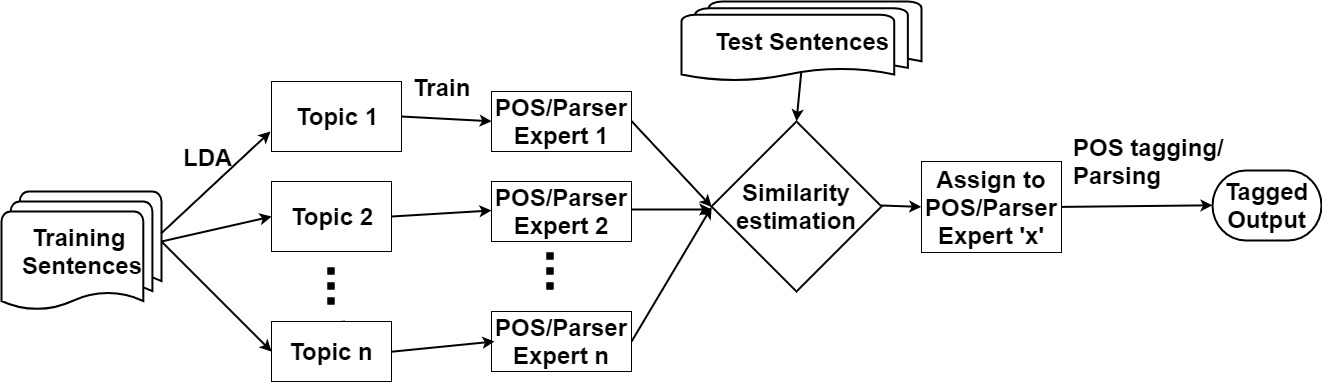
\includegraphics[width=\textwidth]{figures/approach-new.jpg}
 \caption{Overview of the architecture of the POS tagging and parsing experts.}\label{fig:architecture}   
 \end{figure*}



%\subsection{Background}

%not sure if this goes as a part of the problem statement

%In (ANONYMOUS), we create domain experts for POS tagging and parsing of heterogeneous datasets. We use Latent Dirichlet Allocation (LDA)~\cite{Blei:2003:LDA:944919.944937,Blei:2012:PTM:2133806.2133826} which identifies the hidden topic structure in a document. They have treated each sentence as a document. Thus, for each sentence, there is a probability distribution of topics. The sentences are clustered into the most likely topic based on the probability for training as well as the test set. While this approach effectively clusters training and test sentences into appropriate genre expert, it requires the topic modeler to be re-executed every time it encounters a new test sentence. We explore this problem of assigning a test sentence to the genre expert by using similarity metrics. Thus, in our approach, a test sentence gets automatically assigned to the genre expert it is closest to. This asynchronous assignment of test sentences to experts eliminates the requirement to run the topic modeler for each new test sentence. 


%\subsection{Problem description} 


%Following our previous work, we use LDA~\cite{Blei:2003:LDA:944919.944937,Blei:2012:PTM:2133806.2133826} to generate genres and train genre experts. But then, instead of having the test sentences clustered along with the training sentences, we assign test sentences to the genres via \textit{similarity metrics}. The test sentences are consequently annotated by the corresponding genre expert. The complete architecture of our approach is shown in Figure~\ref{fig:architecture}.

The training part of the process remains same as shown in figure~\ref{fig:architecture0} - LDA~\cite{Blei:2003:LDA:944919.944937,Blei:2012:PTM:2133806.2133826} is used to generate genres and train genre experts. In this chapter, I focus on the 2-topics case, which is the closest approximation for the mixed domain problem. Since in this case, we observed the best performance using hard clustering, I will use this as the base setting for similarity estimation experiments. 
I use 2 topics as prior, parallel to the 2 domains, and assign each training sentence via hard clustering to the genre for which LDA showed the highest probability.%\footnote{We have experimented with more topics for POS tagging and shown that we reach good results when using soft clustering rather than hard clustering \cite{mukherjee-kubler-scheutz:2016:W16-63}. The same holds true for experiments within the Penn Treebank, where we model WSJ internal topics, which are less distinct in their textual characteristics, but the experts still show an improvement over a full training baseline.}.  
I then test the different similarity metrics: I compute the similarity of a test sentence to the training sentences of the individual experts and then assign the sentence to the expert for tagging/parsing for which it has the highest similarity. I use the following similarity metrics:

\begin{itemize}
	\item Topic words from LDA: LDA does not only cluster sentences into genres, it also determines which words are highly correlated with each genre. Thus, we can utilize these words along with their probabilities for a specific genre. I sum over all genre words that we find in the sentence, weighted by their probability, and then assign the sentence to the topic that has the highest score. 
	
	\item $k$-nearest neighbors: There exist a wide range of metrics to calculate similarity between two feature vectors. However, since I compare a sentence to a set of genre sentences, I decided to use memory-based classification using the  $k$-nearest neighbors to classify each test sentence into the relevant class (or genre, in our case). This has the advantage over a pure similarity metric that we have a principled way of handling the comparison to a set of sentences. Additionally, I do not consider the whole search space, as I would if I used a centroid.
		\item Perplexity: Another obvious choice for determining the similarity of a sentence to a set of sentences is language modeling.  I calculate the perplexity of a test sentence with regard to set of sentences of an expert. I then assign a sentence to the expert for which it has the lowest perplexity. 
\end{itemize}



% \section{Related Work} \label{relatedwork}

% Our work cannot exactly be called domain adaptation since we automatically determine a range of genres and then train experts per genre while domain adaptation starts from a general model and adapts it to a specific genre. However, the two research questions are closely related and generally face the same problems. Our work is closest to the work by \newcite{plank2011effective} and \newcite{mcclosky:charniak:ea:10}. McClosky et al.\ address the problem of parse adaptation in the case of multiple sources. In their setting, a parser learns the domain differences and various statistics from being trained on datasets from multiple domains. Our approach is comparable to the extent that both approaches profit from a range of domains. \newcite{plank2011effective} adopt an approach where they build a highly specialized training set that is most similar to an  out-of-domain document. They create a specialized expert each time the parser encounters a new document. Our approach is more general than Plank and van Noord's in that we do not create an expert for every new document, but rather create experts per genre. In contrast,  our approach is more fine grained in that we assign individual sentences to genres rather than complete documents. \newcite{plank2011effective} use the topic distribution from LDA as features for determining the most similar training set. This is comparable to our approach of assigning test sentences to the proper genre (but not to the creation of genres). 

% Domain adaptation has been studied more extensively in parsing than in POS tagging.  For POS tagging, \newcite{blitzer:mcdonald:ea:06} have a similar setup to ours, where they train on WSJ data and test on MEDLINE abstracts. They use structural correspondence learning by identifying ``frequently occurring" pivot features which can appropriately represent source as well as target domain. The problem of adapting to a new domain is compounded in cases where no adequate data from the target domain is available. Differences in annotation scheme between the source and target domain can pose additional challenges \cite{dredze2007frustratingly}. In our case, GENIA follows a similar annotation scheme as WSJ with a few differences in assigning POS  tags to names. 

% Agreement based approaches and co-training have been employed for domain adaptation of POS tagging. In the agreement-based method adopted by \newcite{clark:curran:ea:03}, a Markov model tagger and a maximum entropy tagger are used. For a sentence to be included in the training set, both the taggers have to reach a unanimous decision. \newcite{sagae2007dependency} apply a similar approach but using MaxEnt and SVM to simulate an iteration of co-training. \newcite{kuebler:baucom:11} extended this further by demonstrating that an agreement in terms of word sequences rather than complete sentences is more robust and achieves better results.

% In the CoNLL 2007 shared task on domain adaptation for dependency parsing, 
% \newcite{attardi2007multilingual} adapt an error correction approach to revise mistakes caused by the base parser in the target domain. \newcite{kawahara2008learning} employ a single parser approach using a second order MST parser and combining labeled data from the known domain with unlabeled data of the new domain by simple concatenation and judging the efficacy of the resulting most reliable parses.
% \newcite{Finkel:2009:HBD:1620754.1620842} devise a  model for dependency parsing by using a hierarchical Bayesian prior based on the  notion that different domains may have different features specific to each domain.  Instead of applying a constant prior over all the parameters,  a hierarchical Bayesian global is used. 




\section{Similarity Estimation}\label{sim}
   
There are different ways of determining the similarity of a sentence to the sentences in a genre. We investigate methods based on the topic words from LDA, $k$-nearest neighbor approaches, and  perplexity.

\subsection{Topic Words from LDA}


LDA provides a list of the words most closely associated with a topic and assigns a weight to each word.  Thus, we can use the words that are highly correlated with each topic as good indicators for a sentence belonging to the genre represented by the topic. Additionally, we utilize the probabilities provided by LDA as weights to determine a word's contribution to the similarity. For this experiment, we select the top 50/100/200 words from each topic. I.e., we assume that these words can be considered to be the most representative  words in their respective domain. Then, for each sentence, we check how many of those words occur in the current sentence and add up their weights. 
We then assign the sentence to the topic with the higher value. Since we only look at a small number of words, we have to consider the cases where a sentence does not contain any of the topic words. We resolve these cases by extending beyond the top  words and considering all the words in the training set for each genre. If there is a tie in values, we assign the sentence randomly to one of the experts. 
\atrcomments{TBD: expand}

\atrcomments{Do I need to cite knn, dice coeff, ig/gain ratio,perplexity?}
\subsection{$k$-Nearest Neighbors}

In this method, I perform $k$-nearest neighbor classification to assign test sentences to topic experts. 
$k$-nearest neighbor is a supervised, non-parametric lazy learning algorithm. The typical steps for the algorithm is given as follows:

\begin{itemize}
    \item  The training data is stored in memory as feature vectors and associated class labels.
    \item The value of $k$ can be determined on a validation set based on the training errors for different $k$.
    \item For each datapoint in test, we do the following:
    \begin{itemize}
        \item We calculate the distance between the datapoint and each training data vector. Usually there are several metrics such as Euclidean distance, Cosine Similarity, etc.
        \item We sort these distances and consider the top $k$ values. 
        \item We choose the most frequent class from these and return it to be the predicted class for the test datapoint.
    \end{itemize}
\end{itemize}

\paragraph*{$k$-Nearest Neighbors as similarity metric}
I create a feature vector by using the top 50/100 words from each genre, as determined by LDA, and assigning the weights as values. The class label is the domain-membership, i.e., either WSJ or GENIA.

The classification parameters are determined by tuning these on a validation set. The settings are shown in table~\ref{tab:parameters}. It is based on the setting which had least training/validation errors. I explain these metrics in the next paragraphs.

\begin{table}[t]
\centering
\begin{tabular}{c|c|c|c}
\begin{tabular}[c]{@{}c@{}}Feature Vector\\  Size\end{tabular} & \begin{tabular}[c]{@{}c@{}}Number of\\ Nearest Neighbor\end{tabular} & Distance Metric & Feature Weighting \\ \hline
50 & 7 & Dice Coefficient & Gain Ratio \\
100 & 3 & Dice Coefficient & Gain Ratio \\ \hline
\end{tabular}
\caption{Classification parameters for $k$-nearest neighbors}
\label{tab:parameters}
\end{table}

\paragraph*{\textit{Dice Coefficient}}

Dice coefficient computes the similarity between two samples. In terms of set theory, this can be shown as:

\begin{equation} \label{eq:dc}
    DC(X,Y) ={\frac {2|X\cap Y|}{|X|+|Y|}}
\end{equation}

For language, dice coefficient can be used to calculate the number of common occurrences of character bigrams in the strings. Thus, given two strings $x$ and $y$, \ref{eq:dc} can be rewritten as:
\begin{equation}
    DC(x,y) = \frac{2n_{x \cap y}}{n_x + n_y}
\end{equation}

where $n_x$ is the number of character bigrams for string $x$ and $n_y$ is the number of character bigrams for string $y$.
Since we need to measure dissimilarity/distance rather than similarity, our metric is computed as below:
\begin{equation}
    d(x,y) = 1 - { \frac{2n_{x \cap y}}{n_x + n_y}}
\end{equation}

\paragraph*{\textit{Gain Ratio}}

In the previous paragraph, I discussed Dice Coefficient as the distance metric used in $k$-NN. However, it is a naive assumption that, all features are equally predictive of class labels. In other words, there are some features which are more informative than others. If we assume all features weigh same, we disregard this concept. Hence it is important to weigh features based on their predictive power. 

One of the widely used weighting scheme is Information Gain (IG). It measures how informative a feature is, to determine the class label. It relates to entropy which measures the amount of ``randomness" or uncertainty in a probability distribution. Entropy is represented as:
\begin{equation}
   H(Y) = -\sum_{y \in Y}  p(y)logp(y) 
\end{equation}
where $Y$ is a random variable. In this case, $Y$ can be considered as set of class labels such that $y \in Y$. 
Now, when we have the information on the value of the feature, we can compute a conditional entropy as below. 

% H(Y | X) = Si p(xi) H(Y | X=xi)
% H(C|v) = p(v) H(C|v) 
\begin{equation}
    H(Y|x) = \sum_{x \in X_n} p(x)H(Y|x)
\end{equation}

where $X_n$ is the value of the $n$-th feature.


Therefore, we can define information gain as difference between the overall entropy and the entropy conditional on the value of the feature. 

\begin{equation}
    IG(Y,x) = H(Y) - H(Y|x)
\end{equation}

While it is one of the commonly used metric, information gain tends to bias towards features with greater number of values i.e., the multi-valued features. Thus, a feature which is a good indicator of class label but contains lower number of values could potentially not given enough importance in information gain. To counter this effect, gain ratio is introduced, which normalizes information gain using a value referred to as split information (SI). This measures entropy on the value of the features. Thus SI is given as:
\begin{align}
    SI(n) = - \sum_{x \in X_n} p(x)logp(x)
\end{align}
Gain ratio can be represented as following:
\begin{align}
    Gain\ ratio = \frac{IG(Y,x)}{SI(n)}
\end{align}


\subsection{Perplexity-Based Similarity}

As the third set of methods, I turn to language modeling and use perplexity as a measure to determine the similarity. First, I explain the concept in details followed by the implementation details for using perplexity as a similarity measure.

\paragraph*{Probabilistic Language Models}

Language models assign probabilities to the sequence of words in a sentence~\citep{jurafsky2014speech}. It is essential to compute the most likely word that follows a sequence of words. N-gram is the simplest language model, which is a sequence of n words. We define a unigram, bigram and a trigram are sequences of one, two and three words respectively. If we consider a sentence to be a sequence of consequtive words,  $S = {w_1,w_2,...,w_n}$, the primary goal of a language model is to estimate the following:
\begin{align}
    P(S) = P(w_1,w_2,..w_n)
\end{align}
According to the chain rule of probability, we can calculate this as:
\begin{equation}
    \begin{aligned}
        P(w_1,w_2,..w_n) &= P(w_1)P(w_2|w_1)P(w3|w_1,w_2) ... P(w_n|w_1,..w_{n-1})&&\\
     &= \prod_i P(w_i|w_{1}^{i-1})&&
    \end{aligned}
\end{equation}

So, in order to find n-th word, we can simply estimate, $P(w_n|w_{n-1}, w_{n-2}, ... w_1)$. However, estimating conditional probabilities for sequences of any length is intractable and it is also nearly impossible to see all the probable sequences in the training data. Thus, it does not generalize well. Hence, we can make the Markov assumption, i.e., the future state depends on the current state only. In terms of language, this translates as:
\begin{align}
    P(w_1,w_2,..w_n) \approx \prod_i P(w_i|w_{i-k}..w_{i-1})
\end{align}

For a bigram model, we can make the following approximation:
\begin{align}
 P(w_i|w_1,w_2,..w_{i-1}) \approx P(w_i|w_{i-1})
\end{align}

We use maximum likely estimates (MLE) to calculate these probabilities. Hence,
\begin{align}
    P(w_i|w_{i-1}) = \frac{Count(w_{i-1}w_i)}{Count(w_{i-1})}
\end{align}

This means that, we calculate bigram probability of a word $w_n$, given the previous word $w_{n-1}$ by counting the number of times these words appear in conjunction in our corpus, normalized by the number of times $w_{n-1}$ appears in the corpus. 
Once we know these probabilities, it is trivial to estimate the most likely word that follows a sequence of words.  

\paragraph*{Evaluation of Language models - Perplexity}

There is an extrinsic evaluation method for language models, i.e., we use language model and then measure the end to end performance of a system. E.g., if we want to use language models for a machine translation system, we can judge the efficiency of using language model by simply evaluating the MT system. However, I discuss one of the widely used intrinsic evaluation method, perplexity. Perplexity is a function of probability of a sentence - it computes the inverse probability for an unseen test set, normalized by the number of words~\citep{jurafsky2014speech}. Hence, lower the perplexity, higher the probability, which implies that the model generalizes well.


\begin{equation}
    \begin{aligned}
    Perplexity(S) & = P(w_1,w_2,w_3, ... , w_n)^{-\frac{1}{n}} \\
    & = \sqrt[n]{\frac{1}{P(w_1,w_2,w_3, ... , w_n)}} \\
    & = \sqrt[n]{\prod_{i=1}^{n}\frac{1}{P(w_i|w_1, .. w_{i-1})}} \\
    \end{aligned}
\end{equation}
Thus, for bigrams, we can compute perplexity as:

\begin{equation}
    Perplexity(S) = \sqrt[n]{\prod_{i=1}^{n}\frac{1}{P(w_i|w_{i-1})}}
\end{equation}
    
\paragraph*{Perplexity as a similarity metric}

In the previous paragraph, we learned that perplexity can be a quick way to evaluate language models. I use perplexity as a measure to determine the similarity of a sentence to the training sentences. I have two training experts\footnote{See previous chapter for detailed explanation}, specializing in both domains in question. I calculate the perplexity of a test sentence to the experts. I then assign this test sentence to the expert which exhibits lower perplexity. I estimate unigram, bigram and trigram perplexity. 



\section{Experimental Setup} \label{exptsetup}

\subsection{Dataset}

We create our corpus manually by combining the Wall Street Journal (WSJ)~\cite{marcus:kim:ea:94} section of the Penn Treebank and the GENIA corpus~\cite{tateisi:tsujii:04}. This gives us an artificial balanced corpus for which we know to which genre a sentence belongs.  While WSJ consists of newspaper reports, GENIA consists of biomedical abstracts from Medline.


For the WSJ corpus, we use the POS annotation and syntactic annotations  from the treebank. The GENIA Corpus is annotated on different linguistic levels, including POS tags, syntax, coreference, and events, among others. We use GENIA 1.0 trees~\cite{Ohta:2002:GCA:1289189.1289260} created in the Penn Treebank format\footnote{http://nlp.stanford.edu/~mcclosky/biomedical.html}. Both treebanks are converted to dependencies using pennconverter~\cite{johansson2007a}.

Following our data split in \newcite{mukherjee-kubler-scheutz:2016:W16-63,E17-1033}, we create a balanced dataset comprising 17~181 sentences from each corpus for the training set and 850 sentences for the test set. Since GENIA is rather small and since there is no standard data split for GENIA, we decided to extract the last 850 sentences for the test set, and the 850 sentences before that for the validation set. The remaining 17~181 sentences are used for training. For WSJ, we chose the same number of sentences for the training, validation,  and test set, the training sentences are selected randomly from sections 02-21 and the validation and test sentences from section 22 and 23 respectively.


\subsection{Baselines}

In \newcite{mukherjee-kubler-scheutz:2016:W16-63,E17-1033}, we have used two baseline cases: The first baseline considers the entire training set and does not employ any topic modeling. Since the topic experts have access to only a fraction of the data, a second and more comparable baseline consists of  randomly distributing  training and test sentences into sets that correspond in size to the genres. We use these baselines and add a third, which is more relevant to our current setting. In this case, we use the experts trained on the genres but then randomly assign test sentences to the experts. This allows us to gauge how important a correct assignment to the corresponding expert is. 

\begin{table*}[t!]
\centering
\begin{tabular}{l|l|r|}
Similarity metric & Setting & Accuracy \\ \hline
joint LDA & & 98.94 \\ \hline
topic words & 50 & 97.59 \\ 
 & 100 & 97.53 \\ 
 & 200 & 97.35 \\ \hline
perplexity & unigrams & \textbf{99.76} \\ 
 & bigrams & 84.71 \\  
 & trigrams & 81.53 \\ \hline
$k$-NN & 50 & 90.59 \\ 
 & 100 & 91.18 \\ \hline
\end{tabular}
\caption{Accuracy of genre assignment for different similarity metrics.}
\label{tab:acc:class:simmetr}
\end{table*}


\subsection{Topic Modeling}

Probabilistic topic modeling is a class of unsupervised algorithms which detects the thematic structure in volumes of documents \cite{Blei:2012:PTM:2133806.2133826}. We use Latent Dirichlet Allocation (LDA),  a generative probabilistic model that approximates the underlying hidden topical structure of a collection of texts based on the distribution of words in the documents \cite{Blei:2003:LDA:944919.944937}.

We   use   the   topic   modeling   toolkit   MALLET  \cite{McCallumMALLET}.    The  topic  modeler  in MALLET implements Latent Dirichlet Allocation  clustering  documents  into  a  predefined number of topics.

\subsection{POS Tagging and Parsing}

For part of speech tagging, we use the Markov model POS tagger TnT (Trigrams'n'Tags) \cite{brants:00.2}. We use TnT mainly because of its speed and because it allows the manual inspection of the trained models (emission and transition
frequencies).
For the parsing experiments, we use the dependency parser of the MATE Tools\footnote{code.google.com/p/mate-tools}, a Java implementation of a graph-based parser~\cite{bohnet:2010:PAPERS}. For the parsing experiments, we use gold POS tags.



\begin{table*}[!t]
\centering
\begin{tabular}{l|l|r|}
Setting & Similarity metric & Accuracy \\ \hline
full training &  & 96.69 \\ 
random split & & 96.41 \\ 
topic experts + random test &  & 91.36 \\ \hline
joint LDA &   & 96.95 \\ \hline
topic words & 50 & 96.80 \\ 
 & 100 & 96.81 \\ 
 & 200 & 96.81 \\ \hline
perplexity & unigrams & \textbf{96.92} \\ 
 & bigrams & 95.64 \\
 & trigrams & 95.22 \\ \hline
$k$-NN & 50 & 96.05 \\  
 & 100 & 96.09 \\ \hline
\end{tabular}

\caption{Results for the POS tagging experiments.}
\label{tab:overallresultspostag}
\end{table*}



\subsection{Similarity Estimation}

For the $k$-nearest neighbor estimation, we use the Tilburg Memory-Based Learner (TiMBL) \cite{daelemans:zavrel:ea:10}. For the perplexity models, we derive $n$-grams  of the training experts using  Laplace smoothing, in NLTK~\cite{bird2009natural}, and compute the perplexity of the training experts to a test sentence.

\subsection{Evaluation}

We use the script \texttt{tnt-diff} that is part of TnT to evaluate the POS tagging results  and the CoNLL shared task evaluation script\footnote{http://ilk.uvt.nl/conll/software/eval.pl} for evaluating the parsing results.


\section{Experimental Results} \label{exptres}

\paragraph{Genre Assignment.}
We first investigate how well the different similarity metrics can assign the test sentences to the correct genre. I.e., we calculate accuracy in terms of whether a GENIA sentence is assigned to the GENIA genre, and a WSJ sentence to the WSJ genre.
Table~\ref{tab:acc:class:simmetr} shows the results of classification accuracy of using different similarity estimation techniques. The reference here is the joint LDA for training and test data, with an accuracy of 98.94\%. 
 
Perplexity based on unigrams reaches the highest accuracy, reaching an accuracy of 99.76\%, thus surpassing the joint LDA. Surprisingly, using bi- or trigrams instead decreases accuracy by 15-20 points absolute. We assume that this is due to data sparsity since the language model is trained on a relatively small dataset. The second highest accuracy is reached by the methods based on topic words. Here, the number of words considered does not seem to make a significant difference. The $k$-NN approach performs at around 91\%. These results indicate that using single words without context (i.e., the context in bi- and trigrams) provides the most reliable information. The language model has an additional advantage, potentially because it can smooth over unseen words.
  
  \begin{table*}[t!]
\centering
\begin{tabular}{l|l|rr|}
Setting &Similarity metric & LAS &UAS \\ \hline
full training & & 88.67 & 91.71 \\ 
random split &  & 87.84 & 90.86 \\ 
topic experts + random test &  & 82.17 & 88.13 \\ \hline
joint LDA & -& 90.51 & 92.14 \\ \hline
topic words & 50 & 90.30 & 92.07 \\
 & 100 & 90.30 & 92.07 \\
 & 200 & 90.30 & 92.07 \\ \hline
perplexity & unigrams & \textbf{90.54} & \textbf{92.16} \\
 & bigrams & 88.33 & 91.13 \\
 & trigrams & 87.50 & 90.68 \\ \hline
$k$-NN  &50 & 89.45 & 91.82 \\
 & 100 & 89.52 & 91.84 \\ \hline
\end{tabular}
\caption{Attachment scores for the dependency parsing experiments.}
\label{tab:overallresultsdep}
\end{table*}


  
\paragraph{POS Tagging.}
Table~\ref{tab:overallresultspostag} shows the accuracies of the POS tagging experiments for different similarity metrics. We notice that assigning the test sentences randomly to genres has a detrimental effect, and we reach an accuracy of 91.36\%, which is more than 5 points absolute lower than the random split baseline. This difference shows how important it is that sentences are assigned to the correct genre.
 
Perplexity based on unigrams and the method using topic words reach comparable accuracies to the original topic expert results based on the joint LDA clustering. These results follow the same trends as the genre assignment accuracies, but the differences between the methods are smaller. The perplexity setting using unigrams does not only surpass the joint LDA scores but also all the baselines: by nearly 0.3 percent points for the full training set, by 0.5 percent points  for the random split, and by 5 percent points  for the random test assignment.

\begin{table*}[t!]
\centering
\begin{tabular}{ll|rrr|}
 & setting & Correct genre & Incorrect genre  & Overall \\ \hline
POS tagging (acc.) & unigram & 96.92 &  91.84 & 96.92\\
&  topic words 50 & 98.23 & 88.59 & 96.80\\
parsing (LAS) & unigram& 90.54& 85.72 & 90.54  \\
& topic words 50 & 90.55 & 76.19 & 90.30\\ \hline
\end{tabular}
\caption{Results for POS tagging and dependency parsing when we separate incorrectly assigned sentences from correct ones.}
\label{tab:comp}
\end{table*}



\paragraph{Dependency Parsing.}
Table~\ref{tab:overallresultsdep} shows labeled and unlabeled attachment scores of the dependency parses. These results mirror the trends in the POS tagging experiments: Randomly assigning sentences to genres results in the lowest LAS score of 82.17\%, and using perplexity based on unigrams reaches the highest LAS of 90.54\%. This LAS is considerably higher than the full training baseline of 88.67\%. Note that the differences between the accuracies based on different similarity metrics are considerably more pronounced than in the POS tagging experiments. This mirrors the trend that we have previously seen for the joint LDA assignment. It is also interesting to see that the results for all the topic word settings are the same. This is due to 5 sentences that did not contain any of the topic words and thus had to be randomly assigned to one genre. 

We now have a closer look at the two best settings, i.e., the perplexity experiment using unigrams and 50 topic words: We separate the sentences that were assigned to the wrong genre from the correctly assigned ones and evaluate them separately. For the unigram setting, 4 sentences were assigned to the wrong genre, for the 50 topic words, 41 sentences. The results are shown in Table~\ref{tab:comp}.  These results show that the sentences that were assigned to the wrong genre receive POS and dependency analyses with significantly lower accuracies, the difference to the correct ones ranging between 5 points absolute for POS tagging and 10-14 points for parsing. This corroborates our findings that the correct assignment to a genre is of utmost importance, which also corroborates our conclusion that the genre experts model genre-specific information. If they did not, mis-assigning sentences would not have any impact.

\section{Discussion} \label{conc}

Using topic modeling to create experts can be very beneficial, but this approach is only viable if we can assign new sentences asynchronously to genres without having to retrain the LDA to determine genres that include the new sentences. We have investigated similarity based methods for assigning the new sentences to genres.
More specifically, we have  investigated the following methods:  1) using topic words that LDA associates with a genre, 2) $k$-nearest neighbor models, and 3) perplexity in language models. A baseline that assigns test sentences randomly to genres performs poorly, thus showing that the correct assignment to genres is indispensable.

Our results show that the perplexity model  based on unigrams surpasses the accuracy of a joint LDA model that assigns the sentences synchronously.  For POS tagging, the  accuracy of the unigram perplexity model is very close to that of the joint LDA.  For parsing, the unigram perplexity model outperforms the joint LDA model.  Using the 50 topic words to assign sentences to their genre reaches accuracies close to the best performing model. This shows that word-based methods are more robust in comparison to bigram and trigram methods, which should be able to profit from more context but also face data sparsity issues.

For the future, we plan to investigate models with a more dynamic mix of genres during the POS tagging and parsing process. I.e. rather than creating independent experts, we will investigate methods to create a POS tagger and parser that have access to expert views during each decision about the next POS tag or parsing step. We will also investigate whether we can integrate gold POS tags or dependency information into the topic modeling process, so that the topic modeler has access not only to the specialized lexical information but also to the linguistic information that it is ultimately tasked to distinguish. 


%%%%%%%%%%%%%%%%
% Chapter 7 - TBL
%%%%%%%%%%%%%%%%

\chapter{Transformation-based Error-driven Learning in Dependency Parsing}

\section{Introduction}
\label{sc:main}

Dependency parsing results tend to be reliable as long as the parser is trained and tested on data from a single domain. However, the situation is considerably more challenging when the data set on which the parser is tested/used is different from the sentences on which it is trained. For example, a parser trained on newspaper corpus would not parse texts based on spontaneous dialogues accurately. Since it is impossible to manually annotate the amount of data needed to train a parser in any domain that we need to parse, we need automatic methods to adapt a parser to those new domains. %Manual annotation is even harder when the syntactic structure of the data differs widely. E.g., the syntactic structure of a newspaper corpus is very different from that of natural language dialogue corpus or literary works. This leads to significant differences in the way these corpora are annotated to capture these inherent differences. 
%%SK: that is not true, theoretically, you can use the same scheme, but practically there are phenomena in the target domain that are important, but you definitely cannot introduce this as an integral part of domain adaptation.
This problem is generally addressed in domain adaptation. Domain adaptation attempts to use a large set of annotated data from a different domain plus specific strategies to adapt the annotations to the target domain, for which a small amount of annotated data may exist. The problem is compounded when there are differences in the annotation schemes between the source and target domain. Different treebanks, representing different domains, tend to  use somewhat different annotations \cite{dredze2007frustratingly}. These differences can be due to individual syntactic interpretations of different annotators, but in many cases, they are necessitated by phenomena in the target domain that do not exist in the source domain. Spontaneous dialogues, for example, have a large number of incomplete sentences with words that cannot be attached easily if their head is missing (e.g., the determiner in ``I bought the -'').
%This is because the parser learns the syntactic constructions from the source domain corpus, i.e., the newspaper corpus in this case, which does not always apply to the target corpus, the dialogue corpus. Hence, these differences leads to incorrect structural as well as functional errors or both. Structural errors affect the structure of a parse tree, i.e., when the head of a dependency arc is predicted incorrectly affecting the unlabeled attachment scores. Inaccurate prediction of the label of the arc results in functional errors. This lowers the labeled attachment scores as well as label accuracy. 

Out-of-domain dependency parsing results tend to be low as compared to in-domain results. The problem can be looked at from different perspectives. Previous work in this area has extensively looked at the structural errors, where the dependency arcs are corrected. For instance, the DeSR parser~\cite{attardi2007multilingual, attardi2007tree, attardi2009accurate} implements tree revisions. %, i.e., the mistakes made by the base parser for the target domain are rectified by the tree revision method. I.e., the change is at a structural level where the dependency arcs are moved to a different head in the dependency tree. 
Structural change of dependency trees prove to be an effective domain adaptation method. %The method improves the unlabeled attachment scores (UAS). 
\citet{yu2015domain} report a 1.6\% improvement by using self-training to generate training examples for the target domain. To our knowledge, no methods have been reported addressing functional errors, i.e., errors in the dependency labels.

Our work focuses on a target domain of spontaneous dialogues, using the CReST Corpus \citep{eberhard2010indiana}, %Here, the situation is complicated by the fact that 
which uses labels that do not occur in the source domain corpus. We propose to use 
%apply a method which could reduce structural as well as functional errors. In this paper, we look at functional errors. Functional errors originating from the difference in dependency labels between source and the target domain contributes to a significant reduction in the labeled attachment scores. This is evident when the source and target domains have different number of dependency labels. E.g., the target domain could have a subset of source domain labels. In that case, a parser trained on source domain would parse a sentence from target domain differently leading to a drop in LAS. The problem is equally challenging for the other scenario, where source has a subset of target labels. In that case, the parser has not seen the labels in the source and it will almost certainly parse it wrong. 
transformation based error driven learning (TBL) \cite{Brill:1995:TEL:218355.218367} to address the problem. The method has been proven effective in a variety of NLP problems including POS tagging and syntactic parsing. The idea is simple:  We use a small annotated data set in the target domain and automatically annotate it using a source domain parser.  Our goal to learn a set of rules from the errors that occur and a set of rule templates. 
%We emulate this approach with modifications to learn rules by applying transformations to a text annotate by a parser trained on a different domain. Our method rectifies the errors in dependency labels even in the case where a particular label doesn't appear in source. Thus, it greatly improves the labeled attachment score. The main advantages of this method are - it only requires a small amount data for training and it is easily generalizable for any domain. 
Although we focus on correcting dependency labels in the current paper, our method can be extended to correct the errors in dependency arcs as well.
%In this paper, 
We demonstrate that using TBL with a small target domain training set improves dependency parsing accuracy by about 10 \% absolute, and it learns to use the target-specific labels. 

The paper is structured as follows: Section~\ref{sec:related} discusses related work, section~\ref{sec:background} describes the issues in domain adaptation in more detail, and section~\ref{sec:tbl} explains our approach of using
TBL for domain adaptation. In section~\ref{sec:exptsetup}, we describe our experiment setup, and section~\ref{expt_results} discusses the results. Section~\ref{conclusion} concludes and delineates
future work.


\section{Related Work} \label{sec:related}

There has been a significant amount of work done on domain adaptation in dependency parsing. The primary challenge of domain adaptation is the unavailability of annotated examples from the target domain. Previous work in this area focused on analyzing how this affects parsing quality and on building systems to bypass the need for having a large amount of target domain data. Although distributional difference between the domains is a common problem,  in general, \citet{dredze2007frustratingly} conclude that domain adaptation is most challenging when there are dissimilarities in annotation schemes between the domains. %This was a part of their analyses based on the systems submitted for CoNLL 2007 shared task~\cite{nilsson2007conll}. 

Domain adaptation for dependency parsing was one of the tasks in the CoNLL 2007 Shared Task. %The multilingual track task was to learn from a training data and then parse test data from multiple languages. 
The shared task was focused on the scenario where there is no data available from the target domain. Out of the 10 systems participating in the domain adaptation task, the highest results (81.06\% LAS; 83.42\% UAS) are achieved by \citet{sagae2007dependency}. To add target domain sentences to the training set, they emulate a single iteration of co-training by using MaxEnt and SVMs, selecting the sentences where both models agreed. The system by \citet{attardi2007tree} (80.40\% LAS; 83.08\% UAS) produced similar results. They use a tree revision method~\cite{attardi2007tree} to correct structural mistakes. %Revision stands for moving a dependency arc to a different head in the dependency tree. 
They formulate the problem as a supervised classification task using a multiclass perceptron, where the set of revision rules is the output space and features are based on syntactic and morphological properties of the dependency tree. %They focus mostly on structural errors in their work. 

%Structural errors  have received much attention in domain adaptation for parsing, but functional errors, concerning dependency labels) have mostly been ignored. \shortcite{attardi2007multilingual} made an observation for Catalan for the multilingual track. The corpus provided by the shared task had 42 labels to standardize with the other corpora. However, the original Catalan had 195 labels. They experimented on Catalan corpus with the original 195 labels and then, the reduced 42 labels. They reported that the reduction from 195 to 42 labels for Catalan corpus decreased the LAS of the parser by nearly 4\%. Although this is a case of multilingual adaptation, this is comparable to our work because this shows that  the parser performance is negatively affected when the test set contains a subset of training set labels.
%%SK I am not sure if this can fall under domain adaptation, this is more about language internal annotation differences???


%not sure if this is needed -->
A popular approach for domain adaptation is selecting appropriate training data by using self-training or co-training for domain adaptation. Although testing on a single domain, \citet{McClosky:2006:ESP:1220835.1220855,McClosky:2006:RSP:1220175.1220218}  show the effectiveness of using reranking using self training. They achieved an improvement of around 1\% on unlabeled data. 
%\citet{kawahara2008learning} employed a single parser using second order MST Parser and combined labeled data from the target domain with unlabeled data of the source domain by 
%%SK:  this is still unclear 
%concatenation and judging the efficacy of the resulting most reliable parses. They use a binary classifier to estimate whether a parse is reliable, using features such as sentence length, dependency length, unknown words, punctuation, average frequency of words in a sentence. 
%For domain adaptation, they explore the concatenation of labeled and unlabeled data by concatenating unlabeled source domain data with labeled target for training. 
%They report a 1\% increase in accuracy over the contemporary state of the art CoNLL shared task results on the CoNLL 2007 shared task data.
\citet{kawahara2008learning} devised a method to select reliable parses from the output of a single dependency parser, MST parser~\cite{mcdonald2005non}, instead of using an ensemble of parsers for domain adaptation. 
%%SK: yes, but you still don't explain how the combination of labeled and unlabeled works -> they just say they concatenate 
They use a self training method and combine labeled data from target domain with unlabeled data from the source by ``concatenation''. To estimate whether a parse is reliable, they applied binary classification using SVM on features such as sentence length, dependency length, unknown words, punctuation, average frequency of words in a sentence. They report a 1\% increase in accuracy over the contemporary state of the art CoNLL shared task results on the shared task data.
%%
\citet{yu2015domain} applied self-training for domain adaptation using confidence scores to select appropriate parse trees. Their highest improvement in terms of LAS is 1.6\% on the CoNLL data. %Our approach can be considered somewhat analogous to the goal of this idea - we have some amount of labeled data from the target domain and we learn from the mistakes made in the target domain dataset by parsing it with a different source domain dataset. We then iteratively rectify these mistakes to create rules which would then eventually help parse texts from the target domain. 

\shortcite{blitzer:mcdonald:ea:06} used structural correspondence learning (SCL) for POS tagging and parsing to find ``frequently occurring'' pivot features, i.e., features that occur frequently in unlabeled data and equally characterize source and target domains. They used the WSJ as the source and MEDLINE abstracts as the target domain. They established that SCL reaches better results in both POS tagging and parsing than supervised and semi-supervised learning even when there is no training data available on the target domain. %We assume that we have a small amount of labeled training data available from the target domain for our current experiments.

Transformation based error driven learning (TBL) was originally developed for POS tagging \cite{brill1992simple,Brill:1995:TEL:218355.218367}.
\citet{brill1993automatic} also used this approach to parse text by learning a ``tranformational'' grammar. The algorithm repeatedly compares the bracketed structure of the syntactic tree to the gold standard structure and learns the required transformations in the process. \citet{brill1994rule} also use this technique for prepositional phrase attachment disambiguation.
%Brill's initial with the baseline which is the most frequent part of speech tags for a sentence. Then the model corrects the errors by applying the rules repeatedly. 
%This approach has been used by \citet{Nakagawa:2002:SBP:1118771.1118778}
%%SK: Correct? - they use revision learning, should i keep it?
%for POS tagging and term extraction, where they use a second classifier to determine the accuracy of the base parser. 
%atr: there is a paper which speeds up tbl for pos tagging
Transformation based error driven learning has also been used for information retrieval by \citet{woodley2005applying}.
%Our work is similar to this concept, since we attempt to correct an output parse from the target.
%%SK: Do you have more papers that use TBL for other problems? -x

% \shortcite{attardi2007multilingual} used a tree revision method~\cite{attardi2007tree} that corrects the mistakes caused by the base parser for the target domain. Revision stands for moving a dependency arc to a different head in the dependency tree. They formulated the problem as a supervised classification task using multiclass perceptron, where the set of revision rules is the output space. They use syntactic and morphological properties of a dependency tree. This method is similar to reranking~\cite{charniak2005coarse,collins2005discriminative}, which works by generating $n$-best parses of a given sentence. Then, with the help of global features and a discriminative models, the reranker trains on these parses. \shortcite{McClosky:2006:ESP:1220835.1220855,McClosky:2006:RSP:1220175.1220218} also showed the effectiveness of using reranking using self training. This is based on Brill's POS tagger~\cite{brill1992simple,Brill:1995:TEL:218355.218367} using transformation error driven learning, where he initializes with the baseline which is the most frequent part of speech tags for a sentence. Then the model corrects the errors by applying the rules repeatedly. This approach has also been implemented by \shortcite{Nakagawa:2002:SBP:1118771.1118778} for POS tagging, where they use a second classifier to determine the accuracy of the base parser. Our work is similar to this concept, since we attempt to correct an output parse from the target.

% There has been a significant amount of work done on domain adaptation in dependency parsing.
% The primary challenge of domain adaptation is the unavailability of examples from the target domain. Previous work in this area focused on analyzing how this affects the problem in question and on building systems to bypass the need of having substantial volume of target domain examples.

% The CoNLL 2007 shared task~\cite{nilsson2007conll} had two tracks: multilingual parsing and domain adaptation. 
% %%SK can you add info what the task was, how many systems participated in the second track, and what the overall results were?
% %%Are all the following papers from the shared task?

% %%SK OK, first of all why should we care? I would expect you to tell me about the system that had the best performance in the shared task?
% %%SK and the description is a bit confusing, what exactly did they do, and why is that multilingual domain adaptation? and what is case1?
% The DeSR parser by~\shortcite{attardi2007multilingual} had the best performance for Catalan for the multilingual task. The corpus provided by the shared task had 42 labels to standardize with the other corpora. However, the original Catalan had 195 labels. They experimented on Catalan corpus with the original 195 labels and then, the reduced 42 labels. They reported that the reduction from 195 to 42 labels for Catalan corpus decreased the LAS of the parser by nearly 4\%. Although this is a case of multilingual domain adaptation, this is comparable to case 1 because this shows that even within the same language, reduction in labels from training to test harms the performance of the parser. For the domain adaptation track, they used a tree revision method~\cite{attardi2007tree} which corrects the mistakes of the base parser and 
% %%SK would it kill you to tell us how much of an improvement they got? this should give the reader an understanding of how to interpret our findings, did we get a LOT of improvement, just a bit in comparison to other approaches? That is hard to do when they only know 'significant improvement', which can be in the range of 0.5--60ish? 
% noticed a significant improvement in the performance over baseline.

% %%SK: that is super relevant for our paper, and we only get the conclusion? Tell us a bit more
% \shortcite{dredze2007frustratingly} concluded that domain adaptation is more challenging when there are dissimilarities in annotation schemes between the treebanks.

% %%OK, here the focus should be on the fact that they do it without any annotated data from the target domain, and again tell us how much improvement? 
% \shortcite{blitzer:mcdonald:ea:06} experimented on structural correspondence learning (SCL) which focuses on finding ``frequently occurring" pivot features that occur commonly across domains in the unlabeled data but equally characterize source and target domains. Blitzer et al.\ used the WSJ as the source and MEDLINE abstracts as the target domain. They established that SCL reaches better results in both POS tagging and parsing than supervised and semi-supervised learning even when there is no training data available on the target domain.


% \shortcite{sagae2007dependency} emulate a single iteration of co-training by using MaxEnt and SVM, selecting the sentences where both models agreed and adding these sentences to the training set. Their approach reached 
% %% how much improvement?
% the highest results on the domain adaptation task of CoNLL 2007~\cite{nilsson2007conll}. 
% \shortcite{yu2015domain} applied a self-training based method for domain adaptation which employs confidence scores based method to select appropriate parse trees. Their highest improvement in terms of LAS, is 1.6\% on chemical texts. 

% %Towards Domain Adaptation for Parsing Web Data ~\cite{khan:dickinson:ea:13.2} 
% %Domain Adaptation for Dependency Parsing via Self-training ~\cite{yu2015domain}
% %Unsupervised Linguistically-Driven Reliable Dependency Parses %Detection and Self-Training for Adaptation to the Biomedical Domain ~\cite{dell2013unsupervised}

% \shortcite{kawahara2008learning} employed a single parser approach using second order MST Parser and combining labeled data from the unknown domain with unlabeled data of the known domain by 
% %%SK that may be simple but i have no ide ahwta they did?
% simple concatenation and judging the efficacy of the resulting most reliable parses. 
% \shortcite{Finkel:2009:HBD:1620754.1620842} devised a new model for named entity recognition as well as dependency parsing by using hierarchical Bayesian prior. This is influenced by the notion that different domains may have different features which is specific to each domain.  However, instead of applying a constant prior over all the parameters,  a hierarchical Bayesian global is used. This enables sharing of information across domains but also allows to override this information if there is ample evidence.
% \shortcite{mcclosky2010automatic} designed the problem as ``multiple source parse adaptation", in which a parser was trained on multiple domains and learned the statistics as well as domain differences which affects the parser accuracy. Their parser outperforms the state-of-the-art baselines. 

% %%SK well, yes, this comes a bit late?
% Domain adaptation was the task of the CoNll 2007 shared task. 
% \shortcite{attardi2007multilingual} used a tree revision method~\cite{attardi2007tree} that corrects the mistakes caused by the base parser for the target domain. Revision stands for moving a dependency arc to a different head in the dependency tree. They formulated the problem as a supervised classification task using multiclass perceptron, where the set of revision rules is the output space. They use syntactic and morphological properties of a dependency tree. This method is similar to reranking~\cite{charniak2005coarse,collins2005discriminative}, which works by generating $n$-best parses of a given sentence. Then, with the help of global features and a discriminative models, the reranker trains on these parses. \shortcite{McClosky:2006:ESP:1220835.1220855,McClosky:2006:RSP:1220175.1220218} also showed the effectiveness of using reranking using self training. This is based on Brill's POS tagger~\cite{brill1992simple,Brill:1995:TEL:218355.218367} using transformation error driven learning, where he initializes with the baseline which is the most frequent part of speech tags for a sentence. Then the model corrects the errors by applying the rules repeatedly. This approach has also been implemented by \shortcite{Nakagawa:2002:SBP:1118771.1118778} for POS tagging, where they use a second classifier to determine the accuracy of the base parser. Our work is similar to this concept, since we attempt to correct an output parse from the target.

% %%OK, overall you have enough related work, but it mostly reads like they did this, they did that, they did something like this ... That is very hard to read. Can you rewrite this section and try to focus more on how this relates to what we are doing?



\section{Issues in Domain Adaptation} \label{sec:background}

%The primary goal of our work is to address the problem that results from using a parser, trained on one domain to parse sentences from a different domain. The state-of-the-art parsers work predictably well on in-domain sentences, however, the accuracy suffers in case of out-of-domain sentences. In case of a dependency parser, accuracy results from predicting the dependency arc and the label correctly. In other words, the following cases cause the parser accuracy to decline.

%%SK I'm not sure if we should leave this in, We are throwing two different problems together. DOmain adaptation is really hard when you have no target data, it's easier in our setting with data.  
%% atr - may be we can keep it from the We will first analyze ...

%Domain adaptation for dependency parsing has received a fair amount of attention, as described above. It has acquired the reputation of being an extremely challenging problem, where only minimal improvements can be gained. In many cases in domain adaptation, a 1\% improvement is the state of the art~\cite{dredze2007frustratingly,mcclosky:charniak:ea:10,khan:dickinson:ea:13.2,yu2015domain}. One potential reason for this difficulty to gain more substantial improvements may lie in the fact that it is either treated in a holistic approach, or researchers focus on one specific part of the adaptation, which then limits the progress that can be made. 
%We will thus first analyze the problem to better understand the different facets of the problem. In a second step, we will suggest a solution that can handle all of those cases.

Before we present our approach to domain adaptation, we need to better understand the different facets of the domain adaptation problem. This analysis will motivate our solution, which can handle all of those cases.

\subsection{Error Types}

The first phenomenon that we look at is the types of errors that can occur in dependency parsing:

\begin{compactenum}
    \item Predicting the \textbf{head of a dependency arc} inaccurately, resulting in a structural error. %- this affects the structure and thus the unlabeled attachment score of the sentence.
    \item Predicting the \textbf{label of a dependency arc} wrong, resulting in a functional error. %this affects the overall labeled attachment score of the sentence.
    \item Predicting both \textbf{label and the head of a dependency arc} wrong, resulting in structural and functional problems.
\end{compactenum}

Note that structural errors affect the labeled and unlabeled attachment scores, functional errors only affect labeled attachment scores.

Previous work focused on correcting structural errors introduced by inaccurate prediction of the head of a dependency arc. %Thus these methods focus on structural changes. 
%One example is the DeSR~\cite{attardi2007multilingual,attardi2007tree,attardi2009accurate} parser, which is conceptualized domain adaptation as a tree revision procedure. %the procedure can be used to improve parses within a domain, out of domain, as well as in multilingual adaptation. 
%I.e., this method concentrates on correcting the dependency arcs, it does not consider labeling errors. 
To our knowledge, there are no approaches to address these functional errors.

% \begin{table}[!t]
% \centering
% \begin{tabular}{l|l|r}
% \multicolumn{2}{c|}{Cases} & Number of instances \\ \hline
 
% 1 & \multicolumn{1}{l|}{Incorrect Dependency Label} & 22~252 \\
% 2 & \multicolumn{1}{l|}{Incorrect Dependency Head} & 17~010 \\
% 3 & \multicolumn{1}{l|}{Incorrect Dependency Label \& Correct Dependency Head} & 12~405 \\
% 4 & \multicolumn{1}{l|}{Incorrect Dependency Label \& Incorrect Dependency Head} & 7~163 \\
% %5 & \multicolumn{1}{l|}{Correct Dependency Label \& Dependency Head } & 9~847 \\ 
% \hline
% \end{tabular}
% \caption{Analysis of sentences from GENIA corpus containing instances of incorrect dependency label prediction}
% \label{tab:initanalysis}
% \end{table}

\begin{table}[!t]
\centering
\begin{tabular}{l|l|r}
\multicolumn{2}{c|}{Cases} & \# instances \\ \hline
 
1 & \multicolumn{1}{l|}{Incorrect dependency label (incl.\ correct \& incorrect heads)} &  13~839\\
2 & \multicolumn{1}{l|}{Incorrect dependency head (incl.\ correct \& incorrect label)} &  10~294\\
3 & \multicolumn{1}{l|}{Incorrect dependency label \& correct dependency head} & 5~389 \\
4 & \multicolumn{1}{l|}{Incorrect dependency label \& incorrect dependency Head} &  8~450\\
%5 & \multicolumn{1}{l|}{Correct Dependency Label \& Dependency Head } & 9~847 \\ 
\hline
\end{tabular}
\caption{Analysis of sentences from CReST containing  incorrect dependency predictions.}
\label{tab:initanalysis}
\end{table}

Next, we need to determine how serious these problems are. We concentrate on a setting where the source domain is the WSJ part of the Penn Treebank \cite{Marcus:1994:PTA:1075812.1075835} and the target domain is the CReST Corpus \cite{eberhard2010indiana} (for more details on the corpora, see section~\ref{sec:exptsetup}). We now take a closer look at a parsing experiment where we use 17~181 WSJ sentences for training the MATE parser and 5~759 CReST sentences for testing. The different types of errors are shown in table~\ref{tab:initanalysis}.
This analysis shows that functional errors, i.e., errors involving dependency labels, are more frequent than structural errors. Thus, by ignoring those errors in domain adaptation, we artificially limit the possible improvements.


\subsection{Error Sources}

A second type of difference concerns the source of the parser errors. Here we need to distinguish two cases:

\begin{compactenum}
    \item Parser inherent errors, i.e., errors that the parser makes independent of the out-of-domain setting.
    \item  Parser errors caused by differences in distribution between the two domains.
    \item Differences in annotation, i.e., the domain data on which we evaluate differ from the annotations in the source data.
\end{compactenum}

In the following, we focus on the differences of type 2 and 3. More specifically, we work on errors in the dependency labels since these are easier to distinguish. Structural differences tend to be differences of degree, which are difficult to separate into distributional differences (type 2) and annotation differences (type 3). In order to establish whether annotation differences cause issues, We have analyzed a range of treebanks that are annotated using (variants of) the Penn Treebank label set. %Annotation differences The problem is especially evident when source and target domains differ in the number of dependency labels. This means that one treebank has labels which may or may not be present in the other.  If such differences exist, label confusion is prevalent and can cause a considerable drop in the Labeled Attachment Score. % which is a measure of the accuracy in identifying the head and the dependency relation between a pair of words in a sentence. 

\begin{table}[!t]
\centering
\begin{tabular}{l|c|c}
Treebank & No. of dep.\ labels & \begin{tabular}[c]{@{}c@{}}Intersection with WSJ\end{tabular} \\ \hline
WSJ & 67 & - \\
%GENIA & 22 & 22 \\
CReST & 31 & 22 \\
Brown & 71 & 60 \\ \hline
\end{tabular}
\caption{Differences in the dependency label sets across treebanks.}
\label{tab:depreldist}
\end{table}

Table~\ref{tab:depreldist} looks at differences in the dependency label sets in the following treebanks: the WSJ part of the Penn Treebank, the Brown Corpus \cite{francis1964brown} (Sections cg, ck, cl, cm, cn, cp, cr), 
%the GENIA corpus~\cite{tateisi:tsujii:04}, 
and the CReST Corpus \cite{eberhard2010indiana}.
The CoNLL style dependency trees of the WSJ and the Brown Corpus are created using the pennconverter tool \cite{johansson2007a}; CReST was natively annotated in dependencies as well as constituents.
It is obvious  that there are considerable  differences in the annotation schemes, especially between WSJ and CReST, which only have 22 labels in common.  We can establish three different scenarios:

\begin{compactenum}
    \item The source is a superset of the target data set.
    \item The source is a subset of the target data set, 
    \item Both the source and target annotations have labels that do not occur in the other data set.
\end{compactenum}

In the first case, the distribution of labels may be different between source and target, which can cause incorrect parsing decisions. The problem in the second case is more difficult since the parser is supposed to predict labels that it has not seen in training. The third case is a combination of the first two and thus the most difficult to handle.

Returning to our treebanks, we assume that since WSJ has the largest number of manually annotated sentences,  it will serve as the source domain. In this case,  CReST mainly shows a subset of labels from WSJ, but also has 9 labels that do not occur in WSJ. %Brown, in contrast, uses a superset of the WSJ labels. 

Our hypothesis is that we can address \textit{all} of the problems described above by using transformation based error driven learning~\cite{Brill:1995:TEL:218355.218367} (for a description of  this method see section~\ref{sec:tbl}). The method has been proven effective in many  tasks such as POS tagging, syntactic parsing, and machine translation. 
 
 %analysis results -->


 %We selected 5000 sentences randomly from the GENIA corpus which contain instances of incorrect dependency label prediction. Our initial analyses on these sentences are given in Table~\ref{tab:initanalysis}.


%\begin{table}[!htb]
%\centering
%\begin{tabular}{l|c} \hline
%Number of GENIA sentences %considered & 5000 \\
%Total number of tokens in these %sentences & 132776 \\ \hline
%\end{tabular}
%\caption{My caption}
%\label{my-label}
%\end{table}

For the work presented here, we will focus on cases where the parser has predicted an incorrect label. This is motivated by our findings in table~\ref{tab:initanalysis}, which show that label errors are more frequent than structural ones. %since there is a significant number of cases where dependency label has been predicted incorrectly (Case 1). This is also considerably higher than the number of cases where the head of the dependency arc is predicted incorrectly (Case 2). Number of instances where the label is predicted incorrectly but the head is accurately predicted (case 3) is also noticeably higher than the converse case (case 4). 
%Hence it is evident from our findings that addressing the problem of incorrect prediction of dependency label could be a substantial part in addressing the domain adaptation problem for dependency parsing, in general.
We investigate the scenario using CreST, where the source has a superset of  labels in the target annotations, but with some unique labels in the target annotations. We hypothesize that our method can lead to an improved performance of the parser on the target domain, including dependency labels that do not exist in the source treebank. We evaluate this by the Labeled Attachment Scores (LAS) and Label Accuracy (LA). %How we employ transformation based error driven learning~\cite{brill1992simple,Brill:1995:TEL:218355.218367} to bridge the gap between source and target domains is described in the next section.

\section{Transformation-Based Error-Driven Learning for Domain Adaptation} \label{sec:tbl}

\subsection{TBL: The Brill Tagger}

%%SK: can you rewrite this section?  -x
% 1) Integrate the first two paragraphs into one. 
% 2) You need to provide more details about how TBL works. The paragraph is too "theoretical", and the enumerated list not very useful without explanations. For example, you are not saying anywhere that the gold corpus and the unannotated text are the same text. Step 3 sounds like magic. No4: what is the initial system? 5: what rules? How may do you apply in each step, how do you choose them? 
% 3) I think it helps if you introduce the distinction between rule hypotheses and learned rules, but that is just me. 
% 4) I would also make the description more specific, i.e. focus on POS tagging; that tends to be easier to understand than a more general, less specific description.  
% 5) Explain what the templates are. here, focusing on pOS tagging will help. You should introduce the template notation here and then give 1-2 examples of POS templates.
% 6) And potentially move the figure into this section. If you lose your readers here, you won't get them to pay attention to the next section ....
%It wold also help if you asked a CL student to read this paragraph,to see if they understand it.

We implement the idea of transformation based error driven learning, which was originally developed by \citet{brill1992simple} for POS tagging. The method works with two versions of the training data: the gold standard and (an initially unannotated) working copy that simulates the learning process and records the errors. The unannotated version of the training data is tagged by a simple part of speech tagger\footnote{This could be any simple part of speech tagger, or a heuristic that labels every work with the most frequent POS tag}, to create the initial state of the working copy of the text.  The goal is to bridge the difference between the gold standard text and the working copy by learning rules that change the incorrect POS tags to the correct ones. 
%This is done by applying a set of rule templates repeatedly and computing the objective function. 

Learning is based on rule templates, which consist of two parts: rewrite rules and triggering environment. The templates need to be determined by the researcher, based on the problem. In general, a rule template is of the form:


\textbf{Rule Template} ${(A, B): X \rightarrow Y} $

I.e., if we observe conditions $A$ and $B$ (triggering environment), we change the output variable (POS tags, for Brill and dependency labels, for us) 
from $X$ to $Y$ (rewrite rule). Note that X can remain unspecified, then the rule is applied independent of the current variable (label or POS tag).

The following is an example of a rule template for POS tagging: Change the POS tag of the current word from X to Y if the previous word is tagged as Z, where X, Y, and Z are variables that need to be instantiated during learning. 

The learner creates rule hypotheses out of those templates by identifying incorrectly tagged words in the working copy and instantiating the template variables.
For example, one possible rule hypothesis could be the following: Change the POS tag of the word ``impact'' from verb to noun if the previous word is tagged as a determiner. %One such template can instantiate multiple transformations. 
%At each stage, a list of multiple transformations are instantiated by applying these templates. 

In one pass through the system, all possible rule hypotheses are created and ranked  based on an objective function which determines for each hypothesis how many corrections occur. The rule hypothesis with the highest score is applied to the working copy and added to the final list of transformations, stored in order, during the training process. Then the process repeats, and new rule hypotheses are generated from the templates based on the remaining errors in the working copy. The process finishes when there is no more improvement in terms of reduction of errors. %The process can be described as follows:

%Every time it finds an error in target, it instantiates the rules (from the templates) that it learns from the gold corpus and checks the resulting errors. It measures the improvement in terms of how many new errors are introduced as a result of the application of the rule. It rewards the rule with the most improvement and adds it to the set of learned rules. Hence, the next time a text from the same domain needs to be tagged, it can go through the set of learned rules and correct the errors introduced by parsing it using a model from a different domain. Thus it corrects itself based on what the gold data shows. The main advantage of this approach is that, it is flexible in terms of domain as well as multilingual cases.
%We describe the general approach for transformation based error driven learning as below.


% \begin{algorithm}
% 		\caption{Tranformation Based Error Driven Learning}
% 		\label{array-sum}
% 		\begin{algorithmic}[1]
% 			\Procedure{ArraySum}{$A$}
% 			\State $sum = 0$
% 			\For {each integer $i$ in $A$}
% 			\State $sum = sum + i$
% 			\EndFor
% 			\State Return $sum$
% 			\EndProcedure
% 		\end{algorithmic}
% \end{algorithm}

%%SK: are you changing this into the algorithm? - x
%\begin{enumerate} 
%    \item Input: 
%    \begin{itemize}
%        \item Initial state annotated text
%        \item Gold Corpus
%        \item list of templates (rules and conditions to trigger the rules)
%    \end{itemize}
%    \item Output: List of rules.
%    \item Learn possible transformation from the gold corpus based on the templates. 
%    \item Run the unannotated text through an initial system to get the initial state, i.e., the training set for the transformation based error driven learning.
%    \item Iterate over the initial state text and do the following until the number of errors cannot be reduced anymore:
%    \begin{enumerate}
%        \item Apply the transformations learned from the gold corpus
%        \item Compute the resulting errors caused due to application of a transformation.
%        \item Select the transformation with the least number of errors and add this to the final list of transformations.
%   \end{enumerate}
%\end{enumerate}



%This underlying idea of transformation based error driven learning technique is a greedy search which finds a rule (from a set of rules derived from the gold standard corpus) that minimizes the errors in the corpus. This idea aligns perfectly with the problem of correctly dependency label introduced by domain adaptation in dependency parsing. The correct dependency tag and the associated context information can be easily learned from the gold corpus. These rules can then, in turn, be applied to the initial annotated corpus to get the rule, which maximizes the reduction in the errors introduced due to mislabeling of dependency labels. This method is effective in addressing the problem we summarized above. The training step learns and votes for the most effective rules for a given context and dependency label. This method should be effective for the most complicated case as well i.e., when the labels do not match. The reason being, we are learning simple rules from the dataset guided by the improvement caused by instantiating these rules and we are not attempting to learn complex linguistic phenomena. %need to rephrase, 


\subsection{Domain Adaptation Using TBL}

We use the underlying concept of transformation based error driven learning for reducing the dependency label errors resulting from parsing across domains. 
In particular, we address the scenario where the target domain contains a subset of the labels in the source annotation, but also contains new labels.

To use TBL for domain adaptation in dependency parsing, we need to adapt the following parts: In our case, the initial state consists of the training set from the target corpus parsed using a dependency parser, which was trained on the treebank from the source domain.  %We also have the gold standard of this dataset.
We need to choose rule templates describing the relevant information that can help decide in which case to change a dependency label. 
%%SK: DO you even have the lemmas? - x
We use POS  and lemma\footnote{We derive lemma information using the TreeTagger~\cite{schmid1995treetagger}} information rather than word forms in order to balance generality and specificity in the transformation rules. We utilize information on head of a word and its dependents since these provide essential contextual information. %Thus, the rule templates in our case are of the following general form:
%We derive rule hypotheses by applying rule template on the gold standard version of the input dataset. 
%Some of the possible rule templates are as follows:
%$${(X, Y): D_1 \rightarrow D_2} $$
%\textcolor{red}{SK: rewrite this so that you describe the actual templates, not possible rules - x}
% One of the possible examples of this rule template could be - if POS of parent and child are $X$ and $Y$, change dependency label from $D_1$ to $D_2$. A probable actual instantiation of the above template can be as follows:
% $$(NN, VBZ): NMOD \rightarrow SBJ $$
% I.e., if the POS of parent and child are NN (noun) \& VBZ (Verb, 3rd person singular present), change the label from NMOD (noun modifier) to SBJ (subject). 
%Since our goal is to detect incorrect labels in the target, 
We currently do not use dependency labels as variables in our rule templates, but using this type of information is a viable modification in the future. %So, instead of referring to the instantiations of a rule template as transformations, we address these as rule hypotheses. 

% We can add more information in the rule templates, such as:
% $${(P_P, P_S, L_P, L_S): D_1 \rightarrow D_2 } $$

% I.e., if we notice $P_P$ and $P_S$ as the self and parent POS tag and $L_P$ \& $L_S$ as self and parent lemma then we change the deprel from $D_1$ to $D_2$.

% Another possible template could be:
% $${(P_P, P_S, P_C, L_P, L_S, L_C): D_1 \rightarrow D_2 } $$
% We keep the template similar as the previous one, but in this case, we add the information about the child(ren) lemma(ta) and POS tag(s) as well.

%%SK; WSJ and CReST need citations - x
%%SK: And this paragraph needs to move to the methodolgy section -x 

 
 We use the following rule templates to describe the contextual properties of situations when a dependency label needs to be changed. Note that it is straightforward to include more templates, and in doing so, we can also model cases of structural change. In the latter case, the replacement part would take the form of "replace the current head of the word by word X". This will need to be accompanied by a check to ensure that the resulting dependency graph is still valid.

For this paper, we examine the following four rule templates.
%%SK sort templates by how specific they are? - x
\begin{itemize}

    \item Rule template 1 (RT1)- [${(P_S, P_P, P_D, L_S, L_P, L_D) \rightarrow D_1 }$]
    %\rightarrow D_2 } $]
    
    %%SK OK, so here we have the dependents, but what happens if there are more than one? - x
    If the part of speech tags of the word, its parent, and its dependent(s) are $P_S$, $P_P$ and $P_D$, and the lemma of the word, its parent, and its dependent(s) are $L_P$, $L_S$, $L_D$ respectively, the dependency label should be $D_1$.
    %from $D_1$ to $D_2$. 
    We consider all the dependents of a word as a single variable. E.g., 
    ${[(NN, VBZ, [DT, JJ, CC], box, be, [a, pink, and]) \rightarrow PRD ]}$
    
    %box     box     NN      2       2       be      VBZ     PRD     PRD     ['a','pink','and']      ['DT','JJ','CC']

    
    %%SK Can you give us an example where you have several children? - x
    %I.e., in addition to the other criteria, if the lemma of child(ren) match, then we replace the deprel with the deprel in the rule hypothesis. For our future work on this idea, we relax this condition and evaluate the outcome of the condition where one (or more) child(ren) match, then we change the deprel with the rule hypothesis deprel. 
    %%SK It might make more sense to do it the maltparser way and have a variable for the leftmost and one for the rightmost child - atr: should I add this in this paper? Or is it for later?
    
    \item Rule template 2 (RT2)- [${(P_S, P_P, L_S, L_P) \rightarrow D_1 } $]
    
    %%SK: where are the dependents in this??? - x
    If the part of speech tags of the word and its parent are $P_S$ and $P_P$, and the lemma of the word and its parent are $L_S$ and $L_P$ respectively, the dependency label should be $D_1$. %to $D_2$.
    
    \item Rule template 3 (RT3) - [${(P_S, P_P, P_D) \rightarrow  D_1 } $]
    
    If the part of speech tags of the word, its parent and its dependent(s) are $P_S$, $P_P$ and $P_D$ respectively, the dependency label should be $D_1$.
    
    \item Rule template 4 (RT4) - [${(P_S, P_P) \rightarrow D_1   }$]
    
    If the part of speech tags of the word and its parent are $P_S$ and $P_P$ respectively, the dependency label should be $D_1$.

\end{itemize}

Figure~\ref{fig:tbedl} shows the TBL approach through four iterations of creating rule hypotheses from the templates, selecting and applying the best one.
%\algnewcommand{\LineComment}[1]{\State \(\triangleright\) #1}

\begin{figure*}
    \centering
    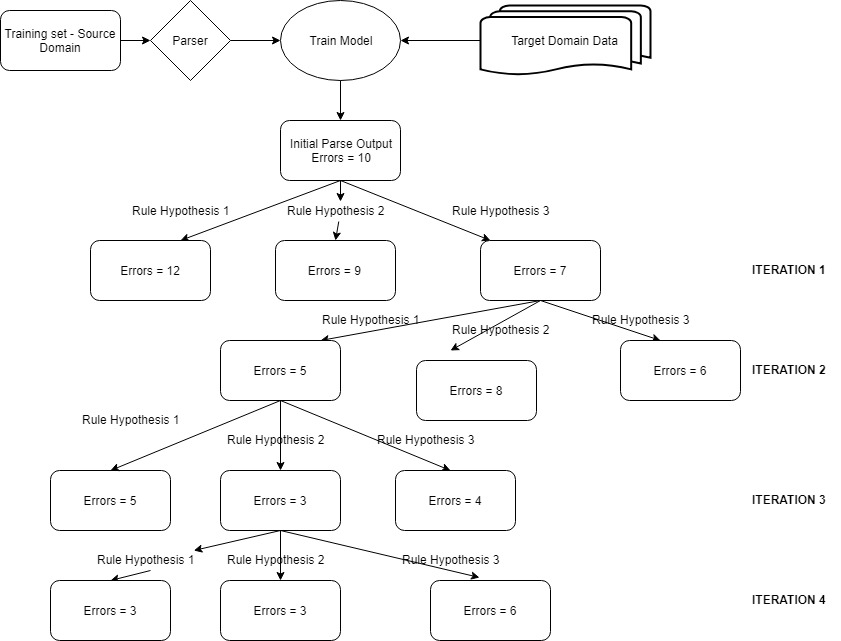
\includegraphics[scale = 0.34]{tbedl.png}
    \centering
    \caption{Reducing dependency label errors via transformation-based error-driven learning\textcolor{white}{try this}}
    \label{fig:tbedl}
\end{figure*}

\textcolor{white}{try this}

\begin{algorithm}[!t]
 \caption{TBL for Domain Adaptation}\label{alg:tbl}
\begin{algorithmic}[1]
\Procedure{$TBL\_learn$}{$training\_data$}
\State $work\_copy\ =\ extract\ text\ from\ training\_data;\ parse\ using\ WSJ\ model$
\State $learned\_rules \gets []$
\Repeat
\LineComment{Generate rule hypothesis from errors in corpus given rule templates}
\State $rule\_hypotheses = generate\_hypotheses(training\_data,work\_copy)$ 
%\vspace{.2em}
\LineComment{calculate improvement score for each rule:  \# errors fixed}
\State $rule\_scores = determine\_scores(rule\_hypotheses, work\_copy)$ 
%\vspace{.1em}
\LineComment{Rank rules given scores; select rule with highest score}
\State $best\_rule, best\_score = argmax(rank\_rules(rule\_hypotheses, rule\_scores)$
%\vspace{.2em}

\LineComment{If best rule causes improvement, apply rule to work copy}
\If{$best\_score > 0$}
\State $work\_copy = apply\_rule(work\_copy, best\_rule)$
\State $learned\_rules \mathrel{+}= best\_rule$
\EndIf
%\LineComment{In the next iteration, we use this changed training data and repeat the process until the number of errors are not reduced anymore.}
\vspace{-1em}
\State \Until{$best\_score <= 0$}
\State \textbf{return} $learned\_rules$
\EndProcedure
\vspace{1em}
\Procedure{$TBL\_apply$}{$learned\_rules, test$}

\State $test\_annotated\ =\  parse\ test\ data\ using\ WSJ\ model$
\LineComment{Apply learned rules in order to test set}
\For{each rule in learned\_rules}
\State $test\_annotated = apply\_rule(test\_annotated, rule)$

\EndFor
\EndProcedure


\end{algorithmic}

\end{algorithm}


We outline the process in algorithm~\ref{alg:tbl}. The learning iterates until there are no more rule hypotheses that would cause a further reduction in errors. During each iteration, based on the templates, the algorithm creates rule hypotheses from the errors found by comparing the working copy to the gold standard. It then chooses the best rule hypothesis that maximally reduces the errors in the working copy and applies this rule to the working copy. %We measure the improvement for each of the rule hypothesis and return the hypothesis (1 or multiple) with most improvement in terms of errors. 
Since the templates that we use are independent of each other, we currently apply the top 10 rules per iteration. Choosing to apply multiple rules speeds up the overall process. To prevent over-generation, we favor the more specific hypothesis if there is a tie in the scores. We then store these rules in the final list of learned rules. %However, our process is flexible enough, such that, this threshold could be changed to any integer.
After the application of the rules chosen in each iteration, we use the updated work copy in the next iteration. %The process finishes when there is no more change in the number of errors. 

After learning, a new text is processed by first having it parsed by the source domain dependency parser and then applying the learned rules in order.

% We instantiate these rule templates on the gold standard corpus and obtain a set of possible rule hypotheses. We do the following iteratively:
% \begin{enumerate}
%     \item We apply the rule hypotheses on the initial state corpus.
%     \item We calculate the reduction in error for each of these rule hypotheses.
%     \item We keep track of the rule hypotheses with the highest improvement in terms of reduction of errors at each iteration. We calculate improvement score($S_i$) as:
%     $$S_i = e_{prev} - e_{curr}$$
%     where $e_{prev}$ is the error prior to applying the rule hypothesis and $e_{curr}$ is the number of errors after applying the rule hypothesis.
%     Since, we do not use dependency labels as variables for our templates, instead of applying the one rule per iteration, we can apply more. For this paper, we choose a threshold of 10. 
%     \item We add these rules with the highest improvement scores to the list of final learned rules.
%     \item We continue until we get no further reduction in errors.
% \end{enumerate}

%After, we get the final list of learned rules from this process, the next step is to apply these rules to the test set. %We evaluate the system by measuring the Labeled Attachment Score (LAS-1) and Labeled Accuracy Scores (LAS-2).

\section{Experimental Setting} \label{sec:exptsetup}

%We report experiments using the following two domains: financial news articles  (WSJ)~\cite{Marcus:1994:PTA:1075812.1075835} and dialogues recorded during a collaborative task (CReST)~\cite{eberhard2010indiana}.  WSJ serves as our source domain, thus we create a parsing model using MATE parser~\cite{bohnet:2010:PAPERS,bohnet2010very}. We parse sentences from CReST using this model. Since the source domain (WSJ) and the target domain (CReST) have differences in dependency label annotation, this introduces some errors in the resulting parse. 

\subsection{Data Sets}
In our current work, we focus on two domains: financial news articles and dialogues in a collaborative task.
We use the Wall Street Journal \cite{Marcus:1994:PTA:1075812.1075835} and the CReST corpus~\cite{eberhard2010indiana} as representative corpora for these two domains. %Wall Street Journal consists of financial articles, news, etc. CReST corpus, on the other hand, comprises of dialogues recorded during a collaborative task.%natural language dialogues between two people, who carry out a certain task with the help of each other. 
%%SK check numbers? - x

These corpora are very dissimilar in nature. On  average, the length of the sentences for WSJ is 24 and 7 for CReST. In terms of linguistic factors, CReST has a subset of WSJ's dependency labels with 10 new labels added.%and 
%%SK why do we care about POS tags? should that be dep labels? - atr: because I was thinking this might also show how different the corpora are, but its not needed.
%has 14 different part of speech tags than WSJ. 
Example sentences from each corpora are shown in table~\ref{tab:samplesentences}. We use WSJ as the source domain and CReST as the target domain.  %We create a parsing model using the MATE parser~\cite{bohnet:2010:PAPERS,bohnet2010very}. We then parse sentences from CReST using this model. %Since the source domain (WSJ) and the target domain (CReST) have differences in dependency label annotation, this introduces some errors in the resulting parse. 

\begin{table}[!t]
\centering
\begin{tabular}{l|l}
\hline
WSJ   & \begin{tabular}[c]{@{}l@{}}
In an Oct. 19 review of " The Misanthrope " at Chicago 's Goodman Theatre \\ ( " Revitalized Classics Take the Stage in Windy City , " Leisure \& Arts ) , \\ the role of Celimene , played by Kim Cattrall , was mistakenly attributed \\ to Christina Haag .\end{tabular} \\ \hline
CReST & \begin{tabular}[c]{@{}l@{}}
it's like as soon - like if I were to close the door it's right next to like the \\ bottom of the floor like where the door closes 
\end{tabular} \\ \hline
%so I went through some - I went through the second room right? \\ \hline    
%can I tell you where that is?   
\end{tabular}
\caption{Sample sentences from Wall Street Journal (WSJ) \& CReST corpus}
\label{tab:samplesentences}
\end{table}



\paragraph{Target Domain}
The CReST corpus consists of 23 dialogues that were manually annotated for dependencies. We randomly select 19 dialogues as our training data and the rest as test. 
since the system needs to learn rule hypotheses from  incorrect predictions of the source domain parser, 
we can safely ignore sentences that were parser completely correctly. For the test data, we use all the sentences from the designated dialogues (with correct and incorrect dependency label predictions). 
%As a part the training part of Transformation Based Error Driven Learning (TBL), the system needs to learn rule hypotheses from the incorrect dependency label prediction, we work on the sentences which show errors in dependency labels. 
Table~\ref{tab:sentdiv} shows the division of sentences for training and test.

\begin{table}[t]
\centering
\begin{tabular}{l|l|c|c}
& \multirow{2}{*}{\# Dialogues} & \multicolumn{2}{c}{\# Sentences} \\ \cline{3-4}
 &  & \multicolumn{1}{l|}{with errors} & \multicolumn{1}{l}{without errors} \\ \hline
Training Set & \multicolumn{1}{|c|}{19} & 4384 & 459 \\
Test Set & \multicolumn{1}{|c|}{4} & 831 & 85 \\ \hline
\end{tabular}
\caption{Target domain training and test set for TBL}
\label{tab:sentdiv}
\end{table}

% \begin{enumerate}[label=Setting \arabic*,leftmargin=*]
% %\setlength\itemsep{2pt}
%     \item We consider all the sentences set aside as the test set has incorrect dependency labels.
%     \item Test set contains a mix of sentences with correct and incorrect dependency labels. 
% \end{enumerate}

\subsection{TBL Components}

\paragraph{Initial State System}
We use the MATE parser~\cite{bohnet:2010:PAPERS} as the initial state annotator. We use 17~181 sentences from WSJ to train the MATE parser. We use this model to parse the sentences from the CReST training set to obtain the initial state annotated text.

\paragraph{Baseline}

We benchmark our results against the performance of the MATE parser trained on WSJ sentences, i.e., the out-of-domain parser, without any modification. We also report results for an in-domain setting where the MATE parser is trained on the CReST training set.


\subsection{Evaluation}
For evaluation, we use the CoNLL-X script. We report the Labeled Attachment Scores  (LAS) and Label Accuracy  (LA) as the primary metrics for evaluating our system. LAS measures the percentage of words which have the correct head and dependency label. LA measures the number of correctly assigned labels. Reporting LA is important  since this measure focuses solely on the accuracy of the labels while LAS also evaluates structural issues in the parse, which we do not address currently. We
also report the exact syntactic match (EM), which measures the percentage of sentences that have correct overall predicted dependency trees.

\section{Experimental Results} \label{expt_results}

In this section, we discuss the outcome of our experiments for the TBL process. The results of applying the rules learned from TBL are given in table~\ref{tab:overall}.
%4 rule templates
%improv>1 -> deprel = 471
%   Labeled   attachment score: 4079 / 5823 * 100 = 70.05 %
%   Unlabeled attachment score: 4308 / 5823 * 100 = 73.98 %
%   Label accuracy score:       5352 / 5823 * 100 = 91.91 %
%2 rule templates
%improv>1 -> deprel = 660
%  SYNTACTIC SCORES:
%   Labeled   attachment score: 4053 / 5823 * 100 = 69.60 %
%   Unlabeled attachment score: 4308 / 5823 * 100 = 73.98 %
%   Label accuracy score:       5163 / 5823 * 100 = 88.67 %
%   Exact syntactic match:      438 / 916 * 100 = 47.82 %
%%SK what does 'WSJ-modeled output' mean? baseline? -x


\begin{table}[t]
\centering
%\resizebox{\textwidth}{!}{%   
\begin{tabular}{l|l|r|rrr|}
 & \multicolumn{1}{c|}{Setting} & \# Incorrect  & LAS & LA & EM \\ \hline
1 & Baseline (trained on WSJ) & 2~112 & 59.02  & 63.73 & 8.41  \\
%2 & In-domain baseline (trained on CReST)& 1~289 & \textbf{72.57}  & 77.86 & \textbf{53.49}   \\
2 & In-domain baseline (trained on CReST)& 572 & \textbf{87.39}  & 90.18 & \textbf{67.58}   \\
3 & Rule Templates (1+2) & 600 & 69.91  & 89.70 & 48.03 \\
4 & Rule Templates (1+2+3+4) & {451} &{\textbf{\textit{70.10}}} &
{\textbf{92.25}} & {\textbf{\textit{48.80}}}  \\
%1 & Baseline (WSJ-parsed output) & 2~112 & 59.02  & 63.73 & 8.41  \\
\hline
\end{tabular}%
%}
\caption{Results of applying TBL rules on test set.}
\label{tab:overall}
\end{table}


The first setting is our baseline. We evaluate the performance of our system against the results of parsing the sentences from the test set with the model trained on WSJ. The second baseline consists of an in-domain parser trained on the small CReST training set. Settings 3 and 4 evaluate the performance of the learned rules. The third setting derives rule hypotheses instantiated by 2 rule templates (rule templates 1 \& 2). Since rule templates 1 \& 2 are more specific (it accounts for lemma as well as part of speech tags), we add more general templates such as POS tags specifically (rule templates 3 \& 4) to investigate if that leads to a significant difference in the results. %We also report the in-domain results as setting 4.%Thus, this setting evaluates the results of applying rules learned from 4 rule templates (rule templates 1, 2, 3 and 4). We include the results of in-domain parsing as setting 4.
%%SK OK, can we also mention what the 2 and 4 templates are? Did you adjust the numbers in the table after you sorted the templates in sec. 4.2? And can you tell us why these two settings? - x

From table~\ref{tab:overall}, we observe that applying TBL has a significant effect on the quality of the predicted dependency labels, with an improvement in LAS of almost 20\% absolute over the out-of-domain parses. The number of completely correct sentences shows an improvement of 40\% absolute over this baseline. We also see that extending the set of templates to include less-specific templates (templates 3 and 4) using POS tags information, has a minimal effect on LAS but increases label accuracy (LA) by 2.5\% absolute. 

\begin{table}[t]
\centering
\begin{tabular}{l|r|rrr|}
\multicolumn{1}{c|}{\multirow{2}{*}{Label}} & \multirow{2}{*}{\# in Gold} & \multicolumn{3}{c|}{\% Correct} \\ \cline{3-5}
\multicolumn{1}{c|}{} &  & baseline &2 templates & 4 templates \\ \hline
INTJ & 690 & 0 & 98.26 & 99.71 \\
ROOT* & 195 & 0 & 63.59 & 77.44 \\ \hline
%VMOD & 1 & 0 & 0 & 0 \\ \hline
\end{tabular}
\caption{Accuracy in predicting CReST-specific labels.}
\label{tab:labelcomp}
\end{table}



%When comparing the TBL results  to the in-domain baseline, we notice that the baseline reaches an LAS that is about 2.5\% higher than the TBL results, but the TBL approach reaches considerably higher results with regard to LA (92.25\% vs.\ 77.86\%). The different trends can be explained by the fact that we are currently restricting the TBL approach to functional changes, and we ignore structural errors. Since the LAS evaluates both aspects, we see that the in-domain parser fares better in this respect. However, the LA, which only evaluates dependency labels, shows that our method is very successful in improving the labels. 

When comparing the TBL results  to the in-domain baseline, we notice that the baseline reaches an LAS considerably higher than the TBL results, but the TBL approach using all 4 templates reaches higher results with regard to LA (around 2\% improvement). The different trends can be explained by the fact that we are currently restricting the TBL approach to functional changes, and we ignore structural errors. Since LAS evaluates both aspects, we see that the in-domain parser fares better in this respect. However, the LA, which only evaluates dependency labels, shows that our method is successful in improving the labels. Since the results of the experiment with 2 templates are similar to the in-domain treebank, we assume that we need to experiment with more specific templates in the future.


%Since we do not revise dependency heads, the unlabeled attachment score remains the same at 73.98\% for settings 1,2 \&3 but increases to 77.13\% for setting 4. This leads to a higher LAS than the TBL setting. However, LA is significantly higher for the TBL setting  with more than 14\% improvement which shows the effectiveness of applying TBL to reduce the number of incorrect dependency labels. The results will be comparable when we add structural transformations (i.e., correcting dependency heads) in our TBL settings.
%Although LAS is higher in in-domain setting - owing to the improved UAS - than setting 3, LA is significantly higher for the TBL setting. (14.39\% improvement; with more than 50\% improvement in reducing label confusions). 
%%SK please add -x 

There are 10 dependency labels in CReST which do not occur in WSJ. Out of these, 2 labels  (ROOT\textsc{*}, INTJ) occur in the test data. ROOT\textsc{*} is used for words whose head is missing because the sentence was interrupted; and INTJ is used for interjections. Since WSJ does not use these labels, these are predicted incorrectly in all the cases in the out-of-domain baseline. 

We investigate the number of times these labels have been corrected by TBL. Table~\ref{tab:labelcomp} shows the results. As expected, the labels do not show up in the baseline setting. For the settings using 2 or 4 templates, there is a significant improvement for the labels INTJ and ROOT\textsc{*}. 
%%SK I think that is an annotation error? - x
% However, the label VMOD has not been predicted accurately (predicted as ADV). We examine the training set for contextual information on the label. % atr - I don't know how to write this
% For the same context (parent/dependents/lemma), the label ADV appears 54 times whereas the label VMOD appears once. 


\begin{table}[t]
\resizebox{\textwidth}{!}{%

\begin{tabular}{ccccccccc} 
\hline
Rule Template & Lemma (self) & Pos (self) & Lemma (head) & POS (head) & Lemma (children) & POS (children) & Deprel & Improvement \\ \hline
RT2 & okay & UH & (root word) & (root word) & - & - & INTJ & 1292 \\
RT2 & um & UH & (root word) & (root word) & - & - & INTJ & 386 \\
RT2 & be & VBZ & (root word) & (root word) & - & - & ROOT & 384 \\
RT2 & alright & UH & (root word) & (root word) & - & - & INTJ & 216 \\
RT2 & yeah & UH & (root word) & (root word) & - & - & INTJ & 205 \\
RT2 & the & DT & (root word) & (root word) & - & - & ROOT* & 131 \\
RT3 & and & CC & be & VBZ & (no children) & (no children) & COORD & 117 \\
RT2 & go & VBI & (root word) & (root word) & - & - & ROOT & 100 \\
RT3 & that & DDT & be & VBZ & (no children) & (no children) & SBJ & 83 \\
RT2 & well & UH & (root word) & (root word) & - & - & INTJ & 77 \\ \hline
\end{tabular}%
}
\caption{Top learned rules for the setting using 2 templates.}
\label{tab:2templatestoprules}
\end{table}

Table~\ref{tab:2templatestoprules} and \ref{tab:4templatestoprules} show  the 10 learned rules with the highest scores, for the setting with 2 or 4 templates respectively. We can observe that many of the rules concern the labels INTJ and ROOT\textsc{*}. Since these labels do not appear in the source domain, applying rule hypotheses specific to these labels leads to the highest gains. 

To have a closer look, we extracted the most frequent label confusions for each setting after parsing and TBL domain adaptation. The results are shown in table~\ref{tab:depconf}. For the baseline, the most frequently incorrect label is INTJ, followed by ROOT and ROOT\textsc{*}. By applying TBL, we have countered the most frequent label confusion as evident from the settings using 2 or 4 templates, where the numbers are lower across the board, but also the types of confusion are more typical of standard parsing issues (e.g., subject (SBJ) vs.\ predicate (PRD)).


\begin{table}[t]
\centering
\resizebox{\textwidth}{!}{%
\begin{tabular}{ccccccccc}
\\ \hline
Rule Template & Lemma (self) & POS (self) & Lemma (head) & POS (head) & Lemma (children) & POS (children) & Deprel & Improvement \\ \hline
RT4 & - & UH & - & (root word) & - & - & INTJ & 2886 \\
RT5 & - & UH & - & (root word) & - & (no children) & INTJ & 2766 \\
RT2 & okay & UH & (root word) & (root word) & - & - & INTJ & 1292 \\
RT3 & okay & UH & (root word) & (root word) & (no children) & (no children) & INTJ & 1271 \\
RT4 & - & AP & - & (root word) & - & - & INTJ & 453 \\
RT5 & - & AP & - & (root word) & - & (no children) & INTJ & 438 \\
RT2 & um & UH & (root word) & (root word) & - & - & INTJ & 386 \\
RT2 & be & VBZ & (root word) & (root word) & - & - & ROOT & 384 \\
RT3 & um & UH & (root word) & (root word) & (no children) & (no children) & INTJ & 383 \\
RT5 &  & XY &  & (root word) &  & (no children) & ROOT* & 268 \\ \hline
\end{tabular}%
}
\caption{Top learned rules for the setting using 4 templates.}
\label{tab:4templatestoprules}
\end{table}



% \begin{table}[!htb]
% \centering
% \begin{tabular}{c|c|c|c}
% \multicolumn{2}{c|}{Setting - 2} & \multicolumn{2}{c}{Setting - 3} \\ \hline
% Best Rule Template & Improvement & Best Rule Template & Improvement \\ \hline
% RT2 & 1292 & RT4 & 2886 \\
% RT2 & 386 & RT5 & 2766 \\
% RT2 & 384 & RT2 & 1292 \\
% RT2 & 216 & RT3 & 1271 \\
% RT2 & 205 & RT4 & 453 \\
% RT2 & 131 & RT5 & 438 \\
% RT3 & 117 & RT2 & 386 \\
% RT2 & 100 & RT2 & 384 \\
% RT3 & 83 & RT3 & 383 \\
% RT2 & 77 & RT5 & 268 \\ \hline
% \end{tabular}
% \caption{Top 10 rules learned by the system}
% \label{tab:bestrules}
% \end{table}


% \begin{table}[]
% \centering
% \resizebox{\textwidth}{!}{%
% \begin{tabular}{llcccccccccccccccc}
%  &  & \multicolumn{7}{c}{Setting - 2} & \multicolumn{9}{c}{Setting - 3} \\
% Rule Template & Lemma (self) & Pos-self & Lemma (head) & POS (head) & Lemma (children) & POS (children) & Deprel & Improvement & Rule Template & Lemma (self) & POS (self) & Lemma (head) & POS (head) & Lemma (children) & POS (children) & Deprel & Improvement \\
% RT2 & okay & UH & (root word) & (root word) & - & - & INTJ & 1292 & RT4 & - & UH & - & (root word) & - & - & INTJ & 2886 \\
% RT2 & um & UH & (root word) & (root word) & - & - & INTJ & 386 & RT5 & - & UH & - & (root word) & - & (no children) & INTJ & 2766 \\
% RT2 & be & VBZ & (root word) & (root word) & - & - & ROOT & 384 & RT2 & okay & UH & (root word) & (root word) & - & - & INTJ & 1292 \\
% RT2 & alright & UH & (root word) & (root word) & - & - & INTJ & 216 & RT3 & okay & UH & (root word) & (root word) & (no children) & (no children) & INTJ & 1271 \\
% RT2 & yeah & UH & (root word) & (root word) & - & - & INTJ & 205 & RT4 & - & AP & - & (root word) & - & - & INTJ & 453 \\
% RT2 & the & DT & (root word) & (root word) & - & - & ROOT* & 131 & RT5 & - & AP & - & (root word) & - & (no children) & INTJ & 438 \\
% RT3 & and & CC & be & VBZ & (no children) & (no children) & COORD & 117 & RT2 & um & UH & (root word) & (root word) & - & - & INTJ & 386 \\
% RT2 & go & VBI & (root word) & (root word) & - & - & ROOT & 100 & RT2 & be & VBZ & (root word) & (root word) & - & - & ROOT & 384 \\
% RT3 & that & DDT & be & VBZ & (no children) & (no children) & SBJ & 83 & RT3 & um & UH & (root word) & (root word) & (no children) & (no children) & INTJ & 383 \\
% RT2 & well & UH & (root word) & (root word) & - & - & INTJ & 77 & RT5 &  & XY &  & (root word) &  & (no children) & ROOT* & 268
% \end{tabular}%
% }
% \end{table}


% \begin{table}[!t]
% \centering
% \resizebox{\textwidth}{!}{%
% \begin{tabular}{ccc|ccc|ccc|ccc}
% \multicolumn{3}{c|}{Setting 1} & \multicolumn{3}{c|}{Setting 2} & \multicolumn{3}{c|}{Setting 3} & \multicolumn{3}{c}{Setting 4} \\ \hline
% Gold & Predicted & Counts & Gold & Predicted & Counts & Gold & Predicted & Counts & \multicolumn{1}{c}{Gold} & \multicolumn{1}{c}{Predicted} & \multicolumn{1}{c}{Counts} \\ \hline
% INTJ & ROOT & 354 & ROOT* & ROOT & 39 & ROOT* & ROOT & 38 & 57 & ROOT & NMOD \\
% INTJ & DEP & 210 & SBJ & PRD & 20 & SBJ & PRD & 25 & 47 & LOC & ROOT \\
% ROOT & NMOD & 136 & ROOT* & NMOD & 20 & ROOT & ROOT* & 21 & 36 & NMOD & ROOT \\
% ROOT* & NMOD & 100 & LOC & NMOD & 19 & DIR & LOC & 19 & 33 & ROOT* & NMOD \\
% INTJ & NMOD & 85 & ROOT & ROOT* & 17 & DIR & ADV & 17 & 27 & LOC & DIR \\
% LOC & NMOD & 55 & DIR & ADV & 15 & LOC & NMOD & 15 & 25 & ROOT* & ROOT \\
% COORD & DEP & 38 & ROOT & NMOD & 13 & TMP & ADV & 10 & 23 & VC & NMOD \\
% ROOT & COORD & 37 & DIR & NMOD & 12 & LOC & ADV & 10 & 22 & SBJ & NMOD \\
% LOC & LOC-PRD & 35 & LOC & ADV & 11 & ROOT & NMOD & 8 & 21 & P & NMOD \\
% LOC & PRD & 33 & PMOD & NMOD & 10 & OBJ & SBJ & 8 & 20 & NMOD & PRD \\ \hline
% \end{tabular}%
% }
% \caption{The 10 most frequent label confusions across the different settings.}
% \label{tab:depconf}
% \end{table}


\begin{table}[!t]
\centering
\resizebox{\textwidth}{!}{%
\begin{tabular}{ccc|ccc|ccc}
\multicolumn{3}{c|}{Baseline} & \multicolumn{3}{c|}{2 Templates} & \multicolumn{3}{c}{4 Templates} \\ \hline
Gold & Predicted & Counts & Gold & Predicted & Counts & Gold & Predicted & Counts \\ \hline
INTJ & ROOT & 354 & ROOT* & ROOT & 39 & ROOT* & ROOT & 38 \\
INTJ & DEP & 210 & SBJ & PRD & 20 & SBJ & PRD & 25 \\
ROOT & NMOD & 136 & ROOT* & NMOD & 20 & ROOT & ROOT* & 21 \\
ROOT* & NMOD & 100 & LOC & NMOD & 19 & DIR & LOC & 19 \\
INTJ & NMOD & 85 & ROOT & ROOT* & 17 & DIR & ADV & 17 \\
LOC & NMOD & 55 & DIR & ADV & 15 & LOC & NMOD & 15 \\
COORD & DEP & 38 & ROOT & NMOD & 13 & TMP & ADV & 10 \\
ROOT & COORD & 37 & DIR & NMOD & 12 & LOC & ADV & 10 \\
LOC & LOC-PRD & 35 & LOC & ADV & 11 & ROOT & NMOD & 8 \\
LOC & PRD & 33 & PMOD & NMOD & 10 & OBJ & SBJ & 8 \\ \hline
\end{tabular}%
}
\caption{The 10 most frequent label confusions across the different settings.}
\label{tab:depconf}
\end{table}


%\clearpage
\section{Discussion} \label{conclusion}
% x

In this paper, we introduce transformation-based error-driven learning (TBL) for domain adaptation in dependency parsing. Since there tend to be significant differences between annotation schemes of different corpora from different domains, we focus on methods that can address those differences systematically along with differences due to the domain itself.  When a text is parsed with a model trained on one domain, it leads to a significant number of incorrect predictions, especially for dependency labels. %This is because source and target might have different labels. As we show in our analysis, this is indeed the case. 
We address this problem in our work by using TBL to learn rules from a small target domain training set and a small set of manually defined rule templates. % by iteratively applying rule hypotheses and learning the rules with the best improvement. 
In comparison to a pure out-of-domain parser, we observe a significant increase in the labeled attachment scores (\char`\~20\%), labeled accuracy (\char`\~30\%) and exact match (\char`\~40\%) for WSJ as source and CReST as target corpus. The observed improvement is largely due to the labels that are used in CReST, but do not occur in WSJ since those are mislabeled consistently by the out-of-domain parser. However, when we apply TBL, these labels are corrected in most of the cases. When we compare our results to an in-domain parser, the results show that the TBL approach is very
 good at correcting the dependency labels, but we need to extend the approach and use more specific templates and cover structural errors as well to be able to compete with the in-domain parser with regard to LAS. 

Our method is flexible in that any number of variables can be used in the templates, and it can be extended to cover structural changes, i.e., to correct dependency head annotations. In addition, the templates are valid across different target domains.

As a part of our future work, we plan to evaluate the effectiveness of this method for multiple domains. We will also introduce new variables in our rule templates including contextual information on dependency labels. In addition to correcting dependency labels, we will extend the method to correct predicted dependency heads by introducing new templates. This will need to be accompanied by a check to ensure that the resulting analysis is still a valid dependency graph. 


%%%%%%%%%%%%%%%%
% Chapter 8 - Conclusion
%%%%%%%%%%%%%%%%

\chapter{Conclusion}
%%%%%%%%%%%%%%%%
% Appendices
%%%%%%%%%%%%%%%%

\begin{appendices}

%Some Table of Contents entry formatting
\addtocontents{toc}{\protect\renewcommand{\protect\cftchappresnum}{\appendixname\space}}
\addtocontents{toc}{\protect\renewcommand{\protect\cftchapnumwidth}{6em}}

%Begin individual appendices, separated as chapters

\chapter{Placeholder}
Lorem ipsum dolor sit amet, consectetur adipiscing elit, sed do eiusmod tempor incididunt ut labore et dolore magna aliqua. Ut enim ad minim veniam, quis nostrud exercitation ullamco laboris nisi ut aliquip ex ea commodo consequat. Duis aute irure dolor in reprehenderit in voluptate velit esse cillum dolore eu fugiat nulla pariatur. Excepteur sint occaecat cupidatat non proident, sunt in culpa qui officia deserunt mollit anim id est laborum.

\chapter{Placeholder}
Lorem ipsum dolor sit amet, consectetur adipiscing elit, sed do eiusmod tempor incididunt ut labore et dolore magna aliqua. Ut enim ad minim veniam, quis nostrud exercitation ullamco laboris nisi ut aliquip ex ea commodo consequat. Duis aute irure dolor in reprehenderit in voluptate velit esse cillum dolore eu fugiat nulla pariatur. Excepteur sint occaecat cupidatat non proident, sunt in culpa qui officia deserunt mollit anim id est laborum.

\end{appendices}

%%%%%%%%%%%%%%%%
% References
%%%%%%%%%%%%%%%%
%\begin{singlespace}  % use single-line spacing for multi-line text within a single reference
%	\setlength\bibitemsep{\baselineskip}  %manually set separataion betwen items in bibliography to double space
%	\printbibliography[heading=bibintoc,title={References}]
%\end{singlespace}

%\printbibliography[heading=bibintoc,title={References}]
%\addcontentsline{toc}{chapter}{References}  %add References section to Table of Contents

%%%%%%%%%%%%%%%%
% Vita 
% Only for PhD students
% Masters students remove this line
%%%%%%%%%%%%%%%%
%\chapter*{Vita}
\addtocontents{toc}{
 \unexpanded{\unexpanded{\renewcommand{\cftchapdotsep}{\cftnodots}}}%  
}
\addcontentsline{toc}{chapter}{Curriculum Vitae}

\doublespacing
Vita may be provided by doctoral students only. The length of the vita is preferably one page. It may include the place of birth and should be written in third person. This vita is similar to the author biography found on book jackets.

\pagenumbering{gobble}

\bibliographystyle{plainnat}
\bibliography{references}

\end{document}
